

%%%%%%%%%%%%%%%%%%%%%%%%%%%%%%%%%%%%%%%%%%%%%%%%%%%%%%%%%%%%%%%%%%%%%%%%%%%%%
%                                                                           %
%          LaTeX File for Doctor (Master) Thesis of ECNU                    %
%            华东师范大学博士(硕士)论文模板 ____lizb                      %
%                                                                           %
%%%%%%%%%%%%%%%%%%%%%%%%%%%%%%%%%%%%%%%%%%%%%%%%%%%%%%%%%%%%%%%%%%%%%%%%%%%%%


\documentclass[12pt,openany,a4paper,fancyhdr,oneside]{ctexbook}

%draft 选项可以使插入的图形只显示外框,以加快预览速度。
%\documentclass[11pt,a4paper,openany,draft]{book}

\usepackage[CJKbookmarks]{hyperref}
\usepackage{shortvrb,indentfirst,ulem,makeidx}
\usepackage{fancyhdr}
\usepackage{graphicx}
\usepackage{indentfirst,latexsym,amsthm,colortbl,subfigure,clrscode}
\usepackage{algorithm}
\usepackage[noend]{algorithmic}
%\usepackage[ruled, vlined, linesnumbered]{algorithm2e}
\usepackage{bm}                     % 处理数学公式中的黑斜体的宏包
\usepackage{amsmath}                % AMSLaTeX宏包 用来排出更加漂亮的公式
\usepackage{amssymb}                % AMSLaTeX宏包 用来排出更加漂亮的公式
\usepackage{mathrsfs}
\usepackage[subnum]{cases}
\usepackage[numbers,sort&compress]{natbib} 
\usepackage{hypernat}
\usepackage{geometry}
\usepackage{multirow}
\usepackage{times}
\usepackage{fontspec}
\usepackage{libertine}
\usepackage{url}
\usepackage{caption}
\usepackage{titletoc}
\usepackage{slashbox}
\usepackage{array}
\usepackage{indentfirst} 
\usepackage{color}
\usepackage{epstopdf}
\usepackage{rotating}
\usepackage{supertabular} %supertabular表格宏包
\usepackage{colortbl} %彩色表格宏包
\usepackage{booktabs} %表格线宏包
\usepackage{longtable} 
\usepackage{bigstrut,multirow,rotating}

%设置bib的行间距
\usepackage{setspace}
%设置章节第一页的顶边距
%\usepackage{titlesec}
%\usepackage{etoolbox}
\makeindex
\pagestyle{fancy}
\newcommand{\comment}[1]{}
\renewcommand{\headrulewidth}{0.4pt}
\fancyfoot[CO,CE]{\thepage}

\renewcommand{\algorithmicrequire}{\textbf{输入:}}
\renewcommand{\algorithmicensure}{\textbf{输出:}}
\newcommand{\loflabel}{图}%在图目录编号前添加Tab.
\newcommand{\lotlabel}{表}

\newcommand{\ie}{\textit{i.e., }}
\newcommand{\aka}{\textit{i.e., }}
\newcommand{\eg}{\textit{e.g., }}
\newcommand{\etal}{\textit{et al. }}


%                    根据自己正文需要做的一些定义                 %
%==================================================================
\def\diag{{\rm diag}}
\def\rank{{\rm rank}}
\def\RR{{\cal R}}
\def\NN{{\cal N}}
\def\R{{\mathbb R}}
\def\C{{\mathbb C}}
\let\dis=\displaystyle

\def\p{\partial}
\def\f{\frac}
\def\mr{\mathrm}
\def\mb{\mathbf}
\def\mc{\mathcal}
\def\b{\begin}
\def\e{\end}

\newtheorem{thm1}{Theorem}[part]
\newtheorem{thm2}{Theorem}[section]
\newtheorem{thm3}{Theorem}[subsection]
\newtheorem{them}[thm2]{定理}
\newtheorem{theorem}[thm2]{定理}
\newtheorem{defn}[thm2]{定义}
\newtheorem{define}[thm2]{定义}
\newtheorem{ex}[thm2]{例}
\newtheorem{exs}[thm2]{例}
\newtheorem{example}[thm2]{例}
\newtheorem{prop}[thm2]{命题}
\newtheorem{lemma}[thm2]{引理}
\newtheorem{cor}[thm2]{推论}
\newtheorem{remark}[thm2]{注释}
\newtheorem{notation}[thm2]{记号}
\newtheorem{abbre}[thm2]{缩写}
%\newtheorem{algorithm}[thm2]{算法}
\newtheorem{problem}[thm2]{问题}
%重新设置证明的其实标题
\floatname{algorithm}{算法}
\renewcommand{\proofname}{\textit{证明}}
\usepackage{etoolbox}  % patch def of algorithmic environment
\makeatletter
\patchcmd{\algorithmic}{\addtolength{\ALC@tlm}{\leftmargin} }{\addtolength{\ALC@tlm}{\leftmargin}}{}{}
\makeatother
\renewcommand\algorithmiccomment[1]{%
	\hfill\#\ #1%
}

\newcommand{\yihao}{\fontsize{26pt}{36pt}\selectfont}           % 一号, 1.4 倍行距
\newcommand{\erhao}{\fontsize{22pt}{28pt}\selectfont}          % 二号, 1.25倍行距
\newcommand{\xiaoer}{\fontsize{18pt}{18pt}\selectfont}          % 小二, 单倍行距
\newcommand{\sanhao}{\fontsize{16pt}{24pt}\selectfont}        % 三号, 1.5倍行距
\newcommand{\xiaosan}{\fontsize{15pt}{22pt}\selectfont}        % 小三, 1.5倍行距
\newcommand{\sihao}{\fontsize{14pt}{21pt}\selectfont}            % 四号, 1.5 倍行距
\newcommand{\banxiaosi}{\fontsize{13pt}{19.5pt}\selectfont}    % 半小四, 1.5倍行距
\newcommand{\xiaosi}{\fontsize{12pt}{18pt}\selectfont}            % 小四, 1.5倍行距
%\newcommand{\xiaosi}{\fontsize{12pt}{12pt}\selectfont}            % 小四, 1倍行距
\newcommand{\dawuhao}{\fontsize{11pt}{11pt}\selectfont}       % 大五号, 单倍行距
\newcommand{\wuhao}{\fontsize{10.5pt}{15.75pt}\selectfont}    % 五号, 单倍行距


%============================ 可以自定义文字块 ================================%

\newcommand{\aaa}{Example}
\newcommand{\bbb}{\aaa \aaa \aaa}
\newcommand{\ccc}{\bbb \bbb \bbb \bbb \bbb

\bbb \bbb \bbb \bbb \bbb }
\newcommand{\abc}{abcdefg1234567890}
\newcommand{\upabc}{ABCDEFGHIJK}


%%% ----------------------------------------------------------------------

%设置每章标题前后的间距
\CTEXsetup[beforeskip = 0pt]{chapter}
\CTEXsetup[afterskip = 20pt]{chapter}
\setlength{\baselineskip}{25pt}  %%正文设为25磅行间距

%============================= 版芯控制 ================================%
\setlength{\oddsidemargin}{0.57cm} 
\setlength{\evensidemargin}{\oddsidemargin}
\voffset-6mm \textwidth=150mm \textheight=230mm \headwidth=150mm
%\rightmargin=35mm
%                                                                       %

%============================= 页面设置 ================================%
%-------------------- 定义页眉和页脚 使用fancyhdr 宏包 -----------------%
% 定义页眉与正文间双隔线
\newcommand{\makeheadrule}{%
\makebox[0pt][l]{\rule[.7\baselineskip]{\headwidth}{0.4pt}}%
\rule[0.85\baselineskip]{\headwidth}{0.4pt} \vskip-.8\baselineskip}
\lhead{}
\chead{华东师范大学博士论文}
\rhead{}
\makeatletter

%新加的,为每章首页添加页眉
\makeatletter
\let\ps@plain\ps@fancy
\makeatother

\renewcommand{\headrule}{%
{\if@fancyplain\let\headrulewidth\plainheadrulewidth\fi
\makeheadrule}} \makeatother

\newcommand{\adots}{\mathinner{\mkern 2mu%
\raisebox{0.1em}{.}\mkern 2mu\raisebox{0.4em}{.}%
\mkern2mu\raisebox{0.7em}{.}\mkern 1mu}}

\setmainfont{Times New Roman}
\dottedcontents{chapter}[1.5cm]{\xiaosi\heiti}{3.8em}{9.5pt}
\dottedcontents{section}[1.5cm]{\xiaosi\heiti}{2.8em}{9.5pt}



%=============================== 正文部分 ================================%


\begin{document}
\pagestyle{empty}
\setlength{\baselineskip}{25pt}  %%正文设为25磅行间距
\vspace{-2.0cm}
\noindent{{\zihao{4} {\large 2017} 届博士学位论文}}\\
\vspace{-0.8cm}
\begin{flushleft}
\hspace{-0.5cm}
\renewcommand\arraystretch{1.5}
\begin{tabular}{l}
\noindent{{\zihao{4} 分类号:\underline{\qquad\qquad\qquad}}}  \\ 
\noindent{{\zihao{4} 密~~~~级:\underline{\qquad\qquad\qquad}}}\\ 
\end{tabular}
\hskip 4.1cm
\renewcommand\arraystretch{1.5}
\begin{tabular}{l}
\noindent{{\zihao{4} 学校代码:\underline{~~~~~~10269~~~~~~}}}\\ 
\noindent{{\zihao{4} 学~~~~~~~~号:\underline{~~~~~~~~~~~~~~~~~~~~~~}}}\\ 
\end{tabular}
\end{flushleft}


\vskip 1.8cm

\begin{center}
\hskip 0.5cm
  \scalebox{1.0}{
\includegraphics[width=2.6cm]{fig/ecnu_logo.png}}
  \hspace{0.3cm}
\scalebox{1.0}{
\includegraphics[width=10.5cm]{fig/ecnulabel.png}}
\vskip 0.5cm
{\textbf{{\xiaoer East China Normal University}}}\\ \vskip 0.2cm
{\textbf{\erhao 博~士~学~位~论~文}}\\ \vskip 0.2cm
{\textbf{{\xiaoer DOCTORAL DISSERTATION}}}\\
\end{center}


\vskip 1.0cm

\begin{center}
{\erhao \bf 论文题目:\underline{基于矩阵分解的个性化推荐系统}}
\end{center}

\vskip 1.0cm 
\begin{center}

\renewcommand\arraystretch{1.5}
	\begin{tabular}{l}
{\sihao \bf 院\qquad\ \ \ 系:}\\ 
{\sihao \bf 专~业~名~称:}\\ 
{\sihao \bf 研~究~方~向:}\\ 
{\sihao \bf 指~导~教~师:}\\ 
{\sihao \bf 学位申请人:}
\end{tabular}
\begin{tabular}c
{\sihao \bf  ~~计算机科学与软件工程学院}               \\ 
\hline {\sihao \bf ~~软件工程 }              \\ 
\hline {\sihao \bf ~~推荐系统~~}\\ 
\hline {\sihao \bf ~~ }  \\
\hline{\sihao \bf  ~~ }      \\ 
\hline
\end{tabular}


\end{center}

\vskip 2.0cm
\begin{center}
{\sihao 2017年04月}
\end{center}
%额外空白页
\clearpage
\phantom{s}
\clearpage
\newpage

\pagestyle{empty}

\noindent{\large Dissertation for doctor degree in 2017}
\hskip 1.83cm {\large University Code: 10269}\\
\hspace*{\fill} {\large Student ID: ~~~~~}

\vskip 2cm

\begin{center}
{\Huge $\mathbb{EAST}\,\mathbb{CHINA}\,\mathbb{NORMAL}\,
\mathbb{UNIVERSITY}$}
\end{center}

\vskip 3cm

\begin{center}
\bfseries{\scshape{\huge Personalized Recommender Systems based on  Matrix Factorization}}\\
\end{center}

\vskip 2cm {\large
\begin{center}
\begin{tabular}{l}
Department:\\
\\
Major:\\
Research direction:\\

Supervisor:\\
Candidate:
\end{tabular}
\begin{tabular}c
~~~School of Computer Science and\\
\hline~~~ Software Engineering    \\
\hline ~~~Software Engineering    \\
\hline ~~~Recommender Systems\\ 
\hline ~~~\\
\hline ~~~  \\
\hline
\end{tabular}
\end{center}}

\vskip 30mm

\begin{center}
{\Large 2017.04}
\end{center}
%额外空白页
\clearpage
\phantom{s}
\clearpage
\newpage
\pagestyle{empty}
\centerline{\bf\Large 华东师范大学学位论文原创性声明}

\vskip 1cm

\normalsize \indent
郑重声明:本人呈交的学位论文《基于矩阵分解的个性化推荐系统》,是在华东师范大学攻读硕士/博士(请勾选)学位期间,在导师的指导下进行的研究工作及取得的研究成果。除文中已经注明引用的内容外,本论文不包含其他个人已经发表或撰写过的研究成果。对本文的研究做出重要贡献的个人和集体,均已在文中作了明确说明并表示谢意。
$$\\  $$

\qquad\qquad{作者签名}:$\underline{\qquad\qquad\qquad }$
\qquad \qquad\qquad \mbox {日期}:\qquad 年 \qquad  月 \qquad  日


\vskip 1cm

\centerline{\bf\Large 华东师范大学学位论文著作权使用声明}

\vskip 1cm

《基于矩阵分解的个性化推荐系统》系本人在华东师范大学攻读学位期间在导师指导下完成的硕士/博士(请勾选)学位论文,本论文的研究成果归华东师范大学所有。本人同意华东师范大学根据相关规定保留和使用此学位论文,并向主管部门和相关机构如国家图书馆、中信所和“知网”送交学位论文的印刷版和电子版;允许学位论文进入华东师范大学图书馆及数据库被查阅、借阅;同意学校将学位论文加入全国博士、硕士学位论文共建单位数据库进行检索,将学位论文的标题和摘要汇编出版,采用影印、缩印或者其它方式合理复制学位论文。

本学位论文属于(请勾选)

(  )1.经华东师范大学相关部门审查核定的“内部”或“涉密”学位论文*,
于     年    月    日解密,解密后适用上述授权。

(  )2.不保密,适用上述授权。
$$\\ $$
\qquad\qquad \mbox{导师签名}:$\underline{\qquad\qquad\qquad\qquad}$
\qquad\qquad \mbox {本人签名}:$\underline{\qquad\qquad\qquad\qquad }$

\vskip 0.5cm

$\rightline{ \qquad 年 \qquad  月 \qquad  日 \qquad\qquad}$

%这里改成了0.5,之前是1
\vskip 1cm

* “涉密”学位论文应是已经华东师范大学学位评定委员会办公室或保密委员会审定过的学位论文(需附获批的《华东师范大学研究生申请学位论文“涉密”审批表》方为有效),未经上述部门审定的学位论文均为公开学位论文。此声明栏不填写的,默认为公开学位论文,均适用上述授权)。
%额外空白页
\clearpage
\phantom{s}
\clearpage
\newpage
\pagestyle{empty}
$$\\ \\ \\ $$

\centerline{\bf\Large $\underline{\mbox{\kaishu{~~~~~~~~}}}\,\,
$博士学位论文答辩委员会成员名单}

\vskip 10mm

\begin{center}
{\large
\begin{tabular}{| p{25mm}| p{25mm}| p{45mm}| p{25mm}|}\hline
\vfill\hfill{\heiti 姓名}\hspace*{\fill} &\vfill\hfill{\heiti 职称}\hspace*{\fill} &
\vfill\hfill{\heiti 单位}\hspace*{\fill} &\vfill\hfill {\heiti 备注} \hspace*{\fill} \\[6pt]\hline
\vfill\hfill{}\hspace*{\fill} &\vfill\hfill{}\hspace*{\fill} &\vfill\hfill{}\hspace*{\fill} & \vfill\hfill {\heiti }\hspace*{\fill} \\[6pt]\hline
\vfill\hfill{}\hspace*{\fill} &\vfill\hfill{}\hspace*{\fill} &\vfill\hfill{}\hspace*{\fill} & \vfill\hfill {}\hspace*{\fill} \\[6pt]\hline
\vfill\hfill{}\hspace*{\fill} &\vfill\hfill{}\hspace*{\fill} &\vfill\hfill{}\hspace*{\fill} & \vfill\hfill {}\hspace*{\fill} \\[6pt]\hline
\vfill\hfill{}\hspace*{\fill} &\vfill\hfill{}\hspace*{\fill} &\vfill\hfill{}\hspace*{\fill} & \vfill\hfill {}\hspace*{\fill} \\[6pt]\hline

\vfill\hfill{}\hspace*{\fill} &\vfill\hfill{}\hspace*{\fill} &\vfill\hfill{}\hspace*{\fill} & \vfill\hfill {}\hspace*{\fill} \\[6pt]\hline

\end{tabular}
}
\end{center}
%额外空白页
\clearpage
\phantom{s}
\clearpage


\newpage
\pagenumbering{roman}
\pagestyle{plain}
%\vspace{-2.5cm}
\chapter*{\zihao{2}\heiti{摘~~~~要}}
%\vspace{-1cm}
随着信息技术和互联网的发展,网民用户和网络产品数量成爆炸式增长,用户从信息匮乏时代进入信息过载时代。个性化推荐系统对用户行为和企业商品特性数据建模,为用户提供满足他们兴趣和需求的信息,同时为企业推广提供目标客户。现代互联网服务提供商,例如淘宝等在线购物网站、爱奇艺等在线视频网站、大众点评等生活信息服务网站,提供大量商品给用户消费,让用户给商品评分以及使用标签描述商品。针对以上用户行为数据,本文以矩阵分解相关理论为基础,建立模型以解决推荐系统中的三个典型任务:(1)在隐式反馈数据上构建\textit{商品推荐}模型,推荐用户感兴趣的商品;(2)利用显式评分数据建立\textit{评分预测}模型,预测用户对商品的喜好值;(3)利用显式标签数据建立\textit{标签推荐}模型,方便用户输入来描述商品属性,帮助推荐系统良性循环。本文的研究问题和技术贡献总结如下:

\begin{itemize}
	\item[1.] 基于加权局部矩阵分解的\textit{商品推荐}:现有的针对隐式反馈数据的矩阵分解模型往往只从数据的全局信息出发,忽略了数据之中的局部信息。为了利用隐式反馈数据的局部信息,本文提出了一种加权局部矩阵分解模型进行商品推荐,并为该模型设计了高效的子矩阵选择算法和改进的交替最小二乘参数优化算法,对用户和商品的局部特性建模,同时缓解了数据稀疏性问题。真实数据上的实验结果表明该模型有较优的推荐效果,并验证了考虑隐式反馈数据的局部信息有助于商品推荐。
	
	\item[2.] 基于多主题矩阵分解的\textit{评分预测}:为克服现有工作中针对显式评分数据局部信息建模的不可解释性和目标函数的不一致性,本文提出了多主题矩阵分解模型。它结合主题模型和概率矩阵分解模型,利用主题模型建模数据局部信息和矩阵分解来刻画用户和商品的局部内在特征。本文使用贝叶斯方法建模主题矩阵分解模型,使得模型只需少量的经验设置参数以得到更高的推荐准确率。实验结果说明该模型在评分预测中优于其他局部矩阵分解模型,并对局部建模信息具有一定的可解释性。
	
	\item[3.] 时间感知的\textit{标签推荐}:为了利用标签数据中用户标注标签的时间信息,本文提出了时间感知的张量分解模型。该模型利用Hawkes时间点过程对用户使用标签的时间信息建模,并利用指数函数将Hawkes过程中的叠加形式转化为递归形式,使得计算用户当前时间对标签的喜好值只跟上次使用标签的时间有关,减少了大量的计算时间,并将其以权重的方式加入到逐对排序张量分解模型。实验结果表明该模型能够有效地利用时间信息,提高标签准确度,同时在冷启动问题上也有较好的表现,并且具有可接受的推荐新颖性。
\end{itemize}
\hspace{-0.5cm}
\sihao{\heiti{关键词:}} \xiaosi{矩阵分解,局部信息,主题模型,商品推荐,评分预测,标签推荐}
%额外空白页
\newpage
\vspace{-1cm}
\chapter*{\zihao{-2}\heiti{ABSTRACT}}
\vspace{-0.5cm}

With the development of information technology, the numbers of Internet users and network products show explosive growth.  So the world has transformed from the time of lack of information to the information overload era. Personalized recommendation system builds models utilizing users' behavior data and characterization data of enterprise product, then provides target information for users and offers target customers for business promotion.  Modern Internet service providers, such as online shopping site Taobao, online video site iQIYI, and life information service website Dianping, provide users with a large number of goods, allowing users to rate goods and describe goods with tags.  Focusing on the above user behavior data, this thesis aims at tackling three typical recommendation tasks based on the matrix factorization techniques: (1) building \textit{item recommendation} model on  implicit feedback datasets  to provide target items for users; (2)  building \textit{rating prediction} model on explicit rating datasets to predict the user's preference for the item; (3) building \textit{tag recommendation} model on explicit tag datasets to make tagging input convenient for users to describe items, which  helps the positive cycle of recommendation system.  The research questions and technical contributions in this thesis can be summarized as follows,

\begin{itemize}
\item[1.] Local Weighted Matrix Factorization for \textit{item recommendation}:  the existing matrix factorization models on implicit feedback datasets only consider the global property of data and ignore the local property.  To utilize the local property in implicit feedback datasets, this thesis proposes Local Weighted Matrix Factorization to recommend items.  To learn the parameters, this thesis designs an efficient sub-matrix selection algorithm and an improved Alternating Least Square optimization algorithm.  LWMF models the local property of users and items and relieves the data sparsity problem.  The experimental results on real datasets show that LWMF has relatively good recommendation performance and verify that considering local property of implicit feedback is helpful for item recommendation. 
	
\item[2.] Probabilistic Multi-Topic Matrix Factorization for \textit{rating prediction}:   there are two main weak points in previous studies. One is the non-interpretability of the models built on the local information in explicit rating data. Another is the inconsistency of the objective functions. To overcome these problems, this thesis presents a Probabilistic Multi-Topic Matrix Factorization model. This model combines topic model with probabilistic matrix factorization model. Topic model is used to capture local information of data and matrix factorization models the local inner property of users and items. Furthermore, this thesis extends a Bayesian formulation of probabilistic multi-topic matrix factorization model.  It requires fewer efforts in parameter selection and can achieve higher recommendation accuracy. Extensive experiments demonstrate the effectiveness of the proposed model compared with several competitive baselines and the interpretability to local modelling information.  

\item[3.] Time aware \textit{tag recommendation}:  To utilize the time when users use tags, this thesis presents a time aware tensor factorization model. This model utilizes Hawkers process to model the temporal information in users' tagging behavior. Specifically, exponential function is used to transform accumulation to recursion form for Hawkes process, which makes that target user's preference to tags at current time only depends on the last time this user used tag. Then this model incorporates temporal point process into pairwise tensor factorization model by modeling it as weight.  The experimental results show that this model can utilize time information effectively and can improve the accuracy of tag recommendation. In addition, this model performs well in the cold start situation and can achieve good quality to recommend new tags.
\end{itemize}

\hspace{-0.5cm}
{\sihao{\textbf{Keywords:}}} \textit{Matrix Factorization;\, Local Information;\, Topic Model;\, Item Recommendation;\, Rating Prediction;\, Tag Recommendation.
}
%额外空白页

































\setcounter{secnumdepth}{3}

\setcounter{tocdepth}{2}
\tableofcontents


\clearpage
\phantom{s}
\clearpage

% 插图目录
\renewcommand{\numberline}[1]{\loflabel~#1\hspace*{1em}}%设置图目录编号样式,主要是间距
\listoffigures%自动生成图目录

% 表格目录
\renewcommand{\numberline}[1]{\lotlabel~#1\hspace*{1em}}
\listoftables



%额外空白页
\clearpage
\phantom{s}
\clearpage

%%\vspace{-2.5cm}
\chapter*{\zihao{2}\heiti{主要缩写符号对照表}}
%\vspace{-1cm}


	
\begin{tabular}{p{0.15\columnwidth}p{0.85\columnwidth}}
	ALS  & 交替最小二乘法(Alternating Least Square)  \\
	AUC  & ROC曲线下面积(Area under the ROC Curve)  \\
	BPMF  & 贝叶斯概率矩阵分解(Bayesian Probabilistic Matrix Factorization)  \\
	BPR  & 贝叶斯个性化排序(Bayesian Personalized Ranking)  \\
	ERR & 期望排序倒数(Expected Reciprocal Rank)  \\
	LDA  & 潜在狄利克雷分布(Latent Dirichlet Allocation)  \\
	MF  & 矩阵分解 (Matrix Factorization)  \\
	MRR  & 平均排序倒数 (Mean Reciprocal Rank) \\
	NDCG  & 归一化的贴现累计收益 (Normalized Discounted Cumulative Gain)  \\
	PLSA  & 概率潜语义分析 (Probabilistic Latent Semantic Analysis) \\
	PMF & 概率矩阵分解 (Probabilistic Matrix Factorization)  \\
	PITF & 成对相互张量分解(Pairwise Interaction Tensor Factorization)  \\
	RMSE & 均方根误差(Root Mean Square Error)\\
	ROC  & 受试者工作特征曲线 (Receiver Operating Characteristic Curve)  \\
	SGD & 随机梯度下降 (Stochastic Gradient Descent)  \\
	SVD & 奇异值分解 (Singular Value Decomposition)  \\
	TF  & 张量分解 (Tensor Factorization) \\
	WMF  & 加权矩阵分解(Weighted Matrix Factorization)  \\
\end{tabular}


%额外空白页
\clearpage
\phantom{s}
\clearpage

%\newpage

\pagestyle{empty}

\begin{table}[htbp]
	\centering
	\caption{本文符号说明}
	\label{tab-basic-notation}%
	
	\begin{tabular}{cp{0.68\columnwidth}}
		\hline
		符号 & 符号描述 \bigstrut \\
		\hline\hline
		$N$  & 用户数量 \bigstrut \\
		$M$ & 商品数量 \bigstrut \\
		$T$ & 标签数量 \bigstrut \\
		$K$     & 局部隐藏特征向量的维度($\ll \min(N,M)$)\bigstrut\\
		$H$     & 子矩阵的个数或者是主题模型中主题个数\bigstrut\\
		\hline
		$\mathbf{R}$     & 原始数据矩阵($<$用户,商品,次数/评分$>$) ($\in \mathbb{R}^{N\times M}$) \bigstrut\\
		$ \mathcal{N}$ & 数据矩阵中$\mathbf{R}$用户索引集合 \bigstrut\\
		$ \mathcal{M}$ & 数据矩阵中$\mathbf{R}$商品索引集合 \bigstrut\\
		$ \mathcal{T}$ & 数据矩阵中$\mathbf{R}$标签索引集合 \bigstrut\\
		\hline
		$\mathbf{C}$     & 原始次数数据矩阵$\mathbf{R}$的01(二值化)化数据矩阵 ($\in \mathbb{R}^{N\times M}$)   \bigstrut\\
		$\mathbf{W}$ & 数据矩阵的置信权重矩阵\bigstrut\\
		%		$\mathcal{U}, \mathcal{V}$ & user (item) set of data matrix $\mathbf{R}$ \bigstrut\\
		$\mathbf{P}$  & 用户的隐藏特征向量 \bigstrut\\
		$\mathbf{Q}$  & 商品的隐藏特征向量 \bigstrut\\
		$\mathbf{T}^\mathcal{N}$  & 与用户对应的标签隐藏特征向量 \bigstrut\\
		$\mathbf{T}^\mathcal{M}$  & 与商品对应的标签隐藏特征向量 \bigstrut\\
		\hline
		$\mathbf{R}^h$ & 第$h$个子数据矩阵 \bigstrut\\
		$\mathbf{C}^h$ &第$h$个01(二值化)化子数据矩阵  \bigstrut\\
		$ \mathbf{W}^h$ &01(二值化)化子数据矩阵$\mathbf{C}^h$的置信权重矩阵\bigstrut\\
		$ \mathbf{V}^h$ & 01(二值化)化子数据矩阵$\mathbf{C}^h$的子矩阵权重矩阵$ \mathbf{C}^h$\bigstrut\\
		$ \mathcal{N}^h,  \mathcal{M}^h$ & 数据子矩阵中用户索引集合,商品索引集合 \bigstrut\\
		$ \mathbf{P}^h_u, \mathbf{Q}^h_m$  & 子数据矩阵$\mathcal{R}^h$中第$u$个用户局部隐藏向量和$m$个商品局部隐藏向量($\in \mathbb{R}^K$)  \bigstrut\\
		\hline
		$\mathcal{A}$ & 数据点集合(用户-商品记录对集合,不包含用户未发现商品的情况) \bigstrut\\
		$a_i=\langle u_i, m_i \rangle$     & 数据点 $\langle u_i, m_i\rangle$ (用户-商品记录对, $\in \mathcal{A}$)   \bigstrut\\
		$ \mathcal{\hat{A}}$ & 锚点集合($\subset \mathcal{A}$) \bigstrut\\
		$\hat{a}_h=\langle\hat{u}_h, \hat{m}_h\rangle$ & 锚点  ($\in \mathcal{\hat{A}}$)   \bigstrut\\
		$E(a_i, a_j)$ & 两个数据点之间的核函数值 \bigstrut\\
		$z_i$ ($z_{u,m}$)   &数据点$i=\langle u,m\rangle$上分配的主题\bigstrut \\
		\hline
		$\theta_u$ & 第$u$个用户的主题分布($\in \mathbb{R}^K$) \bigstrut\\
		$\phi_k$ & 第$k$个主题上的商品分布($\in \mathbb{R}^M$) \bigstrut\\
		$\alpha$ &主题模型上主题分布的狄利克雷先验参数\bigstrut \\
		$\beta$ &  主题模型上商品分布的狄利克雷先验参数\bigstrut\\
		$\Psi_0$ & 概率矩阵分解上高斯先验的Gaussian-Wishart先验参数 \bigstrut\\
		\hline
	\end{tabular}
\end{table}

%额外空白页
\clearpage
\phantom{s}
\clearpage


\newpage
\pagenumbering{arabic}
\pagestyle{fancy}

\CTEXsetup[format+={\zihao{3}\heiti}]{chapter}
\CTEXsetup[format+={\raggedright\zihao{4}\heiti}]{section}
\CTEXsetup[format+={\zihao{-4}\heiti}]{subsection}
%\CTEXsetup[format+={\fontsize{10.5pt}{15.75pt}\heiti}]{subsection}

\setlength{\baselineskip}{25pt}  %%正文设为25磅行间距
%\setlength{\baselineskip}{20pt}  %%正文设为25磅行间距

\chapter{绪论}\label{capater:intro}
轨迹大数据是移动物联网时代的产物,记录了移动对象的行为信息。通过轨迹数据分析技术可以挖掘人类活动规律与行为特征、城市车辆的移动模式、大气环境变化规律等信息。这些挖掘成果为研究城市发展、社会变迁和自然环境演变提供重要的参考价值。本文重点研究了分布式top-$k$相似移动轨迹查询问题。本章中,章节~\ref{sec-c1-background}阐述了分布式轨迹数据相似性查询的研究现状;章节~\ref{sec-c1-content}详述了本文的具体研究内容以及所遇到的挑战;章节~\ref{sec-c1-contribution}简述了本文的主要研究方法和研究贡献。

\section{研究背景}\label{sec-c1-background}
        随着卫星定位导航、无线通信和普适计算等高新技术的不断发展,带有定位功能的移动智能设备已被广泛应用,并成为社会生产、生活的重要组成部分。移动对象(含人、动物和车辆等)在主动或被动使用这些设备的同时,产生了大量记录其移动历史行为的轨迹数据(Trajectory Data)。例如:滴滴出行,全球最大的一站式多元化出行平台。2017年10月,滴滴出行发布的《第三季度全国重点城市交通出行报告》称其每天新增的定位轨迹数据超过70TB\footnote{http://www.xiaojukeji.com/index/index}。
            轨迹数据是地理空间在时间轴上形成的多维空间中的一条曲线,表示了移动对象在一段时间内时空信息等移动行为的变化。每条轨迹可看作一条时空采样点构成的序列,其中每个采样点记录了时间、位置、速度、方向等信息。 从微观角度将,轨迹数据蕴含了移动对象的移动模式与规律,例如从轨迹数据种我们可以发现市民的居住地、工作地和消费娱乐场所。从宏观角度来讲,海量的轨迹大数据蕴含了群体的移动迁徙和社会发展的变化,如城市的发展、交通的演化以及社会的变迁。通过轨迹分析等手段进行知识发现,并将它们运用在各种交通和服务应用系统中,包括交通导航、交通智能指挥、车辆监控、物流配送、城市规划、军事调度等。
        
         海量的轨迹数据具有重要的社会和应用价值,不仅为解决拥堵、改善交通服务、缓解能源紧缺和降低大气污染等社会问题提供了新的机遇,而且对认知人民的社会活动、优化公共资源配置、为建立新型共享经济有着特殊的意义。2017年12月8日,习近平总书记在中共中央政治局第二次集团学习时强调:实施国家大数据战略,加快建设数字中国。因此,轨迹大数据称为政府和企业的重要资源财富并得到广泛重视。
         在此背景下,轨迹大数据的分析和挖掘已经被学术和工业界大量研究并成为数据挖掘领域的重要的新兴分支。在工业界,百度地图能根据实时轨迹数据进行路径规划。摩拜进行了基于自行车骑行目的地预测的研究。美团和饿了么等外卖公司设计了基于轨迹数据的智能派单系统。上海电信根据手机信令数据研究了人口流动分析。
         学术界业也出现一些针对轨迹数挖掘的热点研究工作,包括可伸缩的快速轨迹聚类 \cite{DengHZHD15,CostaMM14,YuWWWH13,MaoSJZZ16}、轨迹流的连续查询\cite{NehmeR06}、路径规划及路径发现\cite{SacharidisPTKPMS08}、汇集模式发现\cite{ZhengZYS13}、旅伴模式发现\cite{TangZYHLHP12,LiCJT13}以及实时共享乘车\cite{DuanJWZY16}等。 
         
         轨迹相似性度量是轨迹挖掘的核心内容。现有的轨迹数据间的相似性通常通过它们之间的距离来度量,即两条轨迹数据之间的距离越小,则认为它们之间月相似。根据这一准则,研究者们将应用于时间序列分析的距离度量函数应用到轨迹数据中,这些度量准则包括:欧式距离(Euclidean Distance, ED)\cite{DTKST},动态时间弯曲(Dynamic Time Warping, DTW)\cite{bandwidth},最长公共子序列(Longest Common Subsequence, LCSS)\cite{crowdsourced,SmartTrace},
         实值序列上的编辑距离(Edit Distance on Real sequence,EDR)\cite{EDR}。部分研究者针对轨迹数据设计了霍斯托夫距离(Hausdorff Distance ,HD)\cite{MaoSJZZ16}、弗雷歇距离(Fréchet Distance, FD)\cite{ZhuLYZHZ10,Guo2017}、一路距离(One Way Distance,OWD)\cite{LinS08}等。此外,还有部分学者针对轨迹的语义特性设计了用于计算轨迹语义相似度的距离\cite{Liu012,ZhaoX11,ZhengYZXSZ15}。尽管这些距离度量函数可以较好地捕捉到轨迹之间的相似度,但它们的计算复杂度高,要想应用到大规模轨迹数据集上需要进一步研究如何提高计算效率。此外,如何针对特定问题选择合适的相似度度量函数也是重要的研究内容\cite{Magdy2016Review,TooheyD15}。        
         
         此外,轨迹数据由于来源广、数据量大等特性,往往以分布式形式采集和存储在各结点中。这类结点既可以是管理着大量轨迹数据的高性能服务器也可以是管理单一移动对象的的个人智能手机。此外,结点间可能相互独立,不能互相访问。因此,
         如何对分布在具有不同存储和计算能力的各个结点上的轨迹数据进行统一的存储、分析和挖掘服务是合理利用迹数据的首要问题。现有的分布式解决方案可分为以下三类:(i)基于对等系统(Peer-To-Peer,P2P)的架构。该架构中各个结点能互相访问,因此不适用与轨迹大数据。
         (ii)基于主-从式(Master-Slave)的分布式集群架构。该架构中由一个Master结点和多个Slave结点构成,其中Slave结点存放数据并负责具体任务的执行,Master结点存放数据的元数据并负责任务的分发和调度。基于该类架构典型的系统有Hadoop和Spark。该架构往往要求所有物理结点在同一个集群内部,结点间通过高速网络连通。因此,也不符合轨迹大数据的要求。
         (iii)基于协调者-远程结点的(Coordinator-Remote Site)的分布式架构。该架构中存在一个协调者和多个远程节点,其中协调者结点不存储任何数据只负责跟远程结点通信,而远程结点负责存放本地数据,且各远程结点间互不通信。 第三种方案可看做第二种方案的特例,首先它允许所有结点物理上互相远离,不要求它们位于同一集群内部。其次,远程结点间做到完全独立且互不知晓。以上两点能有效地保证数据拥有者的隐私和数据存储、计算的分布性。
   %      第一种架构要求数据共享,这不符合目前轨迹数据源间相互独立互不共享的特性。第二种架构要求数据集中在同一个物理集群中,而现实的轨迹数据存放在物理上相互远离互不知晓的节点中。第三种架构中,协调者节点用于接受用户的查询请求,各远程节点各自保存本地数据且互不知晓,远程节点仅与调节着结点进行通信。
  %    因此,前两个架构均不符合轨迹大数据的实际存储状况,仅第三种架构符合我们的需求。  
  
  		目前,分布式轨迹相似度研究已经得到广泛的重视。文献\cite{setSimilar,kimICDE2012}研究了主-从式架构下轨迹数据的join查询,其关注重点是如何降低从节点间数据交换量过高的问题。文献\cite{KDDSimilarity} 研究了基于协调者-远程节点架构下的top-$k$相似轨迹查询研究。其研究的是用户手机连接基站的轨迹数据并将每个基站看做一个远程节点。由于手机在用户移动过程中会连接到不同的基站,故轨迹数据被切割成若干数据片段存放在不同的基站中。在该研究中,其研究目标是如何提高查询的效率而未关注如何降低通信开销。类似的,
Smart Trace\cite{SmartTrace} 和 Smart Trace$^{+}$ \cite{crowdsourced} 在相同的系统架构中研究了相同的问题,但在其研究内容中,将每个智能手机看做远程结点且每个结点仅保存一条轨迹数据。在这两项工作中,计算效率和通信开销同时得到了考虑。与以上不同的是,本文研究了更加抽象的分布式场景,即每条轨迹完整的保存在一台远程结点上,且每个远程结点可存储多条轨迹数据。
  
  		                                                                                              

\section{研究内容与挑战}\label{sec-c1-content}
本文选用基于协调者-远程节点的分布式架构进行管理和分析轨迹大数据,并对轨迹大数据上的top-$k$查询进行了研究。该查询可以表示为给定待查询轨迹$\cal Q$,从分布式轨迹数据集$\cal D$中找出与$\cal Q$最相似的$k$条轨迹。针对该查询和给定的系统架构,一个直观的解决方案就是用户将$\cal Q$提交给协调者结点后,该结点直接将$\cal Q$发送给所有的远程结点。远程结点接收到查询对象后,计算其与本地所存储的轨迹数据的距离并将相似度值返回给协调者结点。最终,协调者结点从接收到的距离值中选择最小的$k$个作为结果返回给用户。这样的解决方案,设计简单且易于实现,但也存在着通信量过大的问题,尤其是当待查询轨迹数据量较大或远程结点较多时。因此,如何降低通信开销是我们需要解决的首要问题。此外,对于相似度计算往往开销较大,我们需要考虑如何提高查询的执行效率。最后,如上节所介绍,相似度距离计算准则很多,现有的工作只针对某一具体距离来进行通信或效率优化。因此,缺乏统一的框架或方法来处理。综上所述,
本文研究面临的挑战主要表现为以下3点:
\begin{itemize}
	\item  \textbf{首先,针对时间序列上已有的top-k查询技术往往只针对某一相似度准则设计,缺乏通用性。}相似度度量准则是轨迹数据挖掘分析的核心内容,选用不同的度量函数,导致的挖掘结果以及对结果的理解往往也大不相同。现有的工作都是针对某一具体研究问题,精心挑选或自定义一相似度度量准则以满足研究的需要。因此,所提出的解决方案具有较高的局限性,不能推广到其他类似的问题中。为此,需要提出些通用或对一类问题使用的解决方案。
	
	\item \textbf{其次,现有分布式top-$k$查询算法中仍然存在着通信开销过大的问题。}直接将原始查询轨迹发送到所有远程结点的方式,其通信开销随轨迹长度和远程结点的个数的增加而快速增大。而现有的数据降维方案如Douglas-Peuker算法、奇异值分解(Singular Value Decomposition, SVD)、离散傅里叶变换(Discrete Fourier Transform,DFT)、HAAR小波变换(Haaar Wavelet Transform,HWT)、分段聚合近似(Piecewise Aggregate Approximation, PAA)、自使用分段常量近似(Adaptive Piecewise Constant Approximati, APCA)等方法虽然降低了数据的维度,但也造成了数据信息损失,使得数据不再直观且不能结果的准确性。此外,这些方法大都针对一维时间序列数据,而轨迹是天然的多维时间序列数据。为此,需要提出新的轨迹数据降维方法,在保证查询结果正确性的同时,降低通信开销。

	\item \textbf{最后,现有的分布式top-$k$查询时间效率需要得到提升。}轨迹相似度的计算除欧式距离是一次的计算复杂度,其他都需要二次的计算复杂度。在每个远程结点进行查询轨迹与局部保存的轨迹进行两两相似度计算的方案不可行。索引技术是加快查询速度有效工具,但现有的索引技术只能针对原始轨迹数据,无法适用于降维后的数据。为此,需要设计新的方案来提高查询效率。
	
\end{itemize}

\section{主要贡献}\label{sec-c1-contribution}
本文围绕分布式top-$k$相似轨迹查询这一问题,系统性的提出了解决方案。首先,针对轨迹相似度度量的多样性,提出了两种查询实现框架。这两个框架分别针对不同类别的相似度准则,在保证查询结果正确性的同时能有效地降低通信开销。接着,我们将两个常用相似度距离函数分别嵌入到两个框架中,并提出了对应的算法。最后,使用真实轨迹数据集验证了算法的性能。因此,本文的主要贡献分为以下3点:
\begin{itemize}
	\item  \textbf{针对通信开销较高问题,提出了两个通用查询实现框架FTB(Framework with Two Bounds)和FLB(Framework with Lower Bound)。}FTB框架中要求能根据降维后的概要数据计算出相似度距离的上下界,并能保证概当细粒度的概要数据获取后,所计算出来的上下界越来越紧并最终能收敛。FLB框架中仅要求能根据降维后的概要数据计算出相似度距离的下界,且能保证当细粒度的概要数据获取后,所计算出来的下界越来越紧。这两个框架由于仅需要传递查询轨迹的概要数据,因此能大大降低通信开销。
	
	\item \textbf{针对FTB框架,提出了基于欧式距离的FTB-ED 算法。}为验证FTB框架的有效性,本文研究了如何将具体欧式距离嵌入到该框架中。为此,本文首先利用Haar小波变换以得到不同粒度的轨迹概要数据,并证明了全部概要数据的欧式距离等于原始轨迹数据的欧式距离。接着,利用部分概要数据,本文提出了基于欧式距离的轨迹相似度上、下界,并理论证明了该相似度的正确性。然后,我们将该上、下界应用到FTB框架中,并提出了FTB-ED算法。在该算法中,我们引入了索引等机制以提高查询效率。
	最后,我们通过大量实验验证了FTB-ED算法的有效性和可扩展性。
	
	\item  \textbf{针对FLB框架,提出了基于动态时间卷曲距离的FLB-DTW算法。}为验证FLB框架的有效性,本文研究了如何将具体DTW距离嵌入到该框架中。
	为此,本文首先针对查询轨迹使用不同粒度的包围信封(Bounding Envelope)来表示轨迹的概要数据。接着提出了基于动态时间卷曲距离的下界,并理论证明了该下界的正确性。最后将该下界应用到FLB-DTW框架中,并提出了FLB-DTW算法。在该算法中我们引入了多种机制以提高查询效率。最后,我们通过大量实验验证了FLB-DTW算法的有效性和可扩展性。
	
\end{itemize}



\section{章节安排}
%\begin{figure}
%	\centering
%	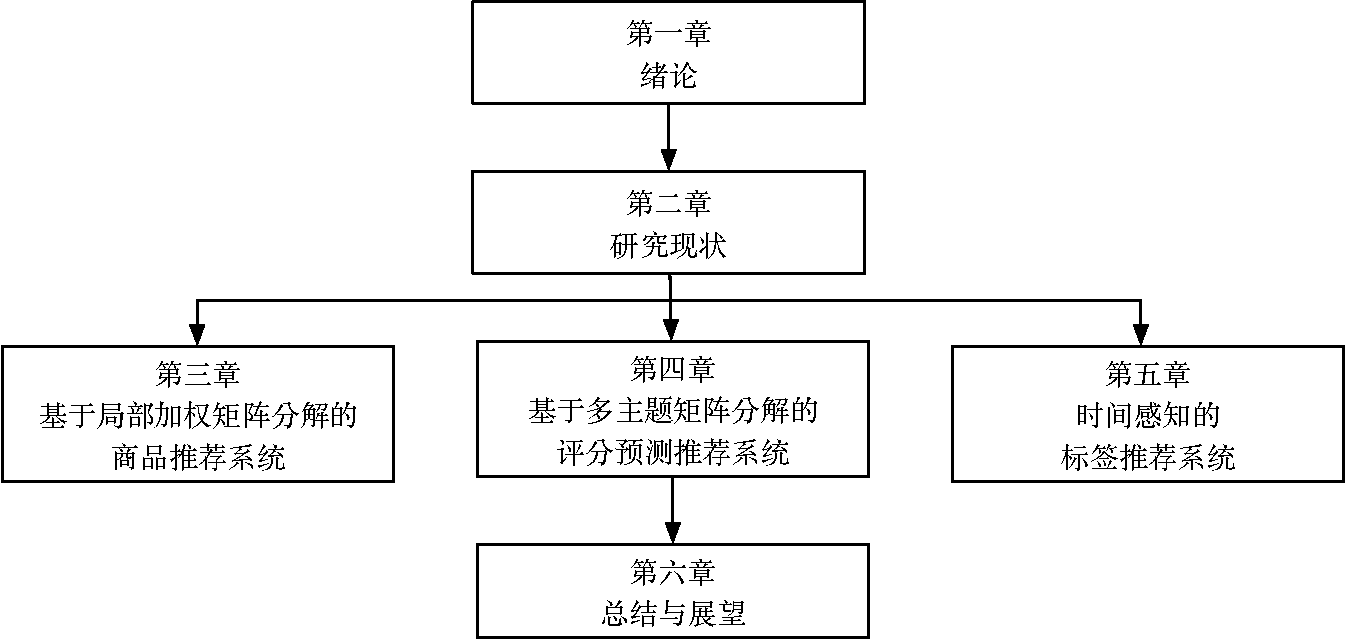
\includegraphics[width=1.05\textwidth]{Fig/chapter1/structure}
%	\caption{本文的组织结构}
%	\label{fig-chapter1-structure}
%\end{figure}
本文一共分为六章,章节安排如图~\ref{fig-chapter1-structure}所示:
\begin{itemize}
	\item 第二章从轨迹数据存储、轨迹降维以及轨迹数据相似性查询三个方面介绍了研究背景知识和研究现状。
	\item 第三章介绍了两个通用查询处理框架FTB和FLB以分别应对能同时提供上、下界的和仅能提供下界的相似度准则。
	\item 第四章介绍了如何将欧式距离嵌入到FTB框架中,并提供高效的查询结果。
	\item 第五章介绍了如何将DTW距离嵌入到FLB框架中,并提供高效的查询结果。
	\item 第六章对上述已有工作进行了总结,并展望了未来的研究方向和内容。
\end{itemize}

\clearpage
\phantom{s}
\clearpage
\chapter{问题定义及研究现状}\label{chapter:relatedwork}
本章第一节首先对数据模型和要解决的查询问题进行了定义,然后从以下方面介绍了相关的研究工作:轨迹索引、轨迹降维、轨迹相似度度量、时间序列数据top-$k$查询,最后对本章内容进行小结。

\section{问题定义}\label{chapter-related-coll}
本文的研究目标是给定一条查询轨迹,从存储在若干远程结点中的轨迹中找出$k$条距离最短或相似度最高的轨迹。为此,本节首先介绍了轨迹数据模型,接着介绍了查询的定义。

\subsection{轨迹数据}
轨迹是描述移动对象移动行为的数据。通常来说,一条轨迹$T$可看做包含$n$个元素(即轨迹点)的有序序列。每个轨迹点$\vp$包含了时间、位置等维度的信息。因此轨迹可被形式化定义为如下:
\begin{define}[轨迹]
轨迹形式化表示为:$T=\{\bp_{0}, \bp_{1},\cdots, \bp_{n-1}\}$。
\begin{equation}
T=\{\bp_{0}, \bp_{1},\cdots, \bp_{n-1}\}
\end{equation}
其中$|T|=n$代表轨迹所包含的点数,即轨迹的长度。每个轨迹点$\bp$包含时间($t$)、位置($l$)等维度的信息。因而$|\bp|=d$称为轨迹的维度。此外轨迹中的点严格按时间升序排列,即$\forall i,j,0\le i\le j < n$则$\bp_{i}.t \le \bp_{j}.t$。
\end{define}

轨迹数据的来源多样且复杂。根据移动对象的划分可分为如下几类:
\begin{itemize}
	\item \textsf{人类活动轨迹数据:}该类数据分为主动式和被动式。主动式数据是人们主动利用移动定位设备分享或汇报自己的位置等信息。典型的有社交网络中的数据,用户提交位置获得服务的数据。被动式数据是人们无意间使用各种服务时所产生的轨迹数据。典型的有公交刷卡轨迹和手机的信令轨迹数据。

	\item \textsf{交通工具轨迹数据:}这类数据主要是交通工具使用车载GPS设备所产生的移动轨迹数据。例如,出租车、公交车的活动轨迹数据。
	
	\item \textsf{动物活动轨迹数据:}这类数据是为了研究动物生活、迁徙等行为和习惯而捕获的数据。
	
		\item \textsf{自然现象活动轨迹数据:}这类数据典型的有台风、冰山、海洋事件等的轨迹数据,用以探索自然现象的活动规律。
\end{itemize}

轨迹数据符合大数据时代的 3V 特征,即量大、实时、多样。轨迹数据采样由于受设备、采样频率等因素影响,数据质量较低且各个轨迹的采样间隔差异显著。
这些问题导致原始轨迹数据的可用性较低。因此,我们在进行轨迹数据分析前往往需要经过数据清理(data cleaning)、地图匹配(map mathching)、轨迹分段(trajectory segmentation)等预处理方式化为校准轨迹。校准轨迹数据能够通过数据管理技术进行轨迹索引以便有效地存取。因此,本文所处理的轨迹数据为预处理后的校准轨迹数据。这样的数据有如下特点:(i)采样频率一致;(ii)长度一致;(iii)位置精度高。
这为我们挖掘轨迹模式从而提炼有价值的知识提供了可靠保障。

\subsection{分布式k近邻轨迹查询}
轨迹数据往往是分布式采集并存储的。为此假设有$M$个远程结点,每个远程结点$i$包含轨迹数据集$TS_{i}$。那么整个分布式轨迹数据集$TS=\bigcup_{i=1}^{M} TS_{i}$。我们的目标是给定查询轨迹,从分布式存储的$TS$数据集中,找出与其距离最近的$k$条轨迹。下面我们将给出查询的形式化定义:
\begin{define}[分布式k近邻轨迹查询]
	该查询形式为query$({\cal Q}, TS,DM,k)$,其中$\cal Q$为给定查询轨迹,$TS$为分布式轨迹数据集, $DM$为距离度量准则以及$k$为返回结果集大小。查询的目标是返回满足如下条件的轨迹集$\cal S$:(1)${\cal S} \subseteq TS$;(2)$| {\cal S}|=k$;
	(3)$\forall {\cal C} \in {\cal S}, {\cal C}' \in {TS - \cal S}$,$DM({\cal Q},{\cal C}) \le DM({\cal Q},{\cal C}')$。
\end{define}

传统的集中式环境下$k$近邻轨迹查询相比,分布式场景下的查询不仅注重查询效率,而且尤其注重通信开销。这是由于分布式场景中,远程结点和协调者结点的带宽资源往往是有限的。高的通信开销,意味着用户可能要花费更多的金钱。因此,用户允许多花一点时间以达到降低通信开销的目的。

\section{轨迹降维}\label{sec-c2-reduction}
为降低数据传输开销,一个直观的想法就是先对轨迹进行降维,然后将降维后的数据发送给。

\section{轨迹索引}\label{sec-c2-index}


\section{轨迹相似度度量}\label{sec-c2-measures}

\section{时间序列top-$k$查询}\label{sec-c2-topk}






\clearpage
\phantom{s}
\clearpage
\chapter{基于局部加权矩阵分解的商品推荐}
\label{chapter-lwmf}
本章主要介绍针对隐式反馈数据上进行商品推荐的研究工作。首先,章节~\ref{sect-lwmf-intro}阐述本章的研究背景、研究问题、研究主要贡献等。其次,章节~\ref{sec-lwmf-lwmf}重点介绍本章提出的模型,包括模型框架、优化算法等。随后,章节~\ref{sec-lwmf-exp}分析基于公开真实世界数据集上的实验结果。最后小结本章商品推荐的研究内容。

\section{引言}
\label{sect-lwmf-intro}


\textit{商品推荐}是推荐系统中的主要任务,是根据用户的历史行为数据,刻画用户画像,帮助人们在海量商品中发现他们感兴趣的商品。而用户的历史数据中按照用户的行为分为显式反馈数据和隐式反馈数据。其中显式反馈数据指的是用户在访问商品(例如购买商品,观看电影,餐馆用餐等行为)之后对商品进行评分表达自己的满意程度,标注标签表达商品的特性以及进行文本评价表明自己的体验感受。而隐式反馈数据指的是用户访问商品之后行为产生的非显式反馈的数据。因为显式反馈数据需要用户额外花一些时间进行评价,所以用户产生的大部分数据都属于隐式反馈。本章主要研究在隐式反馈数据集上的\textit{商品推荐}。

隐式反馈数据中,对于用户访问过的商品,次数代表了用户对商品的感兴趣程度,可以作为正反馈样例。大多数用户未访问过商品的数据对学习用户特征也是有帮助的,一般可以作为负反馈样例,但是次数为0代表了两种情况:(1)用户对这类商品不感兴趣;(2)用户对这类商品感兴趣,但还未发现此类商品。因此Hu等人~\cite{hu2008collaborative}提出了加权矩阵分解(Weighted Matrix Fatorization,简称WMF),访问次数大于0的数据为正反馈样本,次数等于0的样本为负样本,而次数则以权重的形式加入矩阵分解中(访问次数越多,权重越大,说明访问次数大于0的数据为正反馈样本的概率越大)。具体地,WMF已经在章节~\ref{sec-related-wmf}详细阐述。因为WMF模型是将用户和商品投射到潜在的低维空间,所以它的一个前提假设是隐式反馈数据中次数数据矩阵是全局低秩的。最近,Lee等人\cite{lee2013local,lee2014local}认为显式评分数据不是全局低秩的,而局部评分矩阵是低秩,拥有局部信息,通过对评分矩阵中的局部子矩阵进行建模能够得到更好的评分预测效果。类似的工作还有WEMAREC~\cite{chen2015wemarec}。本文统称这类工作为局部矩阵分解。如图~\ref{fig-lwmf-lmf}所示,局部矩阵分解模型首先将原始矩阵划分为若干更小的子矩阵,每个子矩阵内的用户(商品)之间是相互关联的,用来表示矩阵内的局部结构,然后利用标准的矩阵分解模型将每个子矩阵的用户和商品投射到隐藏空间,最后利用加权平均求和来预测最终的评分值。因此局部矩阵分解模型就可以利用局部结构特征来获得比原始矩阵分解更好的低秩近似。

\begin{figure}
	\centering
	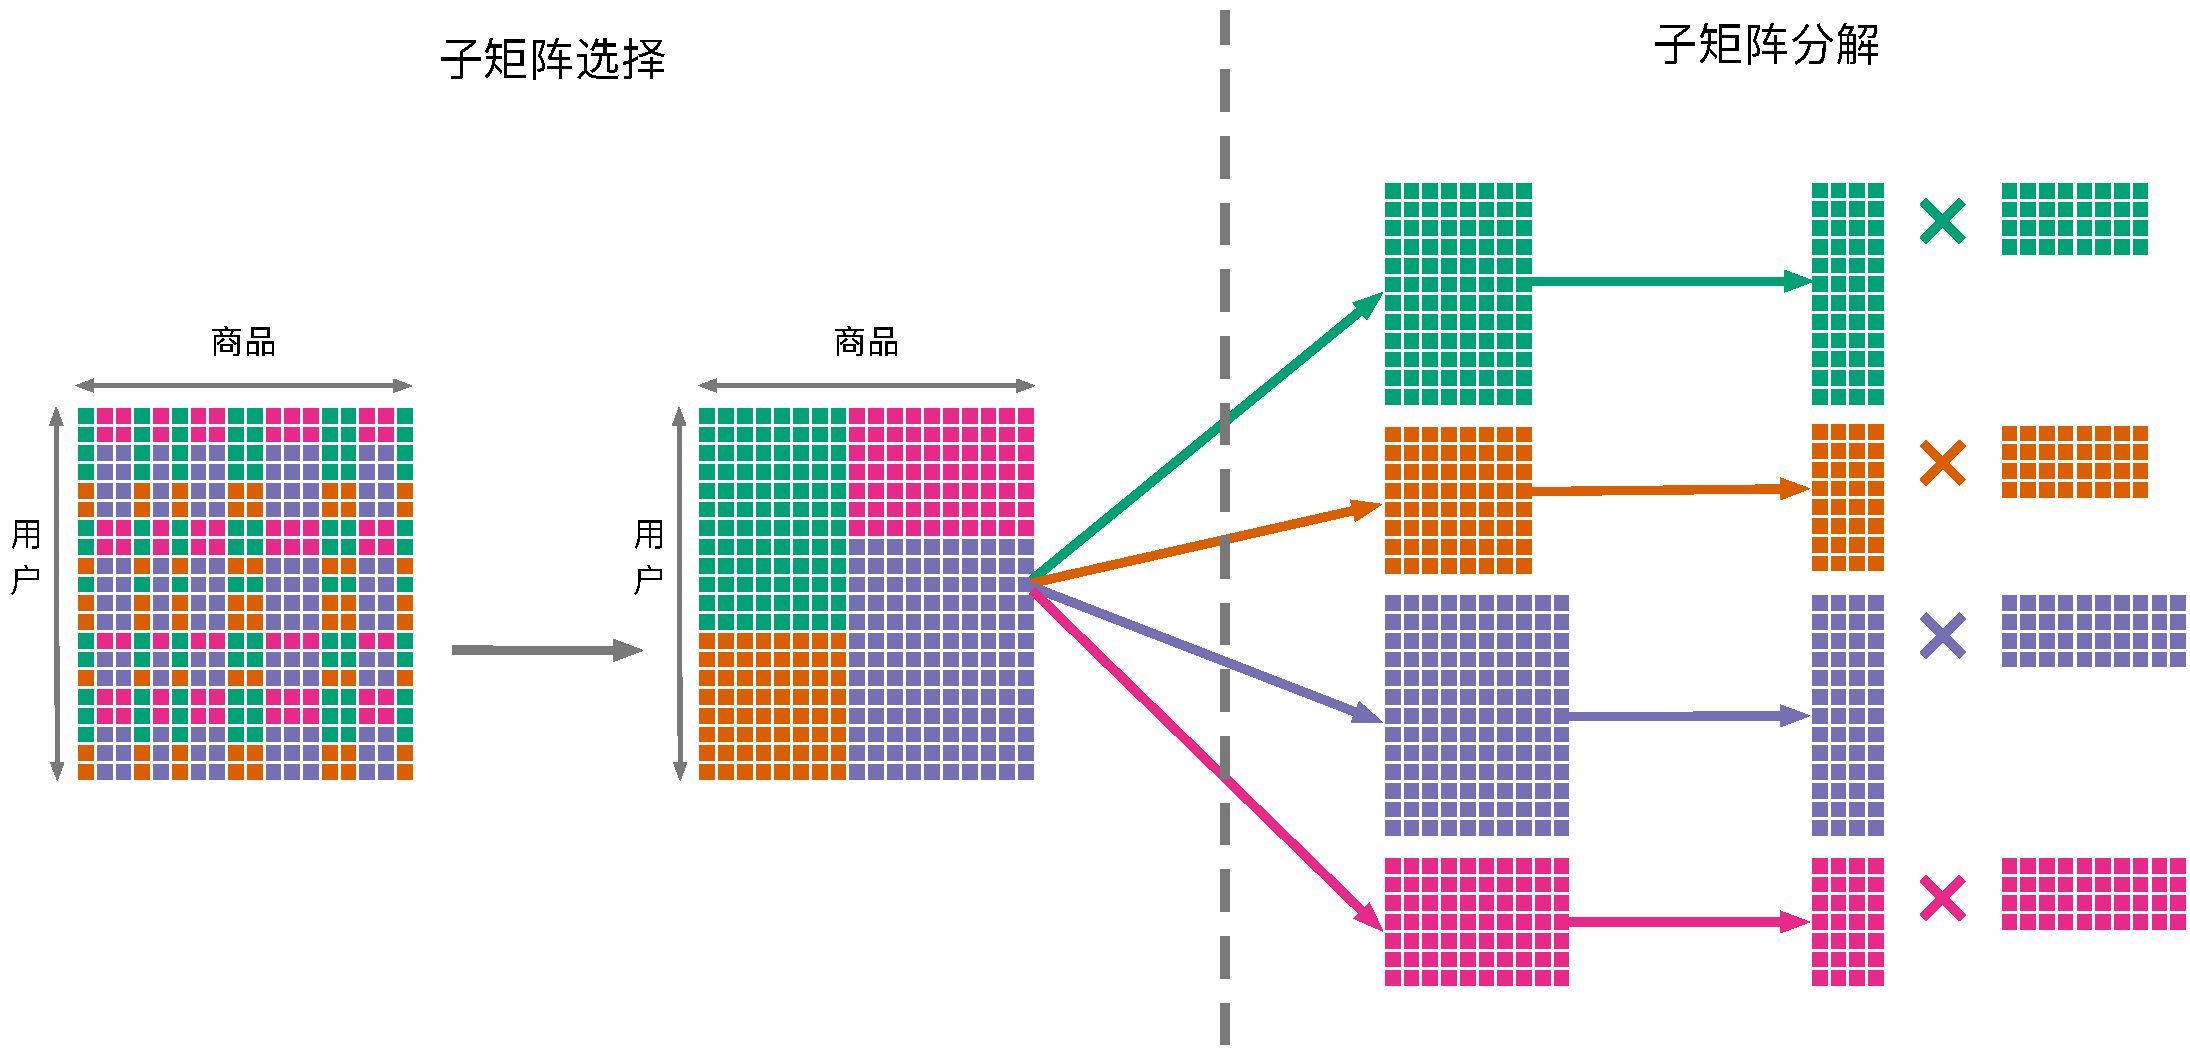
\includegraphics[width=1.0\textwidth]{Fig/lwmf/lmf}	
	\caption{局部矩阵分解模型}
	\label{fig-lwmf-lmf}
\end{figure}

考虑到隐式反馈数据和显式反馈数据的相似性,本章节也认为隐式反馈数据不是全局低秩的,而是局部低秩的,考虑在隐式反馈数据集上对数据的局部性质建模,进行个性化\textit{商品推荐}。例如,根据用户的签到数据集进行兴趣点(Point Of Interests,简称POI)推荐,因为兴趣点天然地具有地理信息这一特征,用户更倾向于访问与自身相近的地点,所以在同一个区域的用户访问的兴趣点比不在同一个区域的用户所访问的兴趣点更加类似。

因此,本章节设计了加权局部矩阵分解(Local Weighted Matrix Factorization,简称LWMF), 将LLORMA~\cite{lee2013local,lee2014local}和WMF~\cite{hu2008collaborative}相结合,使用核函数来寻找子矩阵和建立权重函数来建模用户局部偏好和商品的局部特性,提高商品推荐的准确率。这种方法也带来两个好处,(1)因为子矩阵的密度比原始矩阵要高很多,隐式数据中正反馈数据的稀疏性问题得到了一定程度的缓解;(2)子矩阵之间的分解可以并行进行,使得模型更加容易并行化。


具体地,本章主要贡献总结如下:
\begin{itemize}
	\item 本章节工作结合了LLORMA和WMF,提出了加权局部矩阵分解模型(LWMF),在隐式反馈数据上进行商品推荐。 LWMF通过将原始矩阵划分为子矩阵来对矩阵进行局部建模,并且缓解了访问次数数据的稀疏性问题以及使得矩阵分解模型更加容易并行化、分布式地进行模型训练。
	\item 为了更好地近似原始矩阵,本章节工作在基于核函数的方法上,提出DCGASC(折扣累积增益锚点集合覆盖)来选择子矩阵。同时,本章节工作还从理论上对DCGASC目标函数的次模性质和单调性进行分析,证明利用贪心算法能够以$1-\frac{1}{e}$得到近似最优解。
	\item 基于商品推荐问题,本章节⼯作进⼀步提出了两种变体方法:基于⽤户的 LWMF和基于商品的 LWMF,其中基于用户的LWMF对商品推荐更为合理,能够获得更好的性能。
	\item 本章节工作在真实数据集上进行充分的实验,在各个维度上比较了LWMF与WMF算法,实验结果表明了本章节模型的有效性。
\end{itemize}





\begin{table}
	\centering
	\caption{本章主要符号说明}
	\label{tab-lwmf-notation}%
	
	\begin{tabular}{cp{0.68\columnwidth}}
		\hline
		符号 & 符号描述 \bigstrut \\
		\hline\hline
		$\mathbf{R}^h$ & 第$h$个子数据矩阵 \bigstrut\\
		$\mathbf{C}^h$ &第$h$个01(二值化)化子数据矩阵  \bigstrut\\
		$ \mathbf{W}^h$ &01(二值化)化子数据矩阵$\mathbf{C}^h$的置信权重矩阵\bigstrut\\
		$ \mathbf{V}^h$ & 01(二值化)化子数据矩阵$\mathbf{C}^h$的子矩阵权重矩阵 \bigstrut\\
		$ \mathcal{P}^h$ &第$h$个数据子矩阵中的用户索引集合  \bigstrut\\
		$ \mathcal{Q}^h$ &第$h$个数据子矩阵中的商品索引集合  \bigstrut\\
		$ \mathbf{P}^h$  & 子数据矩阵$\mathbf{R}^h$中用户局部隐藏特征矩阵 \bigstrut\\
		$\mathbf{Q}^h$  & 子数据矩阵$\mathbf{R}^h$中商品局部隐藏特征矩阵 \bigstrut\\
		\hline
		$ \mathcal{\hat{A}}$ & 锚点集合($\subset \mathcal{A}$) \bigstrut\\
		$\hat{a}_h=\langle\hat{u}_h, \hat{m}_h\rangle$ & 锚点  ($\in \mathcal{\hat{A}}$)   \bigstrut\\
		$E(a_i, a_j)$ & 两个数据点之间的核函数值 \bigstrut\\
		$b$ & 核函数宽度参数 \bigstrut\\
		\hline
	\end{tabular}
\end{table}


\section{模型描述与优化}
\label{sec-lwmf-lwmf}
本章节首先介绍本章提出的针对隐式反馈数据的\textit{商品推荐}模型,称为局部加权矩阵分解(Local Weighted Matrix Factorization ,简称LWMF)。随后,本章设计了一个启发式的算法去选择子矩阵,提取数据矩阵的局部信息。最后,为了学习局部隐藏特征矩阵$\mathbf{P}^h$和$\mathbf{Q}^h$,本章还改进了交替最小二乘优化算法以适用于LWMF参数的快速学习。表\ref{tab-lwmf-notation}中列出了本章节中使用的符号表。基础的符号描述见表\ref{tab-basic-notation}中所示。矩阵和集合的字符的小写上标,例如$\mathbf{R}^h$和$\mathcal{P}^h$,表示不同的子矩阵以及相应用户索引集合。

\subsection{模型概览}
类似于LLORMA~\cite{lee2013local,lee2014local},LWMF模型首先从原始数据矩阵选择子矩阵,然后利用WMF对子矩阵进行矩阵分解。具体的WMF模型见章节\ref{sec-related-wmf}。本章结合了LLORMA和WMF在隐式反馈数据集上进行\textit{商品推荐},提出了局部加权矩阵分解,利用WMF对第$h$个二值化数据子矩阵$\mathbf{C}^h$进行如下分解:

\begin{equation}
\min_{\mathbf{P}_h,\mathbf{Q}_h}\sum_{u=1}^{N}\sum_{m=1}^{M}\mathbf{V}_{um}^h\mathbf{W}_{um}^h(\mathbf{C}_{um}^h-{\mathbf{P}_{u}^h}^\top \mathbf{Q}_{m}^h)^2+\lambda_\mathbf{P}^h\|\mathbf{P}^h\|_F^2+\lambda_\mathbf{Q}^h\|\mathbf{Q}^h\|_F^2
\end{equation}
其中$\lambda_\mathbf{P}^h$和$\lambda_\mathbf{Q}^h$ 是子矩阵用户和商品的正则化因子。原始二值化数据矩阵$\mathbf{C}$可以被一系列子矩阵集合$\mathcal{C}= \{\mathbf{C}^1,\mathbf{C}^2,...,\mathbf{C}^H\}$所组成:

\begin{equation}
\mathbf{C}_{um} \approx \frac{1}{\mathbf{Z}_{um}}\sum_{h=1}^H \mathbf{V}_{um}^h{\mathbf{P}^h_u}^\top \mathbf{Q}^h_m
\end{equation}
其中$\mathbf{Z}_{um} = \sum_{h=1}^H \mathbf{V}_{um}^{h}$是归一化因子,$\mathbf{V}^{h}_{um}$ 代表在子矩阵$\mathbf{C}^{h}$中项$\mathbf{C}^{h}_{um}$的权重。从上述公式可以看出,此类子矩阵集成分解的两个关键问题是(1) 如何选择和生成子矩阵?(2) 如何设置子矩阵的权重和根据子矩阵近似原始矩阵?

类似于LLORMA的子矩阵选择方法,本章节工作首先在数据集合$\mathcal{A}=\{a_1, a_2, ..., a_{|\mathbf{R}|}\}$ 中找一个数据点$a_i=\langle u_i, m_i \rangle$作为锚点$\hat{a}_h=\langle\hat{u}_h, \hat{m}_h\rangle$。然后利用相似度计算方法或者核函数计算锚点和其他数据点之间的相关程度。最后,选择那些相关程度大于一定常数的数据点组成子矩阵。可以看出,子矩阵中的数据点之间是相似的。另外,只要使用上述方法选择更多的锚点,从而得到更多的子矩阵。

实际上,本章工作使用Epanechnikov核函数去计算两个数据点$a_i=(u_i,m_i)$和$a_j = (u_j,m_j)$之间的相关程度。具体地,本章利用Epanechnikov核函数计算用户之间的相关程度和商品之间的相关程度,然后将它们的乘积作为数据点$a_i=(u_i,m_i)$和$a_j = (u_j,m_j)$之间的相关程度,具体如下表示:

\begin{eqnarray}
\mathit{E}(a_i, a_j)=\mathit{E_{b}}(u_i, u_j)\times\mathit{E_{b}}(m_i, m_j)
\end{eqnarray}
其中$\mathit{E_{b}}(u_i, u_j)$和$\mathit{E_{b}}(m_i, m_j)$是Epanechnikov核函数,

\begin{eqnarray}
	\mathit{E_{b}}(u_i, u_j)&\varpropto&(1-d(u_i,u_j)^2) \,\mathbf{1}_{\{d(u_i,u_j)\leq {b}\}}\nonumber\\
	\mathit{E_{b}}(m_i, m_j)&\varpropto&(1-d(m_i,m_j)^2) \,\mathbf{1}_{\{d(m_i,m_j)\leq {b}\}}\nonumber
\end{eqnarray}
其中$b$是核函数的宽度参数。两个用户(或者商品)的距离利用两个用户(或者商品)的隐藏特征向量计算。初始的用户隐藏特征向量和商品隐藏特征向量从数据矩阵$\mathbf{R}$中利用WMF中学习得到。对应地,本章工作利用$d(u_i, u_j)=arccos(\frac{\mathbf{P}_{u_i}\cdot \mathbf{P}_{u_j}}{\|\mathbf{P}_{u_i}\|\cdot\|\mathbf{P}_{u_j}\|})$ 计算用户$u_i$和$u_j$之间的距离,其中$\mathbf{P}_{u_i}$, $\mathbf{P}_{u_j}$就是第$u_i$个用户和第$u_j$个用户的全局隐藏特征向量。同理,使用同样的方法计算商品之间的距离。因此在选定锚点$\hat{a}_h=\langle\hat{u}_h, \hat{m}_h\rangle$ 的前提下,本章工作在子矩阵$\mathbf{R}^h$中设置用户商品对$\langle u_j,m_j \rangle$的权重为$\mathbf{V}^h_{u_jm_j} = \mathit{E}(\hat{a}_h, a_j)$ ,同时子矩阵的正则化参数变为$\lambda_\mathbf{P}^h = \lambda_\mathbf{P} \mathit{E_{b}}(\hat{u}_h, u_j)$和 $\lambda_\mathbf{Q}^h=\lambda_\mathbf{Q} \mathit{E_{b}}(\hat{m}_h, m_j)$。

从上述选择子矩阵的方法可以看出,每选出一个锚点就代表一个子矩阵。选择子矩阵集合$\mathcal{C}$实际上就是选择一个锚点集合$\hat{\mathcal{A}}=\{\hat{a}_1, \hat{a}_2, ..., \hat{a}_H\}$。 具体地,将在下一小节讨论选择锚点集合的算法。

\subsection{锚点集合选择}
\label{sec-lwmf-asc}
直观地,子矩阵集合$\mathcal{C}= \{\mathbf{C}^1,\mathbf{C}^2,...,\mathbf{C}^H\}$ 应该需要覆盖整个原始二值化矩阵$\mathbf{C}$,也就是说$\mathbf{C} = \cup_{\mathbf{C}^h\in \mathcal{C}}\mathbf{C}^h $。因此那些能够覆盖原始矩阵的子矩阵集合$\mathcal{C}$ 一般能够比不能覆盖原始矩阵的子矩阵集合更好地近似原始矩阵$\mathbf{C}$ 。因此,锚点集合选择问题就变成锚点集合覆盖问题。

\subsubsection{简单锚点集合覆盖}
\label{sec-lwmf-nasc}
本章节将所有非零用户-商品对,也就是所有数据点集合$\mathcal{A}=\{a_1,a_2,...,a_{|\mathbf{R}|}\}$作为锚点候选点集合。每个候选点$a_i$能够覆盖自己和一些其他候选点,表示为$\mathcal{A}^i=\{a_i, a_{i1}, a_{i2},..., a_{iD}\}\subset \mathcal{A}$。因此,类似于集合覆盖,本小节提出一个简单锚点集合覆盖方法,简称为锚点集合覆盖(Anchor point Set Cover problem, ASC),返回如下锚点集合
$\hat{\mathcal{A}} \subset \mathcal{A}$:

\begin{eqnarray}
\max J(\hat{\mathcal{A}})=|\cup_{i\in \hat{\mathcal{A}}}\mathcal{A}^i| \nonumber \\
s.t. |\hat{\mathcal{A}}| = H
\end{eqnarray}
显然, ASC问题是符合次模性质和单调性~\cite{guillory2010interactive}。因此,简单的贪心算法即可得到$1-\frac{1}{e}$ 的近似最优解。

\subsubsection{折扣累积收益锚点集合覆盖}
然而锚点集合覆盖中,一个前提假设是数据点被覆盖之后如果再次被覆盖就没有收益。但本章节工作认为覆盖训练数据点的过程中,在被覆盖一次之后的覆盖也是对最终推荐也有帮助的,但随着数据点被覆盖的次数越多,收益递减。这种情况类似于在信息检索中排序质量评测方法,例如归一化折扣累积收益 (Normalized Discounted Cumulative Gain, 简称NDCG)~\cite{jarvelin2002cumulated,clarke2008novelty}和期望排序倒数~(Expected Reciprocal Rank, 简称ERR) \cite{chapelle2009expected}。NDCG和ERR的主要思想是如果相关程度比较高的结果排到了后面,那么在统计收益时,对收益大小根据位置的前后打折扣。从这个折扣思路学习,本章节工作提出了一种启发式算法去建模这种锚点选择情况,称之为折扣累积收益锚点集合覆盖(Discounted Cumulative Gain Anchor Point Set Cover, 简称DCGASC)。DCGASC在每次数据点被覆盖时都获得覆盖收益,但是收益随着被覆盖次数的增多而递减。具体地,通过最大化如下目标函数返回一个锚点排序列表$\hat{\mathcal{A}} = \{\hat{a}_{1},\hat{a}_{2},...,\hat{a}_{H}\} \subset \mathcal{A}$:

\begin{align}
\label{equ-lwmf-dcgasc}
&\max J(\hat{\mathcal{A}}) \sum_{h=1}^{H}\sum_{a_l \in \hat{\mathcal{A}}^{h}}\alpha^{o_{lh}-1}(1-max_{h'\in\{1,...,h-1\}} E_b(\hat{a}_{h}, \hat{a}_{h'})) \nonumber \\
&\ \ \ \ \ \ \ \ \ \ \ \ \ \ \ \ \ \ \ \ \ \ \ \ \ \ \ \ \ \ \ \ \ \ \ \ \ \ \ \ \ \ \ \ \ \ \ \ s.t. |\hat{\mathcal{A}}| = H
\end{align}
其中$o_{lh}$代表数据点$a_l$被已选择的锚点$\{\hat{a}_1,\hat{a}_2,...,\hat{a}_h\}$覆盖的次数,$\alpha \in (0,1)$则是折扣系数。当数据点$a_l$之前已经被一个锚点覆盖,那么下次该数据点被覆盖时覆盖收益将会减少。当折扣系数$\alpha = 0$时,这个问题简化为简单锚点集合覆盖问题,详见小节~\ref{sec-lwmf-nasc}。当$\alpha = 1$时,该问题解就变成每次选择覆盖其他数据点最多的锚点。项$(1-max_{h'\in\{1,...,h-1\}} E_b(\hat{a}_{h}, \hat{a}_{h'}))$则表示DCGASC倾向于选择那些远离已经选择过的锚点,即与已选择过的锚点不相似的数据点。可以证明的是,目标函数$J(\cdot)$符合次模性质和单调性。

\begin{theorem}
	\label{theorem:submodular}
	DCGASC目标函数~\ref{equ-lwmf-dcgasc}是次模的,同时也是单调非减的。
\end{theorem}

\begin{proof}
假设$\mathcal{S}=\{\hat{a}_1,\hat{a}_2,...,\hat{a}_{H-1}\}$ ,$\mathcal{V}=\{\hat{a}_1,\hat{a}_2,...,\hat{a}_{H-1},..., \hat{a}_{X-1}\}$ 都是锚点集合,同时$X\geq H$ ,以及$a_i = {\hat{a}_X} \in \mathcal{A} \backslash \mathcal{V}$是下一个选择的锚点。 我们有:

\begin{align}
J(\mathcal{V}&\cup \{\hat{a}_X\})-J(\mathcal{V}) \nonumber \\
= &\sum_{h=1}^{X}\sum_{a_l \in \hat{\mathcal{A}}^{h}}\alpha^{o_{lh}-1}(1-max_{h'\in\{1,...,h-1\}} E_b(\hat{a}_{h}, \hat{a}_{h'})) \nonumber \\
- &\sum_{h=1}^{X-1}\sum_{a_l \in \hat{\mathcal{A}}^{h}}\alpha^{o_{lh}-1}(1-max_{h'\in\{1,...,h-1\}} E_b(\hat{a}_{h}, \hat{a}_{h'})) \nonumber \\
= &\sum_{a_l \in \mathcal{\hat{A}}^X}\alpha^{o_{lX}-1}(1-max_{h'\in\{1,...,X-1\}} E_b(\hat{a}_X, \hat{a}_{h'}))\geq 0
\end{align}
所以DCGASC目标函数~\ref{equ-lwmf-dcgasc}是单调非减的。

\begin{align}
\label{eq-marg}
J(\mathcal{S}&\cup \{\hat{a}_X\})-J(S)-(J(\mathcal{V}\cup \{\hat{a}_X\})-J(\mathcal{V}))\nonumber\\
&=\sum_{a_l \in \mathcal{\hat{A}}^X}\alpha^{o_{lX'}-1}(1-max_{h'\in\{1,...,H-1\}} E_b(\hat{a}_X, \hat{a}_{h'}))\nonumber\\
&-\sum_{a_l \in \mathcal{\hat{A}}^X}\alpha^{o_{lX}-1}(1-max_{h'\in\{1,...,X-1\}} E_b(\hat{a}_X, \hat{a}_{h'}))
\end{align}
其中$o_{lX'}$代表数据点$a_l$被锚点集合$S\cup \{\hat{a}_X\}$覆盖的次数。因为锚点集合覆盖的数目满足$o_{lX'}\leqslant o_{lX}$,折扣系数$\alpha\in [0,1]$以及$max_{h'\in\{1,...,H-1\}} E_b(\hat{a}_{X},\hat{a}_{h'})\leq \max_{h'\in\{1,...,X-1\}} E_b(\hat{a}_{X},\hat{a}_{h'})\leq 1$,可以得出$J(\mathcal{S}\cup \{\hat{a}_X\})-J(\mathcal{S})-(J(\mathcal{V}\cup \{\hat{a}_X\})-J(\mathcal{V}))\geq0$。所以DCGASC目标函数~\ref{equ-lwmf-dcgasc}是次模的。

综上所述,DCGASC目标函数~\ref{equ-lwmf-dcgasc}是次模的,同时也是单调非减的。
\end{proof}

因为DCGASC目标函数的单调性和次模性,本章节工作能够简单地使用贪心算法可以得到 $1-\frac{1}{e}$ 的近似最优解保证~\cite{nemhauser1978analysis}。算法~\ref{algo-wpitf-dcgasc}展示了这个贪心算法:第1和2行首先将能够覆盖其他数据点最多的数据点作为锚点,然后3-5行使用公式~\ref{eq-marg}依次得到接下来的$(H-1)$个锚点。

 \begin{algorithm}
	\begin{algorithmic}[1]
		\caption{DCGASC贪心算法}
		\label{algo-wpitf-dcgasc}
		\REQUIRE{数据点集合$\mathcal{A}$,锚点数量$H$, DCGASC函数$J$和被数据点$a_i$覆盖的数据点集合$A^i$;}
		\ENSURE{锚点列表$\hat{\mathcal{A}} \subseteq \mathcal{A}$,其中$|\hat{\mathcal{A}}| = H$;}
		
		\STATE {$\hat{a}_1 \leftarrow \arg \max_{a_i \in \mathcal{A}} |\mathcal{A}^i|$;}
		\STATE 	{$\hat{\mathcal{A}} \leftarrow \{\hat{a}_1\} $;}
		
		\FOR{$h=2:H$} 
			\STATE {$\hat{a}_h \leftarrow \arg \max_{a_i' \in \mathcal{A} \setminus \hat{\mathcal{A}}}f(\hat{\mathcal{A}} \cup \{a_i'\}) - f(\hat{\mathcal{A}})$;}
			\STATE {$\hat{\mathcal{A}} \leftarrow \hat{\mathcal{A}}\cup \{\hat{a}_h\}$;	}
		\ENDFOR
		
		\RETURN{$\hat{\mathcal{A}}$;}
	\end{algorithmic}
\end{algorithm}

\subsection{优化算法}
\label{sec-lwmf-opt}
交替最小二乘算法(Alternating Least Square,简称ALS)是一种优化加权矩阵分解的流行算法~\cite{hu2008collaborative}。不同于原始的ALS,He等人\cite{he2016fast}提出快速元素级交替最小二乘学习算法。该算法通过固定隐藏特征向量中其他维度数值,优化每维坐标数值,同时通过基于商品消费次数对缺失值引入对应权重,避免大量的重复计算,从而加速计算、学习参数,使得参数学习效率提高K倍且有相似的推荐效果。本章节使用元素级交替最小二乘算法学习子矩阵隐藏特征向量,并利用子矩阵数据点权重的计算方法,对元素级交替最小二乘做了类似于文章\cite{he2016fast}的加速优化,使得能够较快地学习子矩阵隐藏特征向量。具体地,子矩阵$\mathbf{R}^h$中第$u$个用户隐藏特征向量的基本迭代公式如下:

\begin{equation}
\label{eq-p_update1}
\mathbf{P}_{uk}^h = \frac{\sum_{m\in \mathcal{M}^h}(\mathbf{C}_{um}-\mathbf{\hat{C}}_{um,k}^h)\mathbf{V}_{um}^h\mathbf{W}_{um}\mathbf{Q}_{mk}^h}{\sum_{m\in \mathcal{M}^h}\mathbf{V}_{um}^h\mathbf{W}_{um}\mathbf{Q}_{mk}^h\mathbf{Q}_{mk}^h+\lambda_\mathbf{P}^h}
\end{equation}
其中, $\mathcal{M}^h$表示子矩阵$\mathbf{R}^h$存在于原始矩阵$\mathbf{R}$的商品索引集合,$\mathbf{\hat{C}}_{um,k}^h$表示需要更新坐标的隐藏特征向量的预测值,也就是$\mathbf{\hat{C}}_{um,k}^h = \mathbf{\hat{C}}_{um}^h-\mathbf{P}_{uk}^h\mathbf{Q}_{mk}^h$($\mathbf{\hat{C}}_{um}^h$表示预测值)。可以注意到全局二值化拟合矩阵$\mathbf{C}_{um}$和置信权重矩阵$\mathbf{W}_{um}$在不同的子矩阵中都是一样的。同时相应的子矩阵权重$\mathbf{V}_{um}^h$在公式~\ref{eq-p_update1}中是和原始WMF唯一不同的项,导致不能对公式~\ref{eq-p_update1}进行直接使用类似于工作~~\cite{hu2008collaborative}和工作~\cite{he2016fast}的加速计算。幸运地是,因为$\mathbf{V}_{um}^h$的计算方式是由用户和商品组成,即$\mathbf{V}^h_{um} = \mathit{E_{b}}(\hat{u}_h, u)\times\mathit{E_{b}}(\hat{m}_h, m)$ ,而且正则化系数也是有用户和商品权重成份($\lambda_\mathbf{P}^h = \lambda_\mathbf{P}\mathit{E_{b}}(\hat{u}_h, u)$),因此通过分子分母约分,然后计算中间结果,仍然可以达到类似于工作~\cite{he2016fast}加速学习参数的效果。首先,项$\mathit{E_{b}}(\hat{u}_h, u)$ 在公式~\ref{eq-p_update1}中分子和分母是同时存在的,因此可以约分消去项$\mathit{E_{b}}(\hat{u}_h, u)$。而且可以发现如果$\mathit{E_{b}}(\hat{u}_h, u)=0$,那么在子矩阵权重为0,子矩阵分解中不需要计算它的局部隐藏特征向量。这里,本章工作首先聚焦于分子部分的计算:

\begin{align}
\label{equ-lwmf-fenzi}
\sum_{m\in \mathcal{Q}^h}&(\mathbf{C}_{um}-\mathbf{\hat{C}}_{um,k}^h)\mathit{E_{b}}(\hat{m}_h, m)\mathbf{W}_{um}\mathbf{Q}_{mk}^h \nonumber \\
=&\sum_{m\in \mathcal{Q}_u^h}[\mathbf{W}_{um}\mathbf{C}_{um}-(\mathbf{W}_{um}-1)\mathbf{\hat{C}}_{um,k}^h]\mathit{E_{b}}(\hat{m}_h, m)\mathbf{Q}_{mk}^h\nonumber \\
-&\sum_{m\in \mathcal{Q}^h}\mathit{E_{b}}(\hat{m}_h, m)\mathbf{\hat{C}}_{um,k}^h\mathbf{Q}_{mk}^h
\end{align}
其中$\mathcal{Q}_u^h$代表的是第$u$个用户在子矩阵$\mathbf{R}^h$中消费的商品集合。因为对于任何一个用户项$\mathit{E_{b}}(\hat{m}_h, m)$都是一样的,所以在公式~\ref{equ-lwmf-fenzi}中可以使用缓存的方法。项$\sum_{m\in \mathcal{Q}^h}\mathit{E_{b}}(\hat{m}_h, m)\mathbf{\hat{C}}_{um,k}^h\mathbf{Q}_{mk}^h$通过交换律可以加速运算:

\begin{equation}
\sum_{m\in \mathcal{Q}^h}\mathit{E_{b}}(\hat{m}_h, m)\mathbf{\hat{C}}_{um,k}^h\mathbf{Q}_{mk}^h 
= \sum_{f\neq k}\mathbf{P}_{uf}\sum_{m\in \mathcal{Q}^h}\mathit{E_{b}}(\hat{m}_h, m)\mathbf{Q}_{mk}^h\mathbf{Q}_{mf}^h
\end{equation}

因此,在进行学习局部用户隐藏特征向量时,项$\sum_{m\in \mathcal{Q}^h}\mathit{E_{b}}(\hat{m}_h, m)\mathbf{Q}_{mk}^h\mathbf{Q}_{mf}^h$是可以提前计算好的,然后用于学习所有用户的局部隐藏特征向量。相似地,也可以将相同的方法运用在公式~\ref{eq-p_update1}中分母的计算。本章节定义局部商品缓存矩阵变量$\mathbf{S}^{\mathbf{Q}^h}$,令它为$\mathbf{S}^{\mathbf{Q}^h}=\sum_{m\in \mathcal{Q}^h}\mathit{E_{b}}(\hat{m}_h, m)\mathbf{Q}_m^h\mathbf{Q}_m^{h\top}$,那么公式~\ref{eq-p_update1}就可以变为如下计算:

\begin{align}
\label{eq-p_update2}
\mathbf{P}_{uk}^h =& \{\sum_{m\in \mathcal{Q}_u^h}[\mathbf{W}_{um}\mathbf{C}_{um}-(\mathbf{W}_{um}-1)\mathbf{\hat{C}}_{um,k}^h]\mathit{E_{b}}(\hat{m}_h, m)\mathbf{Q}_{mk}^h
-\sum_{f\neq k}\mathbf{P}_{uf}^h\mathbf{S}^{\mathbf{Q}^h}_{fk}\}\nonumber\\&/\{\sum_{m\in \mathcal{Q}^h_u}\mathit{E_{b}}(\hat{m}_h, m)(\mathbf{W}_{um}-1)\mathbf{Q}_{mk}^h\mathbf{Q}_{mk}^h+\mathbf{S}^{\mathbf{Q}^h}_{kk}+\lambda_\mathbf{P}\}
\end{align}
其中项$\mathbf{S}^{\mathbf{Q}^h}_{fk}$是缓存矩阵$\mathbf{S}^{\mathbf{Q}^h}$的第$f$行第$k$列元素。

相似地,定义局部用户缓存矩阵变量$\mathbf{S}^{\mathbf{P}^h}$,令其为$\mathbf{S}^{\mathbf{P}^h}=\sum_{u\in \mathcal{P}^h}\mathit{E_{b}}(\hat{u}_h, u)\mathbf{P}_u^h\mathbf{P}_u^{h\top}$,那么局部商品隐藏特征变量迭代公式如下表示:

\begin{align}
\label{eq-q_update2}
\mathbf{Q}_{mk}^h = &\{\sum_{u\in \mathcal{P}_m^h}[\mathbf{W}_{um}\mathbf{C}_{um}-(\mathbf{W}_{um}-1)\mathbf{\hat{C}}_{um,k}^h]\mathit{E_{b}}(\hat{u}_h, u)\mathbf{P}_{uk}^h
-\sum_{f\neq k}\mathbf{Q}_{mf}^h\mathbf{S}^{\mathbf{P}^h}_{fk}\}\nonumber\\&/\{\sum_{u\in \mathcal{P}^h_m}\mathit{E_{b}}(\hat{u}_h, u)(\mathbf{W}_{um}-1)\mathbf{P}_{uk}^h\mathbf{P}_{uk}^h+\mathbf{S}^{\mathbf{P}^h}_{kk}+\lambda_\mathbf{Q}\}
\end{align}

在子矩阵$\mathbf{R}^h$每轮用户局部隐藏特征向量学习迭代中,计算缓存矩阵变量$\mathbf{S}^{\mathbf{Q}^h}$的复杂度为$O(|\mathcal{Q}^h|K^2)$,学习每个用户的局部隐藏特征向量的复杂度为$O(|\mathbf{R}^h|K)$,其中$|\mathcal{Q}^h|$代表集合$\mathcal{Q}^h$的大小,$|\mathbf{R}^h|$代表的是子矩阵$\mathbf{R}^h$非零元素的个数。同理,子矩阵$\mathbf{R}^h$每轮商品局部隐藏特征向量学习迭代的复杂度为$O(|\mathcal{P}^h|K^2+|\mathbf{R}^h|K)$。假设原始矩阵$\mathbf{R}$被$H$个子矩阵覆盖,每个非零元素覆盖的次数为$\hat{H}$,那么有$\hat{H}|\mathbf{R}|=\sum_{h=1}^{H}|\mathbf{R}^h|$,因此整个LWMF模型每一轮迭代的复杂度为$O(\hat{H}(NK^2+MK^2+|\mathbf{R}|K))$,是全局加权矩阵分解复杂度的$\hat{H}$倍。

 \begin{algorithm}
	\begin{algorithmic}[1]
		\caption{LWMF优化算法}
		\label{algo-lwmf-learning}
		\REQUIRE{$<$用户,商品,次数$>$数据矩阵$\mathbf{R}$,锚点数量$H$,DCGASC函数$J$, 被数据点$a_i$覆盖的集合$\mathcal{A}^i$,权重矩阵$\mathbf{W}$,正则化系数$\lambda_\mathbf{P}$和$\lambda_\mathbf{Q}$,隐藏特征向量维度$K$;}
		\ENSURE{用户局部隐藏特征矩阵$\{\mathbf{P}^1,\mathbf{P}^2,...,\mathbf{P}^H\}$,商品局部隐藏特征矩阵$\{\mathbf{Q}^1,\mathbf{Q}^2,...,\mathbf{Q}^H\}$和各个子矩阵权重$\{\mathbf{T}^1,\mathbf{T}^2,...,\mathbf{T}^H\}$;}
		
		\STATE {利用公式~\ref{equ-binarized-matrix}从原始数据矩阵$\mathbf{R}$计算二值化矩阵$\mathbf{C}$;}
		\STATE 	{使用元素级最小二乘算法~\cite{he2016fast}计算全局隐藏特征向量$\mathbf{P}$和$\mathbf{Q}$;}
		\STATE 	{使用DCGASC算法~\ref{algo-wpitf-dcgasc}得到锚点集合$\mathcal{\hat{A}}= \{\hat{a}_{1}, \hat{a}_{2},..., \hat{a}_{H}\}$;}
		
		\FOR{$h$ $\leftarrow$ $1$ to $H$} 
		
			\FOR{$u$ $\leftarrow$ $1$ to $N$}
				\IF{$E_b(\hat{u}_h, u)>0$}
					\STATE{$\mathcal{P}^h$ $\leftarrow$ $\mathcal{P}^h \cup \{u\}$;}
				\ENDIF
			\ENDFOR
			
			\FOR{$m$ $\leftarrow$ $1$ to $M$}
				\IF{$E_b(\hat{m}_h,m)>0$}
					\STATE{	$\mathcal{Q}^h$ $\leftarrow$ $\mathcal{Q}^h \cup \{m\} $;}
				\ENDIF
			\ENDFOR

			//更新局部用户隐藏特征向量
			\STATE {$\mathbf{S}^{\mathbf{Q}^h}=\sum_{m\in \mathcal{Q}^h}\mathit{E_{b}}(\hat{m}_h, m)\mathbf{Q}_m^h\mathbf{Q}_m^{h\top}$;}
			
			\FORALL{$u \in \mathcal{P}^h$}
			
				\FORALL{$m\in \mathcal{Q}_u^h$}
				 	\STATE{$\mathbf{\hat{C}}_{um}^h\leftarrow {\mathbf{P}_u^h}^\top \mathbf{Q}_m^h$;}
				\ENDFOR
				
				\FOR{$k$ $\leftarrow$ $1$ to $K$}
				
					\FORALL{$m\in \mathcal{Q}_u^h$}
						\STATE{$\mathbf{\hat{C}}_{um,k}^h\leftarrow\mathbf{\hat{C}}_{um}^h-\mathbf{P}_{uk}^h\mathbf{Q}_{mk}^h$;}
					\ENDFOR
				
					\STATE{利用公式~\ref{eq-p_update2}计算$\mathbf{P}_{uk}^h$;}
				
					\FORALL{$m\in \mathcal{Q}_u^h$}
						\STATE{$\mathbf{\hat{C}}_{um,k}^h\leftarrow\mathbf{\hat{C}}_{um}^h+\mathbf{P}_{uk}^h\mathbf{Q}_{mk}^h$;}
					\ENDFOR
				
				\ENDFOR
			\ENDFOR
			
			//更新局部商品隐藏特征向量

			\STATE {$\mathbf{S}^{\mathbf{P}^h}=\sum_{u\in \mathcal{P}^h}\mathit{E_{b}}(\hat{u}_h, u)\mathbf{P}_u^h\mathbf{P}_u^{h\top}$;}
			
			\FORALL{$m \in \mathcal{Q}^h$}
			
				\FORALL{$u\in \mathcal{P}_m^h$}
					\STATE{$\mathbf{\hat{C}}_{um}^h\leftarrow {\mathbf{P}_u^h}^\top \mathbf{Q}_m^h$;}
				\ENDFOR
			
				\FOR{$k$ $\leftarrow$ $1$ to $K$}
			
					\FORALL{$u\in \mathcal{P}_m^h$}
						\STATE{$\mathbf{\hat{C}}_{um,k}^h\leftarrow\mathbf{\hat{C}}^h_{um}-\mathbf{P}_{uk}^h\mathbf{Q}_{mk}^h$;}
					\ENDFOR
			
					\STATE{利用公式~\ref{eq-q_update2}计算$\mathbf{Q}_{mk}$;}
			
					\FORALL{$u\in \mathcal{P}_m^h$}
						\STATE{$\mathbf{\hat{C}}_{um,k}^h\leftarrow\mathbf{\hat{C}}^h_{um}+\mathbf{P}_{uk}^h\mathbf{Q}_{mk}^h$;}
					\ENDFOR
			
				\ENDFOR
			\ENDFOR
				
		\ENDFOR
		
		\RETURN{$\mathcal{P},\mathcal{Q}$;}
		
	\end{algorithmic}
\end{algorithm}

算法~\ref{algo-lwmf-learning} 概括了学习局部隐藏特征向量的过程。首先,本章工作使用快速元素级最小二乘法~\cite{he2016fast}学习全局隐藏特征向量$\mathbf{P}$和$\mathbf{Q}$,然后通过锚点选择算法DCGASC算法~\ref{algo-wpitf-dcgasc}获得$H$个锚点集合,利用Epanechnikov核函数计算得到$H$个子矩阵。最后使用改进的快速元素级最小二乘法学习每个子矩阵的局部隐藏特征矩阵。

\begin{figure}
	\centering
	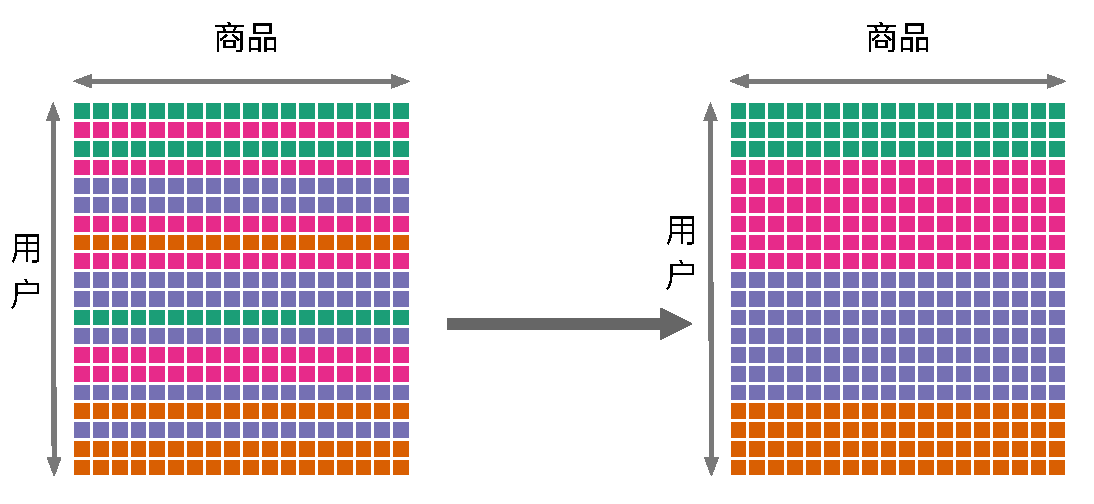
\includegraphics[width=0.75\textwidth]{Fig/lwmf/user}
	\caption{基于用户的局部矩阵分解模型}
	\label{fig-lwmf-user}
\end{figure}

\subsection{基于用户的局部加权矩阵分解}
上述的LWMF方法使用被选中的子矩阵去对\textit{局部}性质进行建模,而忽视了全局信息。特别对于商品推荐问题,应该考虑从所有商品中推荐用户感兴趣的商品。因此,本章节提出一种变种的LWMF方法-基于用户的局部加权矩阵分解,它仅仅从用户角度选择锚点,将所有商品放入子矩阵中。 给定用户集合$\mathcal{P}=\{u_1,u_2,...,u_N\}$ ,以及每个用户$u_i$能覆盖本身和其他一些用户,表示为$\bar{\mathcal{P}^i}=\{u_i, u_{i1}, u_{i2},..., u_{iD}\}$,需要找出一个用户锚点集合$\mathcal{\hat{P}}=\{\hat{u}_1,\hat{u}_2,...,\hat{u}_H\}$去最大化覆盖用户集合,目标函数如下:

\begin{align}
&\max J(\mathcal{\hat{P}}) \sum_{h=1}^{H}\sum_{u_l \in \bar{\mathcal{P}}^h}\alpha^{o_{lh}-1}(1-max_{h'\in\{1,...,h-1\}} E_b(\hat{u}_h,\hat{u}_{h'})) \nonumber \\
&\qquad\qquad\qquad\qquad\qquad\qquad\qquad\qquad\qquad\qquad s.t. |\mathcal{\hat{P}}| = H
\end{align}

显然地,这个基于用户的DCGASC目标函数也是符合次模性质和非减函数。图~\ref{fig-lwmf-user}展示了基于用户的LWMF模型去选择子矩阵的过程。因为不需要考虑商品,基于用户的LWMF会更快地选择用户锚点集合。而且,对于商品推荐来说,基于用户的LWMF模型也相对是比较合适的。作为对基于用户的LWMF模型的比较,本章节也加入了基于商品的LWMF模型,它仅仅考虑商品去选择锚点且把所有用户放入子矩阵中。



%\begin{figure}
%	\centering
%	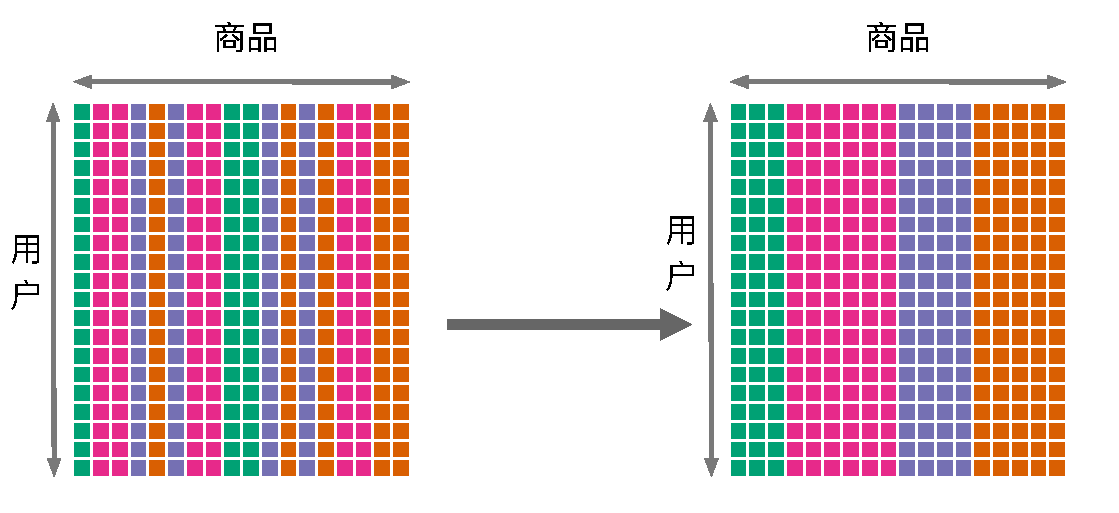
\includegraphics[width=0.7\textwidth]{Fig/lwmf/item}
%	\caption{基于商品的局部矩阵分解}
%	\label{fig-lwmf-item}
%\end{figure}

\section{实验及分析}
\label{sec-lwmf-exp}

本节将在真实世界的隐式反馈数据上评估本章节提出的模型。本小节首先介绍所使用的真实世界数据集和实验设置。随后实验在特定参数下和其他一些著名\textit{商品推荐}模型进行比较,特别是全局的WMF模型。最后实验中也进行了不同锚点数量(也就是不同数量的子矩阵)和不同锚点选择方法下推荐结果的比较。

\subsection{实验设置}
\subsubsection{数据集}
本章工作在实验中选择论文\cite{yuan2013time}中的两个真实世界数据集。一个是新加坡2010年8月到2011年7月的Foursquare签到数据,另外一个是加利福利亚州和内华达州2009年2月到2010年10的签到数据。这两个数据都是非常流行的在线移动位置服务数据,只有签到数据,但没有用户的喜好数据,是非常典型的用户隐式反馈数据。

Foursquare签到数据包含由2,312个用户,5,596个POIs组成的194,108个签到数据,稠密度是$1.50\times10^{-2}$。Gowalla签到数据包含由10,162个用户,24,238个POIs组成的456,967个签到数据,稠密度是$1.86\times10^{-3}$。两个数据集都比较稀疏。表\ref{tab-lwmf-stat}展示了两个数据集更详细的信息。另外,根据用户-地点-签到次数随机将80\%的数据集分割为训练集,剩下的20\%为测试集。对所有方法,本实验分别独立进行5次,最终5次实验的平均值作为最终推荐方法的结果。

\begin{table}
	\centering
	\caption{隐式反馈数据集Gowalla和Foursquare的详细信息}
	\begin{tabular}{|r||r|r|}
		\hline
		& Foursquare & Gowalla \bigstrut\\
		\hline
		\hline
		\#users & 2,321 & 10,162 \bigstrut\\
		\hline
		\#locations & 5,596 & 24,238 \bigstrut\\
		\hline
		\#check-ins & 194,108 & 456,967 \bigstrut\\
		\hline
		avg. \#users per loc. & 34.69 & 18.85 \bigstrut\\
		\hline
		avg. \#loc. per user & 83.63 & 44.97 \bigstrut\\
		\hline
		max \#users per loc. & 695   & 2,195 \bigstrut\\
		\hline
		max \#loc. per user & 311   & 1,113 \bigstrut\\
		\hline
	\end{tabular}%
	\label{tab-lwmf-stat}%
\end{table}%

\subsubsection{参数设置}

接下来,说明本实验中的参数设置。正则化参数$\lambda$设置为10,因为实验中发现该推荐效果对该正则化参数的设置不是非常敏感,10是一个相对较好的数值。置信权重矩阵$\mathbf{W}$中控制权重增量速率的参数$\varepsilon$在数据集Foursquare设置为2,另一个数据集Gowalla上设置为3。用来计算用户之间和商品之间的Epanechanikov核函数的带宽参数设置为$b=0.8$。另外本实验设置锚点选择方法DCGASC的折扣参数$\alpha$为0.4。折扣参数对推荐效果的影响后面有相应的实验结果进行说明。对两个数据集,本实验都选择100个锚点进行最后的矩阵分解。在实验中,可观察到随着锚点数量增多,也就是子矩阵数量增多,推荐效果越好,但是训练时间增加,并且推荐效果增强,收益却减少。实验经验表明100个锚点已经能够得到较好的推荐效果。

\subsubsection{评价标准}
对于评价指标,本实验使用精准率Precision@n和召回率Recall@n衡量模型的推荐性能。对第$u$个用户,本章假设符号$\mathcal{I}^P_u$为他的商品推荐列表,符号$\mathcal{I}^T_u$为该用户在测试数据集中的真实商品列表。Precision@n和召回率Recall@n分别表示为:

\begin{align}
Precision@n &= \frac{1}{N}\sum_{u=1}^{N}\frac{|\mathcal{I}^P_u\bigcap \mathcal{I}^T_u|}{n}\\
Recall@n &= \frac{1}{N}\sum_{u=1}^{N}\frac{|\mathcal{I}^P_u\bigcap \mathcal{I}^T_u|}{|\mathcal{I}^T_u|}
\end{align}
其中$|\mathcal{I}^P_u|$表示列表$\mathcal{I}^P_u$的大小,等于$n$。在基础实验中,选择$n=10$来评价实验结果。

\subsubsection{对比方法}
本实验总共比较7个隐式反馈数据推荐的模型:
\begin{itemize}
	\item MP:这是最基本方法,对目标用户推荐最流行的商品。 
	\item KNN$_u$: 这个是基于用户的协同过滤方法,利用训练集计算用户跟用户之间的相似度,求出$K$\footnote{这里的$K$指的是近邻数量,不是指局部隐藏特征向量的维度。}个最相似的用户对商品的评分之和作为最终预测值。
	\item KNN$_m$: 这个方法跟KNN$_u$类似,是基于商品的协同过滤方法,利用训练集中计算商品跟商品之间的相似度,根据目标用户对其他商品的评测值和跟目标商品之间的相似度计算预测值。特别地,我们设置两个$K$近邻方法的近邻数量为100。
	\item WMF: 该方法为现在最流行的隐式反馈数据top-n商品推荐方法\cite{hu2008collaborative,he2016fast},本文的方法也是基于该方法上提出的,它对缺失数据设置统一的权重,在整个数据集上进行隐藏特征向量参数学习优化。其他基本参数设置和上面参数设置说明一致。
	\item LWMF$_{both}$: 这个方法是本文提出的,利用核函数选择锚点,进而得到子矩阵,来对数据集的局部性质进行建模。
	\item LWMF$_u$: LWMF$_{both}$的一个变种,该方法仅仅考虑用户去选择锚点,并把所有商品放入子矩阵中。
	\item LWMF$_m$:  LWMF$_{both}$的另一个变种,该方法仅仅考虑商品去选择锚点,并把所有用户放入子矩阵中。
\end{itemize}

另外,本实验中也比较了两类不同的锚点选择方法,来研究锚点选择的不同对最终LWMF推荐效果的影响:
\begin{itemize}
	\item 随机选择: 利用均匀分布从训练集中随机选择锚点,和论文\cite{lee2013local,lee2014local}中锚点选择方法类似。
	\item 最大化折扣累积收益锚点集合覆盖锚点选择(DCGASC):利用最大化折扣累积收益锚点集合覆盖函数进行锚点选择。
\end{itemize}

因此LWMF根据锚点选择方法的不同也将分为两个子方法:{LWMF\_random}和{LWMF\_DCGASC}。默认地,不作特别说明,LWMF代表的模型是{LWMF\_DCGASC}方法。

\subsection{实验结果及分析}
本小节将具体介绍在Foursquare和Gowalla两个数据集上的实验结果,主要从以下四个方面进行讨论:
\begin{itemize}
	\item[1.]   各类不同推荐方法的对比;
	\item[2.]  不同锚点数量(即不同子矩阵个数)对本文模型LWMF最终推荐效果的影响;
	\item[3.]  不同锚点选择方法对本文模型LWMF最终推荐效果的影响;
	\item[4.]  折扣参数的不同对本文模型LWMF最终推荐效果的影响。
\end{itemize}

\subsubsection{不同推荐方法的对比} 
% Table generated by Excel2LaTeX from sheet 'Sheet4'
%\begin{table}[htbp]
%	\centering
%	\caption{不同方法准确率和召回率对比,其中行``Improve''代表LWMF对于基线方法WMF推荐效果提高百分比}
%	\subtable[Foursquare数据集]{
%	\begin{tabular}{|c||c|c|c|c|c|c|c|c|}
%		
%		\hline
%		& \multicolumn{2}{c|}{d=5} & \multicolumn{2}{c|}{d=10} & \multicolumn{2}{c|}{d=20} & \multicolumn{2}{c|}{d=40} \bigstrut\\
%		\hline
%		
%		Methods & Precision & Recall & Precision & Recall & Precision & Recall & Precision & Recall \bigstrut\\
%		\hline
%		\hline
%		MP & 0.0615 & 0.0680 & 0.0615 & 0.0680 & 0.0615 & 0.0680 & 0.0615 & 0.0680 \bigstrut\\
%		\hline
%		\hline
%		KNN$_u$  & 0.0741 & 0.8212 & 0.0741 & 0.8212 & 0.0741 & 0.8212 & 0.0741 & 0.8212 \bigstrut\\
%		\hline
%		KNN$_i$  & 0.0698 & 0.7975 & 0.0698 & 0.7975 & 0.0698 & 0.7975 & 0.0698 & 0.7975 \bigstrut\\
%		\hline
%		\hline
%		WMF   & 0.0792 & 0.0905 & 0.0847 & 0.0993 & 0.0844 & 0.0980 & 0.0741 & 0.0922 \bigstrut\\
%		\hline
%		\hline
%		LWMF$_b$ & 0.0823 & 0.0952 & 0.0847 & 0.0995 & 0.0832 & 0.0982 & 0.0828 & 0.0945 \bigstrut\\
%		\hline
%		LWMF$_i$ & \textbf{0.0869} & 0.0962 & 0.0878 & 0.0990 & 0.0893 & 0.1021 & \textbf{0.0907} & 0.1028 \bigstrut\\
%		\hline
%		LWMF$_u$ & 0.0852 & \textbf{0.0999} & \textbf{0.0898} & \textbf{0.1047} & \textbf{0.0915} & \textbf{0.1067} & 0.0902 & \textbf{0.1054} \bigstrut\\
%		\hline
%		\hline
%		Improve & 9.8\% & 10.34\% & 6.03\% & 5.44\% & 8.39\% & 8.85\% & 22.45\% & 14.27\% \bigstrut\\
%		\hline
%	\end{tabular}
%	}\\
%	$\ $\\
%	\hspace{0.5cm}\\
%	\subtable[Gowalla数据集]{
%	\begin{tabular}{|c||c|c|c|c|c|c|c|c|}
%		\hline
%		Gowalla & \multicolumn{2}{c|}{d=5} & \multicolumn{2}{c|}{d=10} & \multicolumn{2}{c|}{d=20} & \multicolumn{2}{c|}{d=40} \bigstrut\\
%		\hline
%		\hline
%		Methods & Precision & Recall & Precision & Recall & Precision & Recall & Precision & Recall \bigstrut\\
%		\hline
%		MP & 0.0203 & 0.0460 & 0.0203 & 0.0460 & 0.0203 & 0.0460 & 0.0203 & 0.0460 \bigstrut\\
%		\hline
%		\hline
%		KNN$_u$  & 0.0552 & 0.1055 & 0.0552 & 0.1055 & 0.0552 & 0.1055 & 0.0552 & 0.1055 \bigstrut\\
%		\hline
%		KNN$_i$  & 0.0587 & 0.1014 & 0.0587 & 0.1014 & 0.0587 & 0.1014 & 0.0587 & 0.1014 \bigstrut\\
%		\hline
%		\hline
%		WMF   & 0.0321 & 0.0664 & 0.0385 & 0.0779 & 0.0442 & 0.0871 & 0.0485 & 0.0953 \bigstrut\\
%		\hline
%		\hline
%		LWMF$_b$ & \textbf{0.0489} & \textbf{0.0923} & \textbf{0.0528} & \textbf{0.0990} & 0.0558 & 0.1035 & 0.0578 & 0.1067 \bigstrut\\
%		\hline
%		LWMF$_i$ & 0.0478 & 0.0884 & 0.0526 & 0.0936 & 0.0565 & 0.1006 & 0.0584 & 0.1034 \bigstrut\\
%		\hline
%		LWMF$_u$ & 0.0445 & 0.0881 & 0.0504 & 0.0989 & \textbf{0.0581} & \textbf{0.1110} & \textbf{0.0623} & \textbf{0.1191} \bigstrut\\
%		\hline
%		\hline
%		Improve & 52.56\% & 39.05\% & 37.10\% & 27.01\% & 31.44\% & 27.41\% & 28.36\% & 25.04\% \bigstrut\\
%		\hline
%	\end{tabular}
%	}%
%	\label{tab-lwmf-foursquare}%
%\end{table}%


\begin{table}
  \centering
  \caption{不同方法的准确率和召回率对比,其中行``Improve''代表LWMF对于基线方法WMF推荐效果提高的百分比}
    \begin{tabular}{|c|c|c|c|c|c|}
    \hline
    \multirow{2}[4]{*}{模型} & \multicolumn{1}{c|}{\multirow{2}[4]{*}{参数}} & \multicolumn{2}{c|}{Foursquare} & \multicolumn{2}{c|}{Gowalla} \bigstrut\\
\cline{3-6}          &       & Precision & Recall & Precision & Recall \bigstrut\\
\hline
  Mostpopular &       & 0.0615 & 0.0680 & 0.0203 & 0.0460 \bigstrut\\
    KNN$_u$  &       & 0.0741 & 0.8212 & 0.0552 & 0.1055 \bigstrut\\
    KNN$_m$  &       & 0.0698 & 0.7975 & 0.0587 & 0.1014 \bigstrut\\
        \hline
    WMF   & \multicolumn{1}{c|}{\multirow{4}[0]{*}{$K=5$}} & 0.0792 & 0.0905 & 0.0321 & 0.0664 \bigstrut\\
    LWMF$_b$ &       & 0.0823 & 0.0952 & 0.0489 & 0.0923 \bigstrut\\
    LWMF$_m$ &       & 0.0869 & 0.0962 & 0.0478 & 0.0884 \bigstrut\\
    LWMF$_u$ &       & 0.0852 & 0.0999 & 0.0445 & 0.0881\bigstrut \\
        \hline
    WMF   & \multicolumn{1}{c|}{\multirow{4}[0]{*}{$K=10$}} & 0.0847 & 0.0993 & 0.0385 & 0.0779 \bigstrut\\
    LWMF$_b$ &       & 0.0847 & 0.0995 & 0.0528 & 0.0990 \bigstrut\\
    LWMF$_m$ &       & 0.0878 & 0.0990 & 0.0526 & 0.0936 \bigstrut\\
    LWMF$_u$ &       & 0.0898 & 0.1047 & 0.0504 & 0.0989 \bigstrut\\
        \hline
    WMF   & \multicolumn{1}{c|}{\multirow{4}[0]{*}{$K=20$}} & 0.0844 & 0.0980 & 0.0442 & 0.0871 \bigstrut\\
    LWMF$_b$ &       & 0.0832 & 0.0982 & 0.0558 & 0.1035 \bigstrut\\
    LWMF$_m$ &       & 0.0893 & 0.1021 & 0.0565 & 0.1006 \bigstrut\\
    LWMF$_u$ &       & \textbf{0.0915} & \textbf{0.1067} & 0.0581 & 0.1110 \bigstrut\\
        \hline
    WMF   & \multicolumn{1}{c|}{\multirow{4}[0]{*}{$K=40$}} & 0.0741 & 0.0922 & 0.0485 & 0.0953 \bigstrut\\
    
    LWMF$_b$ &       & 0.0828 & 0.0945 & 0.0578 & 0.1067 \bigstrut\\
    LWMF$_m$ &       & 0.0907 & 0.1028 & 0.0584 & 0.1034 \bigstrut\\
    LWMF$_u$ &       & 0.0902 & 0.1054 & \textbf{0.0623} & \textbf{0.1191} \bigstrut\\
        \hline
     Improve & & 8.39\% & 8.85\% & 28.36\% & 25.04\% \bigstrut\\
    \hline
    \end{tabular}%
  \label{tab-lwmf-foursquare}%
\end{table}%

表\ref{tab-lwmf-foursquare}列出了在数据集Foursquare和Gowalla上上述7个\textit{商品推荐}模型的精准率和召回率。跟之前文献实验结果一样,WMF在维度合适的情况下,性能比K近邻算法要好。尽管在WMF隐藏特征向量维度$K$较低时,KNN$_u$和KNN$_m$效果较好,但是随着维度$K$的增大,WMF的推荐效果逐渐接近并超过KNN$_u$和KNN$_m$。其次,LWMF在隐藏特征向量维度一样的情况下推荐准确率一般要优于WMF。另外,本章节提出的模型LWMF要优于WMF,这跟做\textit{评分预测}的论文\cite{lee2013local}中结果一致。从表中还可以看出,WMF和LWMF的推荐效果随着隐藏特征向量维度$K$的增大而提高。不过在数据集Foursquare上,维度$K$达到40时,两者的性能反而有所下降,这表明当维度在$40$维时,模型已经过拟合了。另外一方面,数据集Gowalla上的实验结果表明维度$K$在40(或者大于40)时效果最好。因此在接下来的实验中,在数据集Foursquare上设置隐藏特征向量维度为$K=20$而在数据集Gowalla上设置为40。很显然地,LWMF$_b$及其两个变种方法LWMF$_u$和LWMF$_m$在精准率和召回率上在所有维度($K=5,10,20, 40$)上都要优于WMF。特别是Gowalla数据集上,LWMF$_u$优于WMF至少25\%以上。在维度$K$设置为5时,LWMF$_{b}$的精准率甚至高出WMF 52个百分点。这些显著的提高表明在隐式反馈数据上对局部信息建模能够提高推荐准确率。特别在签到数据集中,每个城市中会有一些商区,而商业POIs在每个商区中有着天然的地理上相近,并且用户也喜欢去距离较近的POIs,方便用户本身访问。对于本章提出的模型LWMF及其两个变种的对比中,可以发现它们之间的推荐效果比较相近。但是在全局角度看,基于用户的LWMF$_u$要略微优于其他两个方法。LWMF$_u$基于用户进行推荐,利用全局商品作为子矩阵商品,对于基于商品的LWMF$_m$看上去更为合理一些。因此在接下来的对比实验中都以基于用户的LWMF$_u$作为LWMF的默认方法。

\subsubsection{不同锚点数量推荐结果对比} 
\begin{figure}
	\centering
	\subfigure[Precsion on Foursquare]{
		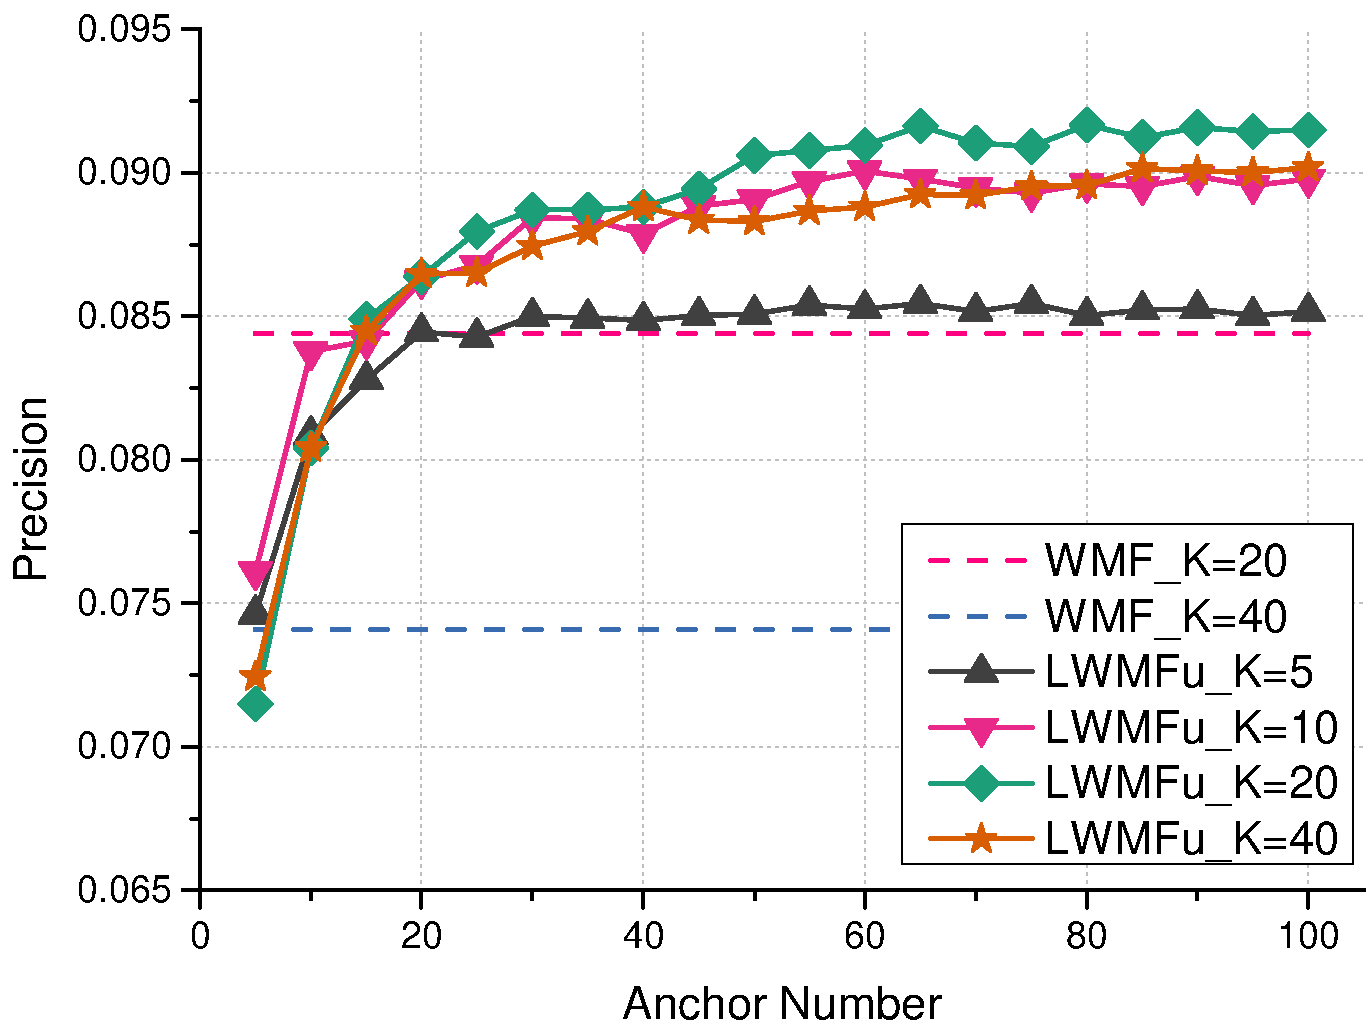
\includegraphics[width=0.486\textwidth]{Fig/lwmf/faprecision}}
	\hspace{0.0cm}
	\subfigure[Recall on Foursquare]{
		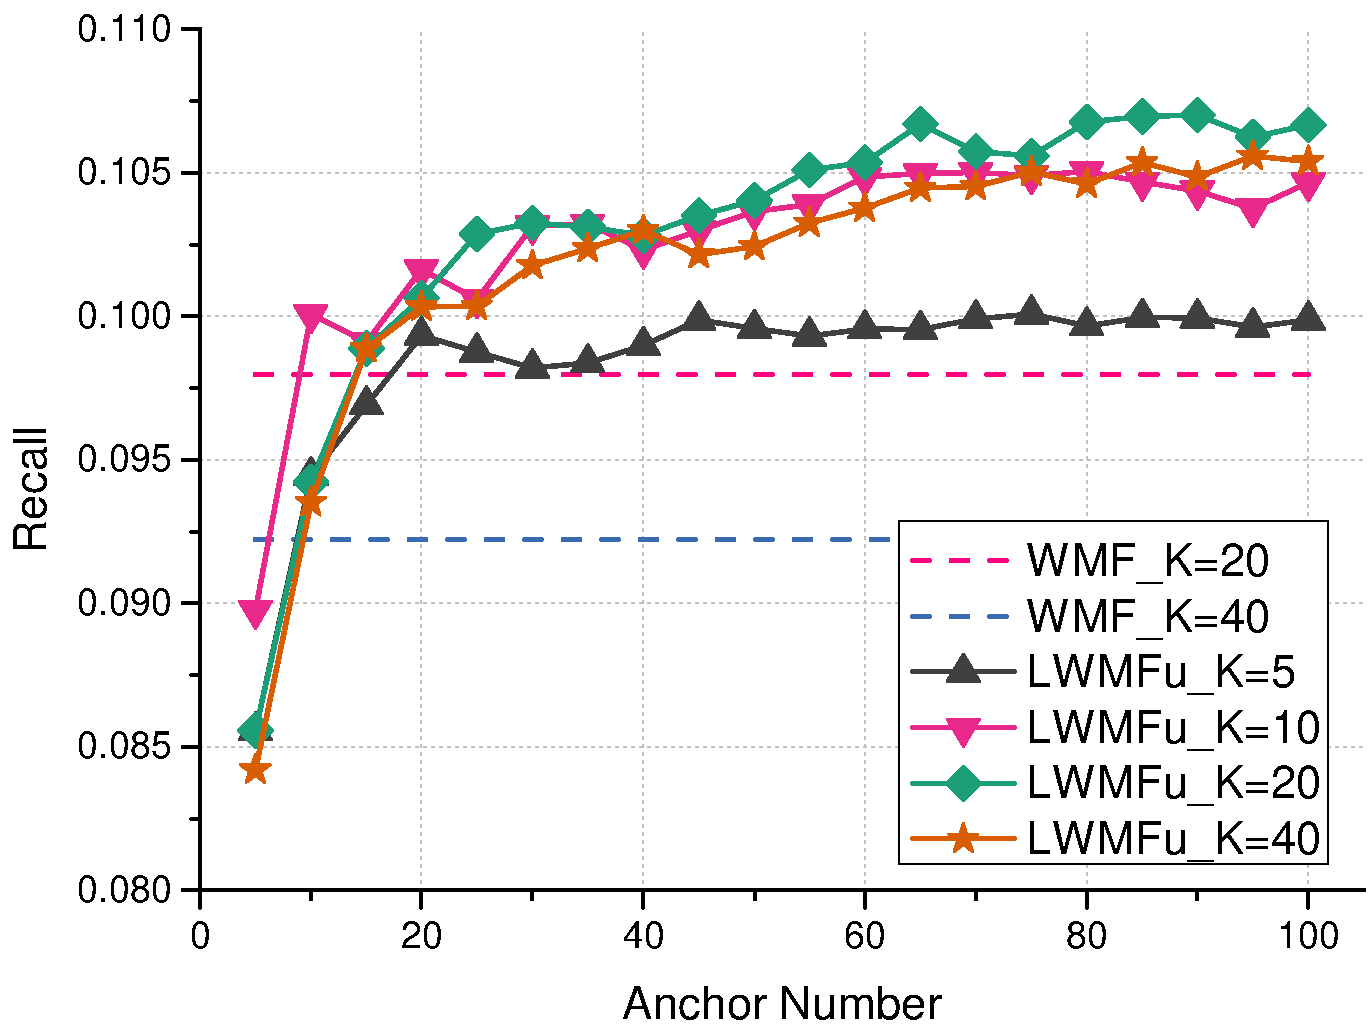
\includegraphics[width=0.486\textwidth]{Fig/lwmf/farecall}}
	\subfigure[Precsion on Gowalla]{
		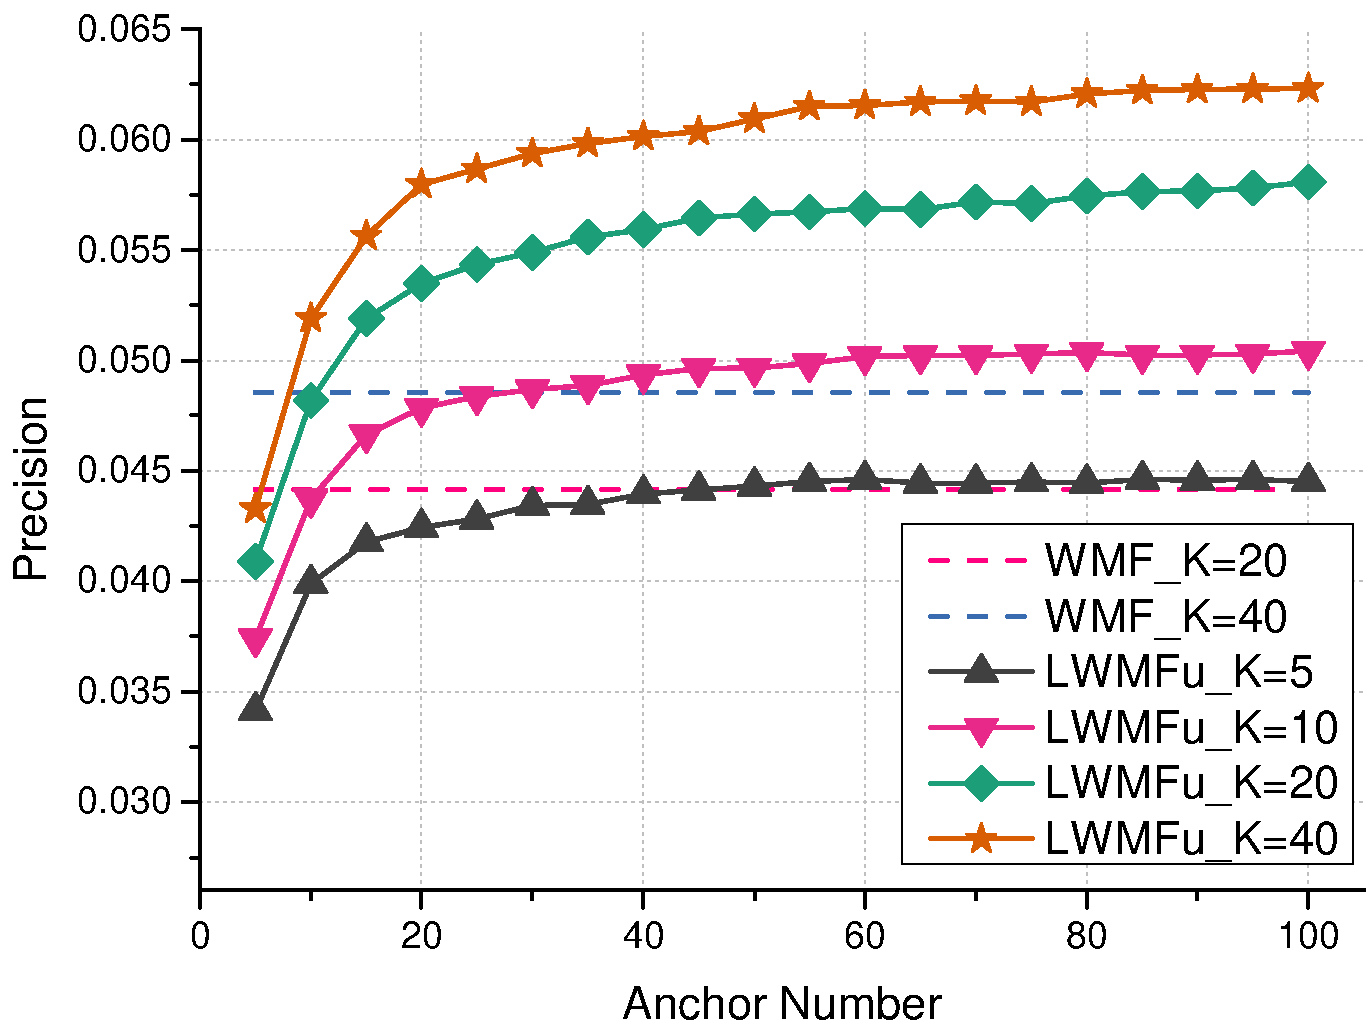
\includegraphics[width=0.486\textwidth]{Fig/lwmf/gowalla_precision}}
	\hspace{0.0cm}
	\subfigure[Recall on Gowalla]{
		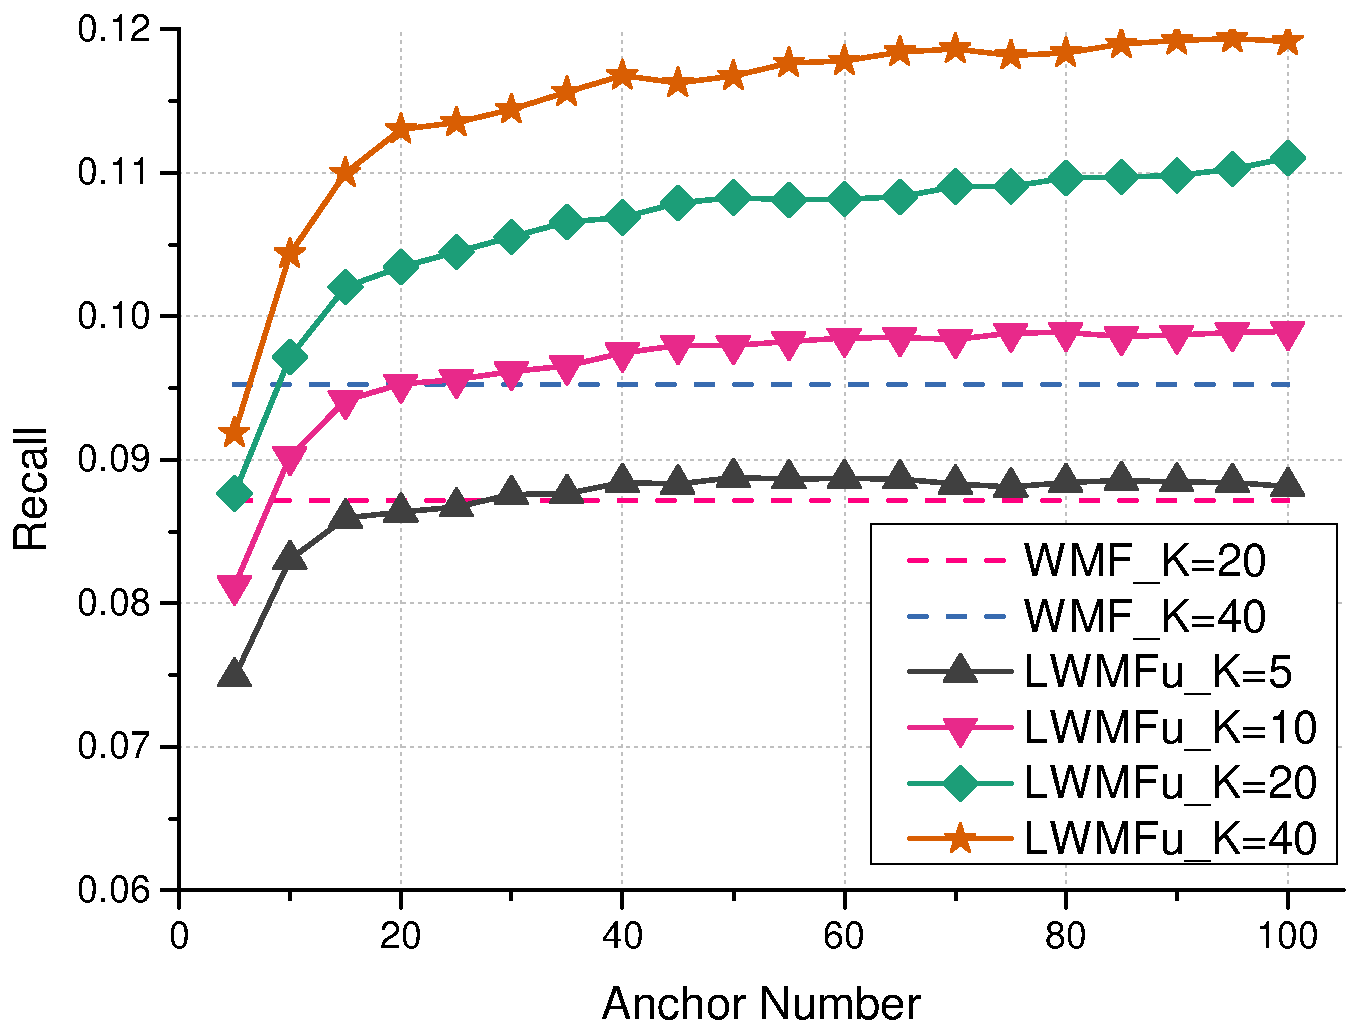
\includegraphics[width=0.486\textwidth]{Fig/lwmf/garecall}}
	
	\caption{不同锚点数量的推荐结果对比}
	\label{fig-lwmf-anchor}
\end{figure}

图~\ref{fig-lwmf-anchor}展示了不同锚点数量(即不同子矩阵个数)对本章节模型LWMF最终推荐效果的影响。在两个数据集上,LWMF的精准率和召回率都随着隐藏特征向量维度$K$提高而提高,并且LWMF在维度$K$大于等于10以后,推荐效果就优于WMF。当锚点数量$H$大于20,也就是说子矩阵数量大于20时,LWMF的推荐效果开始超过WMF,并且随着锚点数量的增多,效果越好,但同时效果边际收益却在下降。并且因为锚点的增加,子矩阵变多,训练模型的时间也会随着增加,因此用户可以根据本身时间和推荐精度需求,动态选择锚点数量。途中还可以看出当锚点数量$H$等于50的时候可以得到相对较好的实验结果。使用基于元素级最小二乘算法的WMF每一轮迭代的复杂度为$O(NK^2+MK^2+|\mathbf{R}|K)$,而整个LWMF模型每一轮迭代的复杂度为$O(\hat{H}(NK^2+MK^2+|\mathbf{R}|K))$,两者的复杂度相差$\hat{H}$倍。两个数据集中,每个子矩阵大小平均是原始矩阵的10\%左右。因此每个子矩阵的训练时间是远快于整个矩阵的分解训练。当子矩阵个数为50时,训练时间大概是WMF的5倍左右,基于推荐效果的提高,LWMF的训练时间还是能够接受的,并且LWMF经过子矩阵选择后,有着比WMF更好的数据和模型并行度,易于并行扩展。

\subsubsection{不同锚点选择方法推荐结果对比}
\begin{figure}
	\centering
	\subfigure[Precsion on Foursquare]{
		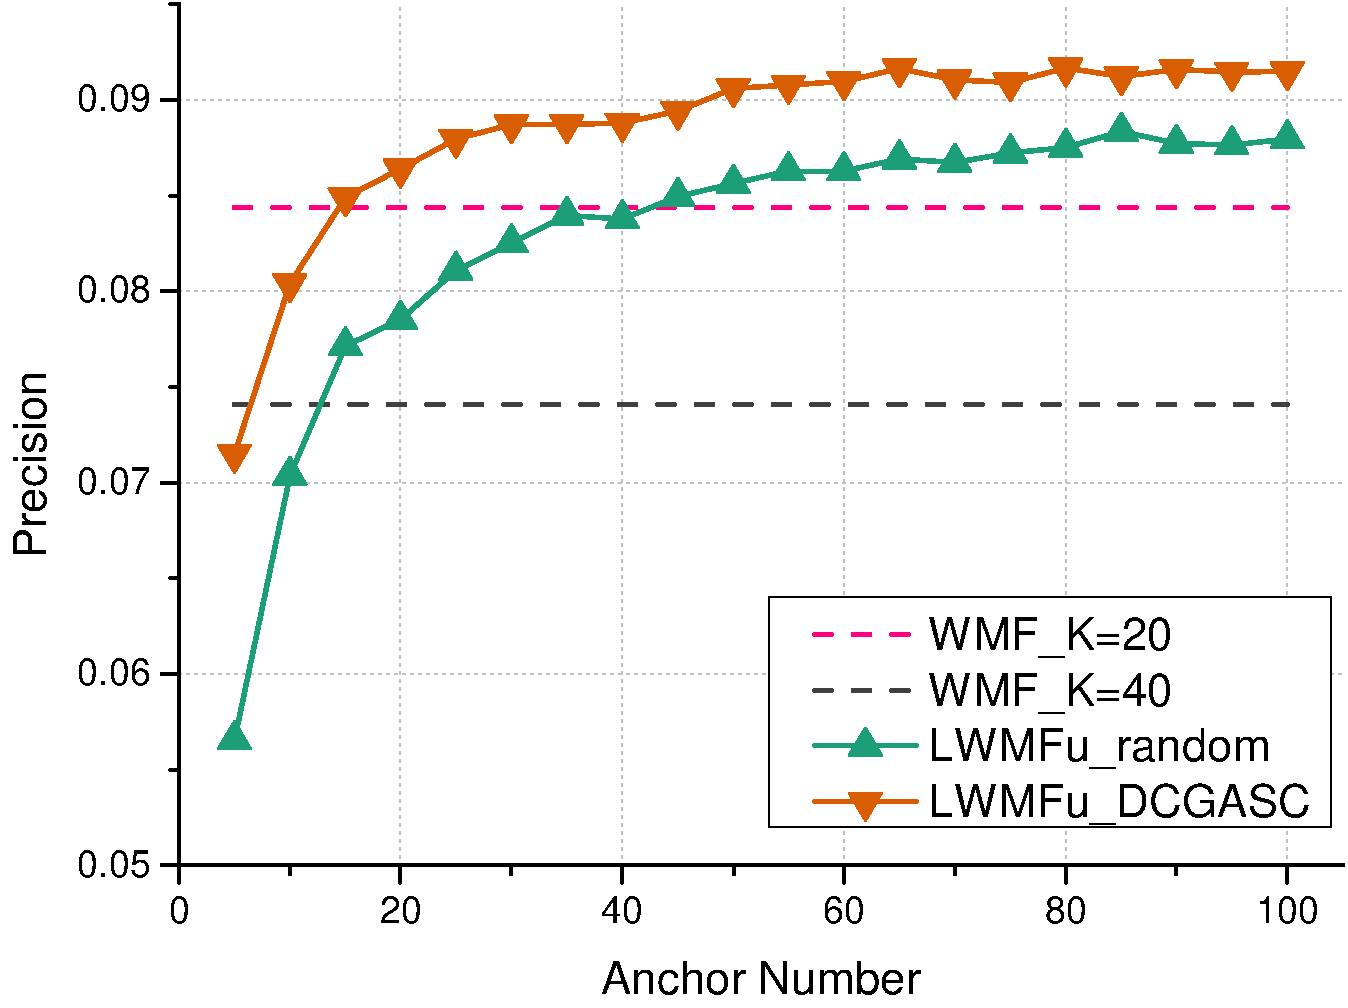
\includegraphics[width=0.486\textwidth]{Fig/lwmf/fradomprecision}}
	\hspace{0.0cm}
	\subfigure[Recall on Foursquare]{
		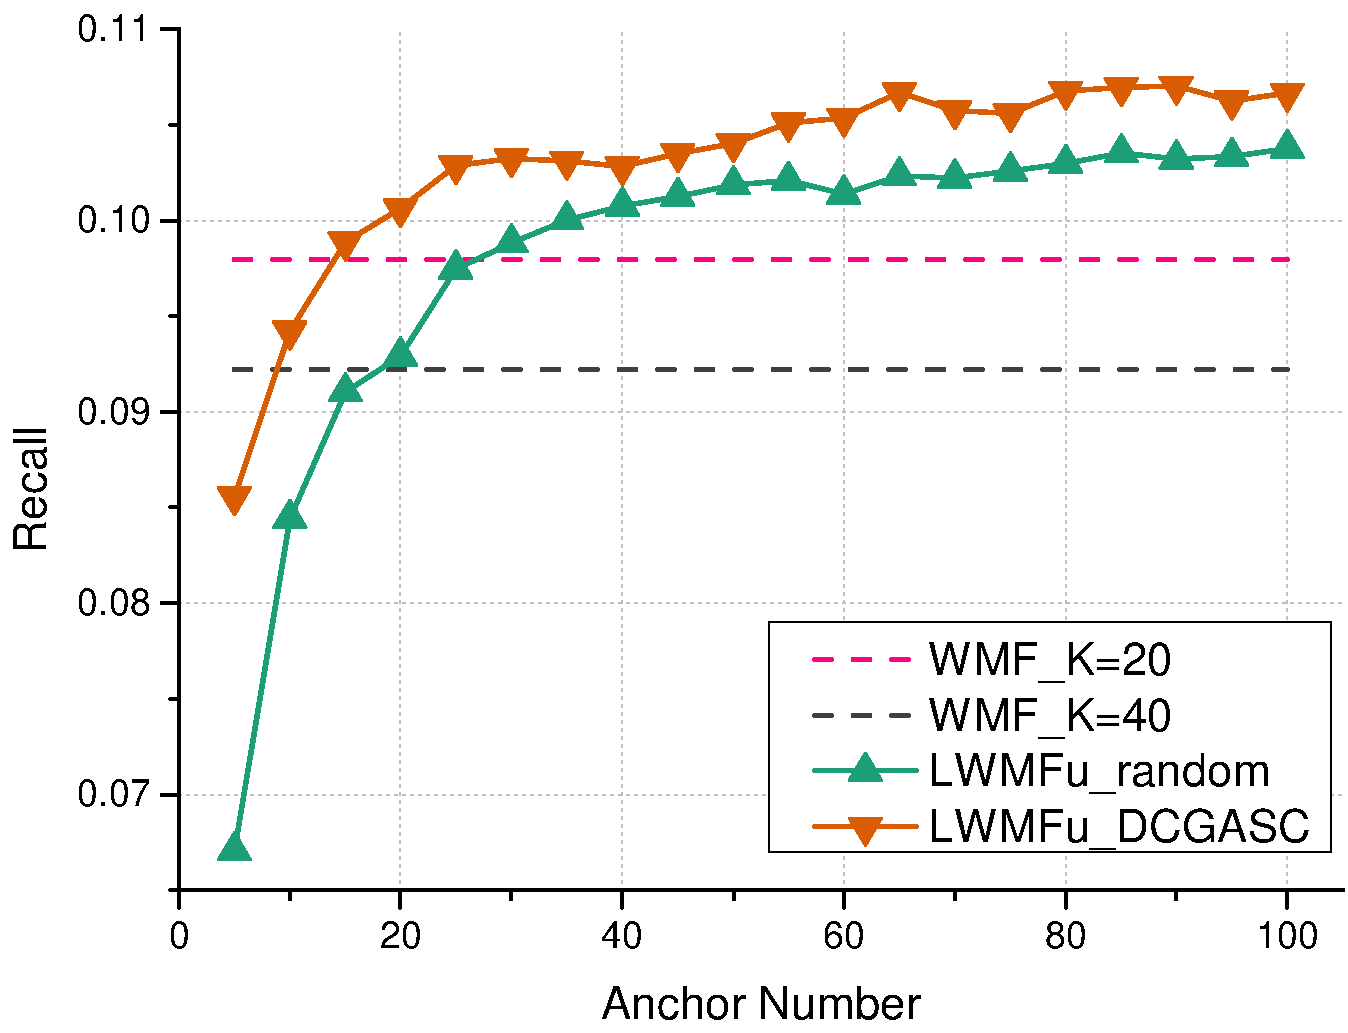
\includegraphics[width=0.486\textwidth]{Fig/lwmf/frandomrecall}}
	\subfigure[Precsion on Gowalla]{
		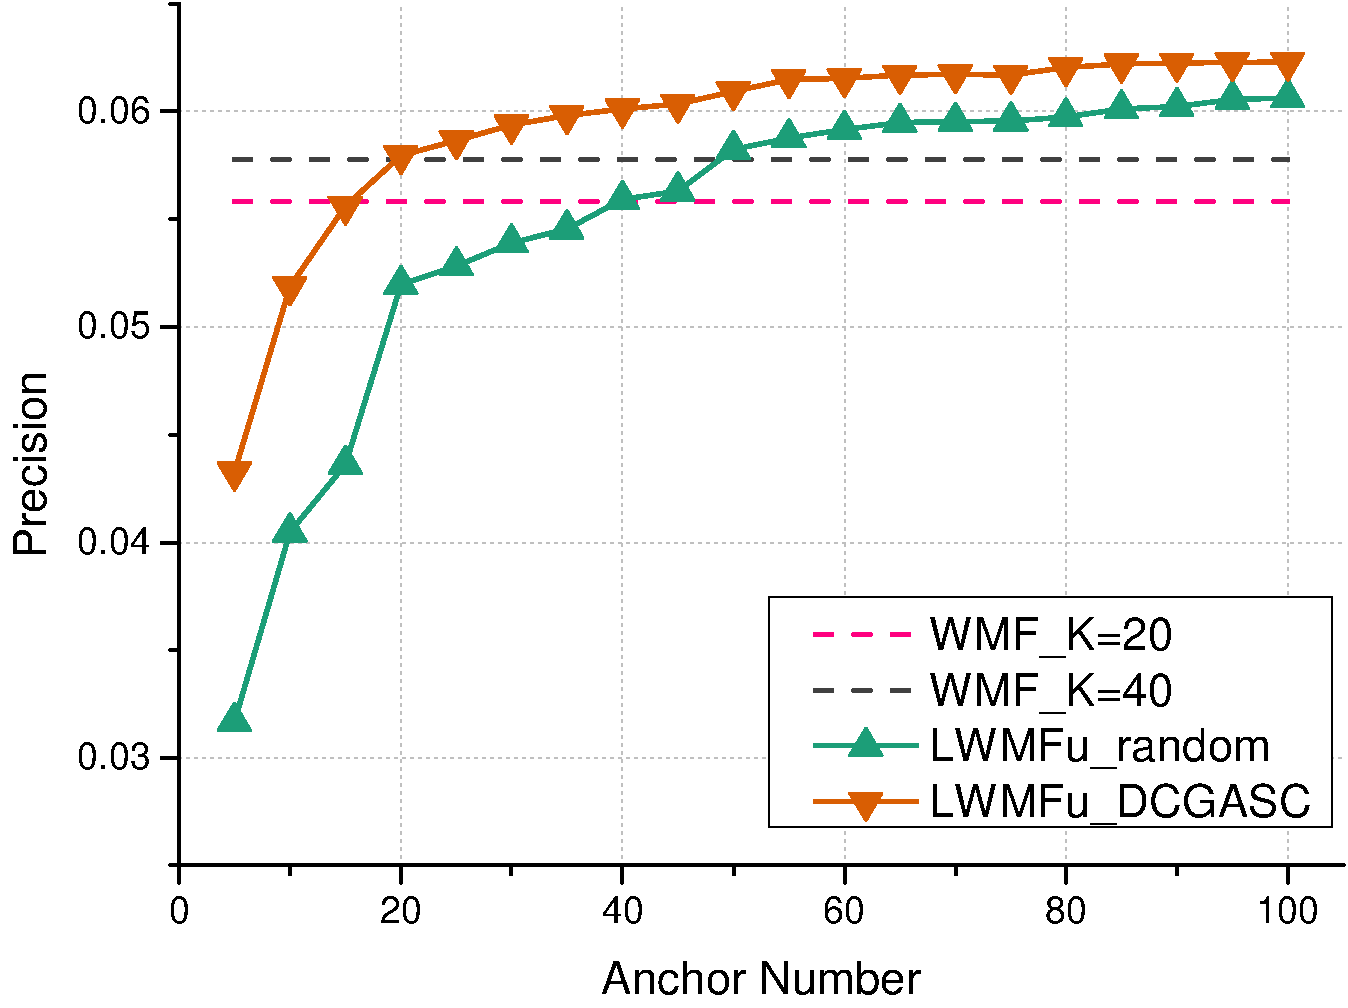
\includegraphics[width=0.486\textwidth]{Fig/lwmf/grandomprecision}}
	\hspace{0.0cm}
	\subfigure[Recall on Gowalla]{
		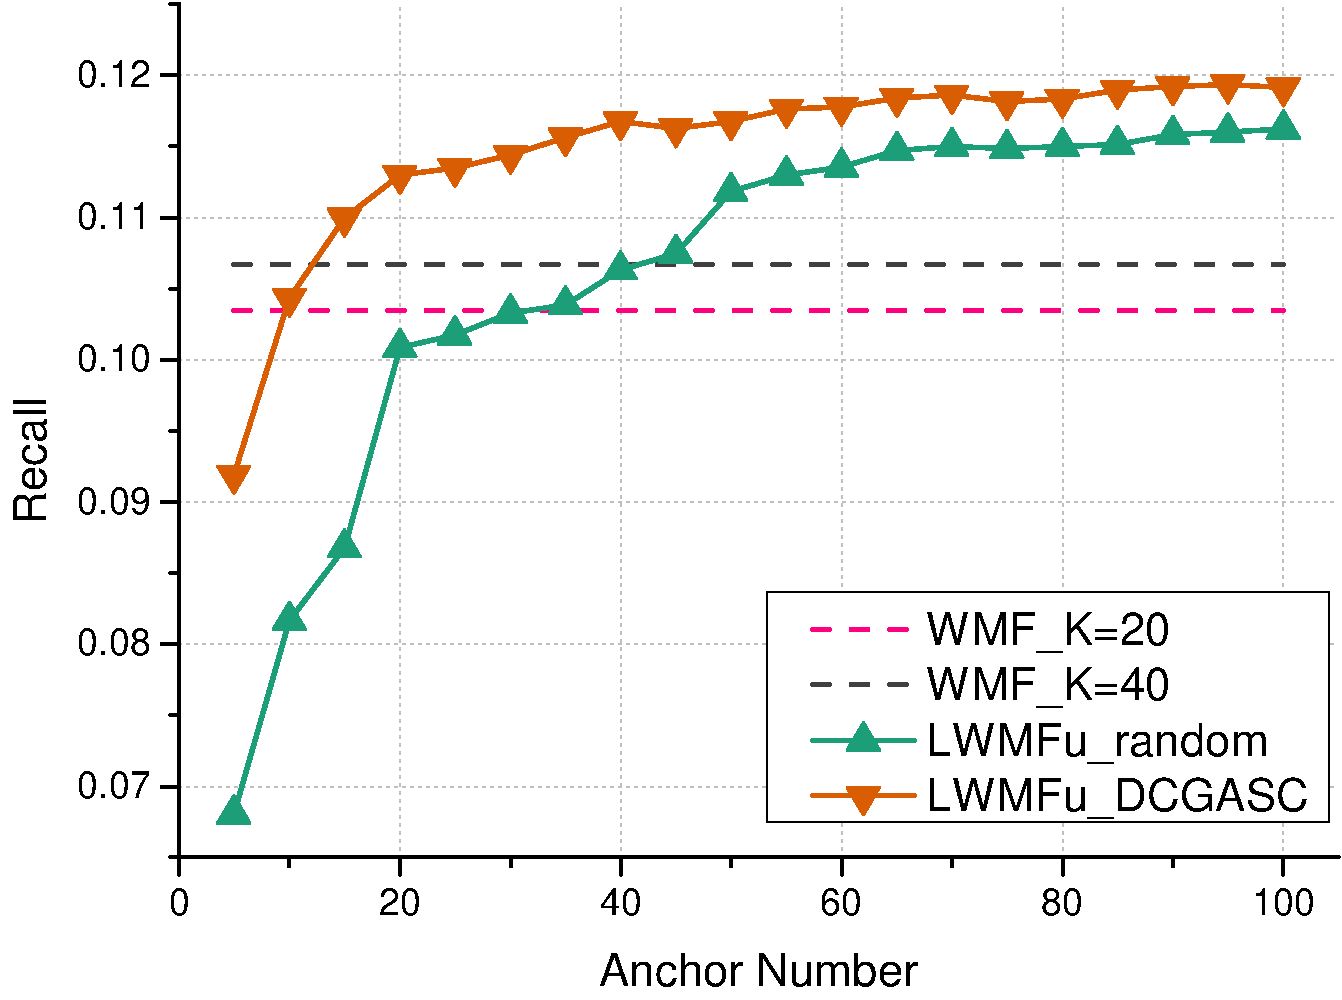
\includegraphics[width=0.486\textwidth]{Fig/lwmf/grandomrecall}}
	
	\caption{不同锚点选择方法的推荐结果对比}
	\label{fig-lwmf-random}
\end{figure}

本小节实验展示了不同锚点选择方法对本文模型LWMF最终推荐效果的影响。本实验中,DCGASC折扣系数$\alpha$设置为0.4,隐藏特征向量维度$K$在数据集Foursquare设置为20,数据集Gowalla上的维度设置为40。从图~\ref{fig-lwmf-random}中可以看出,锚点数量从0到100,基于用户选择锚点的{LWMF$_u$}的精准率和召回率都要优于基于训练集随机选择锚点的LWMF。不过随着锚点数量的增加,两者间的差距越来越小。可以肯定地是,随着锚点数量越来越多,两者性能将会差不多。极端情况下选取所有候选数据点作为锚点来选择子矩阵,{LWMF$_u$}
和{LWMF$_u$\_Random}是一样的。但考虑到锚点数量影响模型的训练时间,锚点数量越多(子矩阵越多),训练时间越久,因此从训练时间角度来看锚点数量越少越好。总体来看,{LWMF$_u$}在两个数据集上都要优于{LWMF$_u$\_Random}。

\subsubsection{不同折扣参数推荐结果对比}
\begin{figure}
	\centering
	\subfigure[Precsion on Foursquare]{
		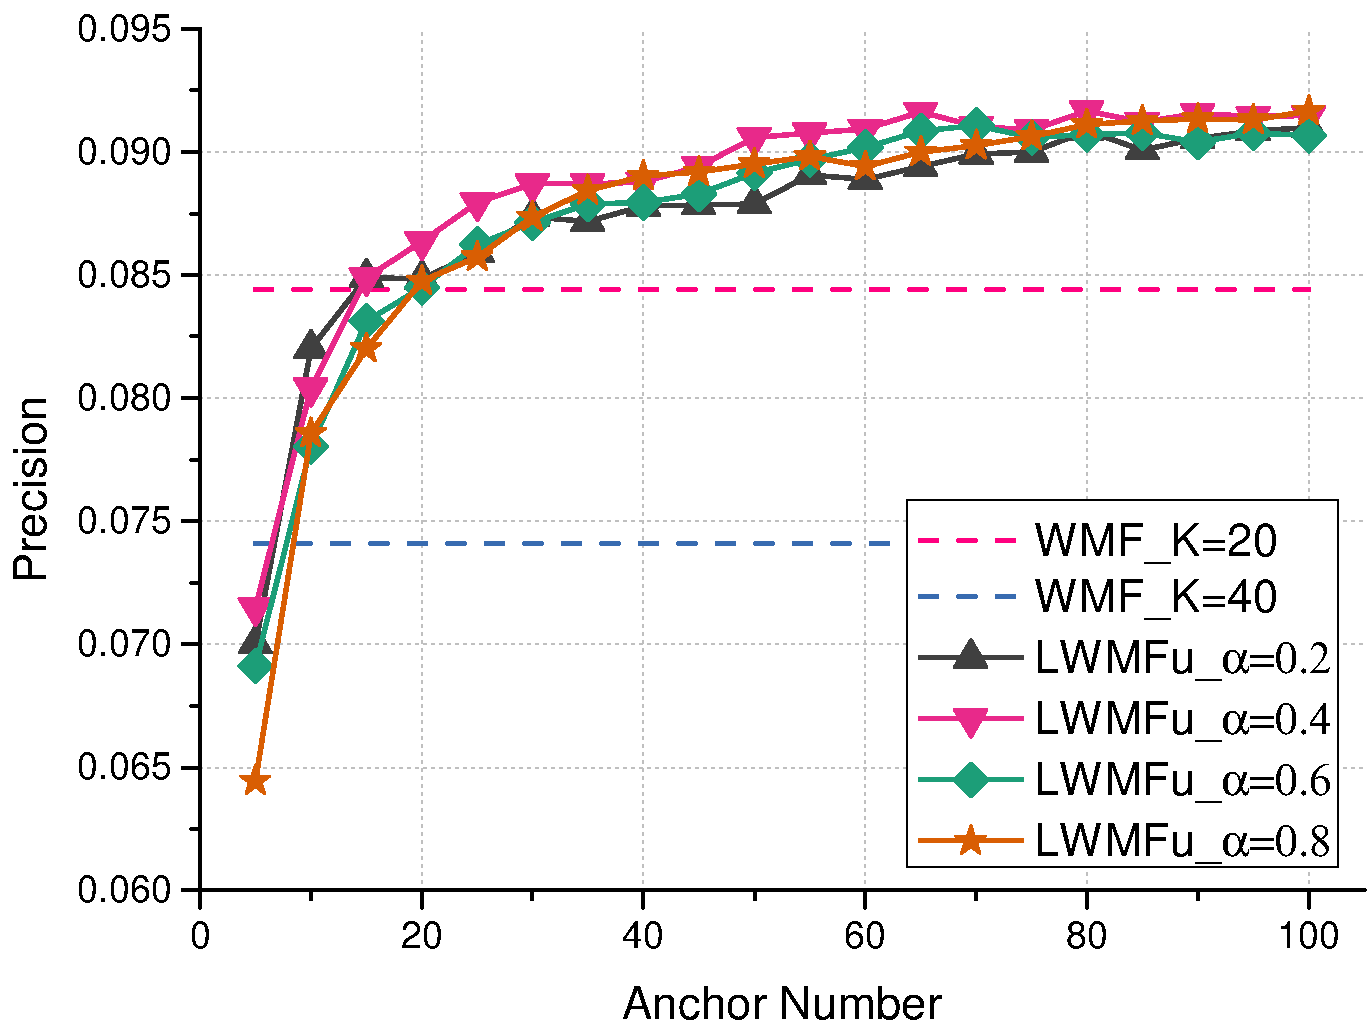
\includegraphics[width=0.486\textwidth]{Fig/lwmf/falphaprecision}}
	\hspace{0.0cm}
	\subfigure[Recall on Foursquare]{
		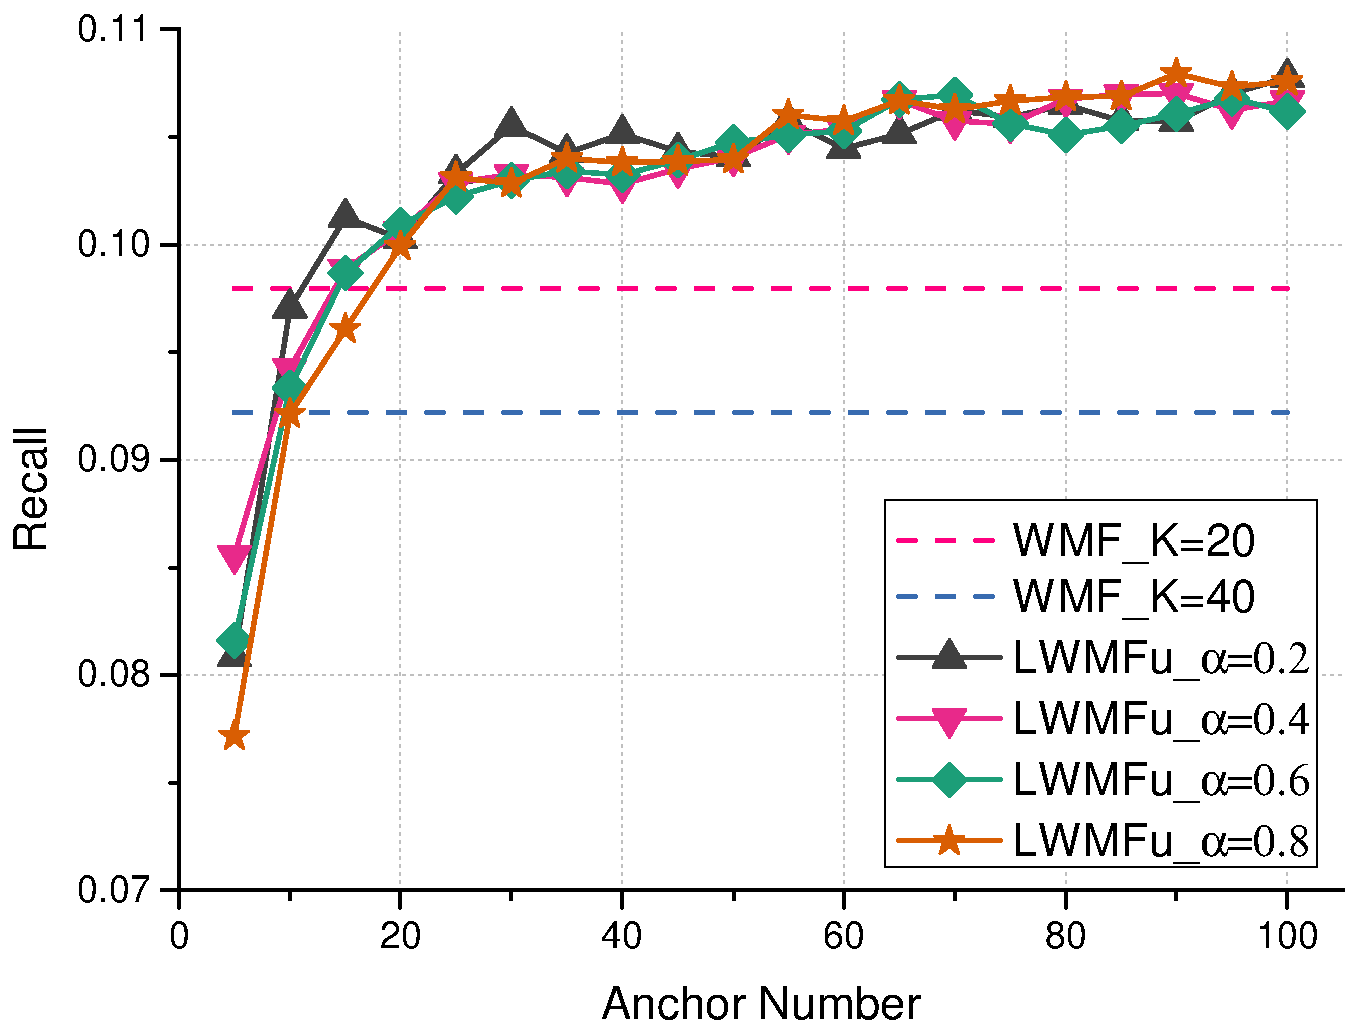
\includegraphics[width=0.486\textwidth]{Fig/lwmf/falpharecall}}
	\subfigure[Precsion on Gowalla]{
		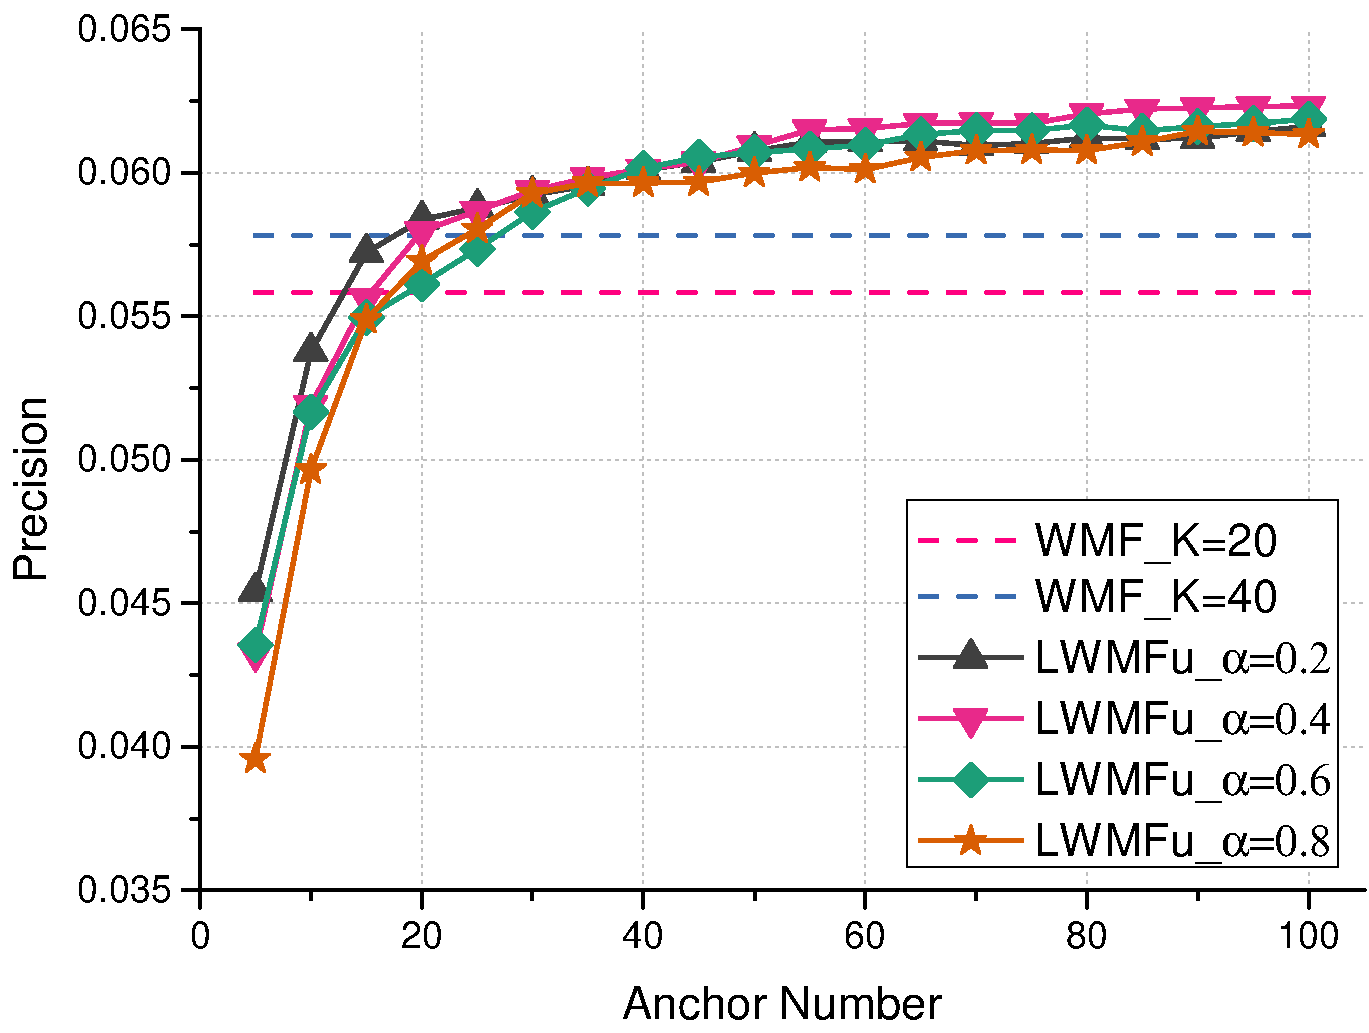
\includegraphics[width=0.486\textwidth]{Fig/lwmf/galphaprecision}}
	\hspace{0.0cm}
	\subfigure[Recall on Gowalla]{
		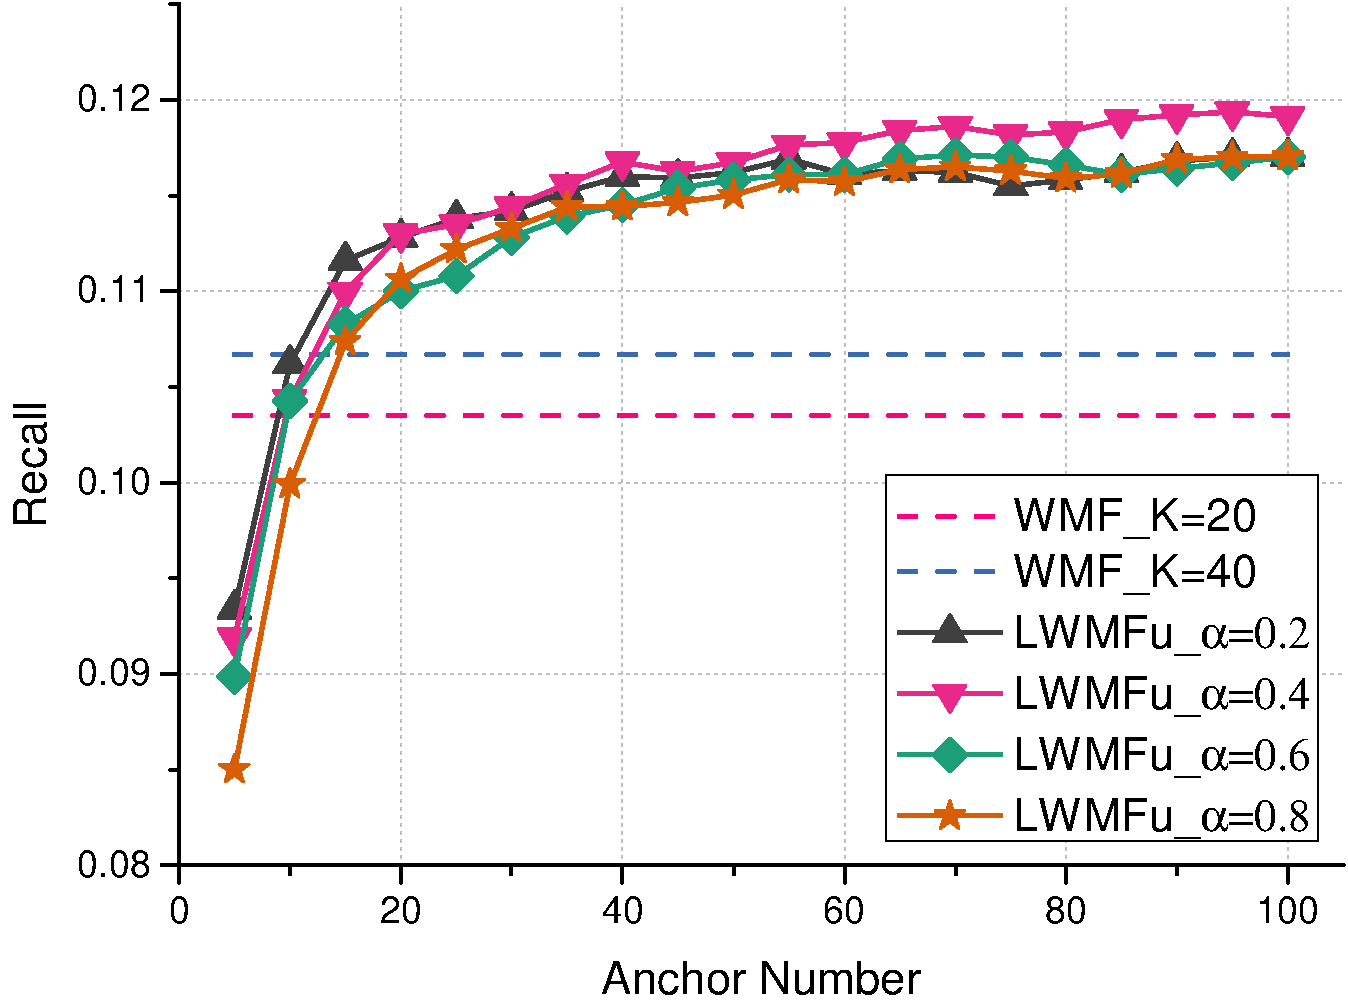
\includegraphics[width=0.486\textwidth]{Fig/lwmf/galpharecall}}
	
	\caption{不同折扣参数的推荐结果对比}
	\label{fig-lwmf-alpha}
\end{figure}

本小节研究折扣参数的不同对本文模型{LWMF$_u$}最终推荐效果的影响。跟上小节一样,隐藏特征向量维度$K$在数据集Foursquare设置为20,数据集Gowalla上设置为40。对于折扣系数$\alpha$,我们验证了范围$[0.1,0.9]$之间以0.1为间隔的推荐结果。因为不同的折扣参数,推荐的精准率和召回率较为相似,我们在本文中只画出$\alpha \in \{0.2,0.4,0.6,0.8\}$的结果曲线,如图~\ref{fig-lwmf-alpha}所示。可以看出,四个不同折扣参数之间的推荐效果差距是非常小的。相对来说,折扣参数$\alpha = 0.4$是略微优于其他参数设置。总得来说,LWMF的推荐性能对折扣参数的设置不敏感,主要依靠于锚点数量、锚点的选择方法以及隐藏特征向量维度三个方面。

\section{本章小结}
本章针对隐式反馈数据上的\textit{商品推荐}任务提出局部加权矩阵分解模型(LWMF),将整个训练数据矩阵分成一系列内部数据相似的子矩阵,然后对每个子矩阵利用加权矩阵分解得到用户和商品隐藏特征向量,最后利用隐藏向量对每个预测子矩阵进行加权平均近似原始矩阵。此外,本章工作设计了高效的子矩阵选择算法建模数据的局部信息,并改进了交替最小二乘算法进行子矩阵加权分解,刻画用户和商品的局部内在特征。同时,LWMF带来两个额外好处,缓解了数据稀疏性问题和更好地进行分布式矩阵分解。 最后,在两个真实数据集的实验表明相对于传统的WMF模型,LWMF能够有效地提高在隐式反馈数据数据上的商品推荐效果。

\clearpage
\phantom{s}
\clearpage
\chapter{基于多主题矩阵分解的评分预测}
\label{chapter-bpmtmf}
本章重点介绍针对显式评分数据进行\textit{评分预测}的研究内容。首先,章节~\ref{sec-bpmtmf-intro}描述本章的研究内容和大概的解决思路。接着,章节~\ref{sec-bpmtmf-model}具体介绍本章提出的评分预测模型及其优化算法,并描述了模型与现有的局部矩阵分解模型之间的联系。随后在章节~\ref{sec-bpmtmf-experiments}中分析基于两个电影评分数据集上的实验结果。最后总结本章工作研究内容。

\section{引言}
\label{sec-bpmtmf-intro}


上一章介绍了个性化推荐系统的一个典型任务\textit{商品推荐},即根据用户的历史行为信息推荐用户感兴趣的商品。本章节介绍个性化推荐系统的另一个典型任务\textit{评分预测},是基于用户历史的显式评分数据预测用户对给定商品的评分,用以表达用户对商品的满意程度。第~\ref{chapter:relatedwork}章中介绍了大量的\textit{评分预测}模型,其中章节~\ref{sec-related-pmf}详细介绍了一个针对\textit{评分预测}的经典模型,概率矩阵分解模型(PMF)~\cite{salakhutdinov2007probabilistic}。该模型在许多真实竞赛中拥有良好的表现,例如Netflix百万美元竞赛得主的模型中的一个主要模型就是矩阵分解。PMF利用零均值球面高斯分布作为隐藏特征的先验分布,使用高斯分布对评分信息建模,将用户和商品属性投射到低秩空间中,然后使用用户和商品隐藏特征向量的点积还原评分矩阵的缺失值。近期,针对\textit{评分预测}任务的局部矩阵分解模型~\cite{lee2013local}已被验证比传统的矩阵分解模型更加有效。它的主要思想是将原始评分矩阵分成几个较小的子矩阵,然后利用局部结构来获得更好的低秩近似。然后在每个子矩阵中,应用标准矩阵分解技术来为用户和商品生成子矩阵特定的隐藏特征向量。通常,使用聚类技术获得这些子矩阵。通过组合多个子矩阵$\mathbf{\mathbf{R}^1,\mathbf{R}^2,..., \mathbf{R}^H}$以及对应的权重$\{\mathbf{V}^1,\mathbf{V}^2,...,\mathbf{V}^H\}$重新构成原始矩阵$\mathbf{R}$:

\begin{equation}
\label{eq-bpmtmf-localmf}
\hat{\mathbf{R}}_{um}= \frac{1}{\mathbf{Z}_{um}}\sum_{h=1}^H \mathbf{V}_{um}^{h}\mathbf{R}_{um}^{h}
\end{equation}
其中$\mathbf{Z}_{um}=\sum_{h=1}^H\mathbf{V}_{um}^h$是归一化因子,$\mathbf{V}_{um}^h$代表了项$\mathbf{R}_{um}^h$在子矩阵$\mathbf{R}^h$中的权重。在第\ref{chapter-lwmf}章已经说明这类矩阵集成的方法主要有两个关键问题:1)如何产生子矩阵和(2)如何设置子矩阵的集合权重。当前已经有一些工作去解决这两点,例如使用随机抽样~\cite{MJT11},使用锚点扩展最近邻数据点~\cite{lee2013local,lee2014local},或者基于联合硬聚类分割的方法~\cite{chen2015wemarec}。

虽然这些研究在某种程度上比传统矩阵分解模型有所改进,但缺乏一种更可信的方法来表示局部矩阵分解。通过回顾以前的研究~\cite{MJT11,lee2013local,lee2014local,chen2015wemarec},有两个重要的发现:(1)每个子矩阵可以被认为是用户和商品的局部聚类; (2)用户或商品在不同子矩阵中具有多个隐藏特征表示。受这两个观察的启发,本章提出一种新颖的贝叶斯概率多主题矩阵因子分解模型(Bayesian Probabilistic Multi- Topic Matrix Factorization ,简称BPMTMF)来进行\textit{评分预测}。本章的模型包括两个部分,即对用户访问商品行为建模和对评分建模。对于第一部分,本章将用户访问过的商品视为一个文档,并且利用主题模型中主题来``聚类''商品,每个主题是关于商品的多项式分布。随后,用户具有在主题集合上的多项式分布(即主题分布)。基于这样的主题,本章进一步为用户和商品设置主题特定的隐藏特征向量。本章工作将以一个完整的贝叶斯方法整合上述两个部分。本章提出模型的最终评分预测是由各个主题特定的隐藏特征向量生成的评分组合而成。本章节模型使用贝叶斯概率的方法描述了公式~\ref{eq-bpmtmf-localmf}的思想,即每个主题被认为是一个聚类。使用多主题隐藏特征表示,本章模型能更好地反映用户和商品在\textit{评分预测}中的复杂特性。使用主题模型的另一个重要优点是BPMTMF具有更好的模型可解释性。由于主题模型能够有效地发现共现的主题语义~\cite{blei2003latent},BPMTMF中产生的相同主题的商品也是高度相关的。使用此类方法,一个主题得到的商品也比以前的研究~\cite{MJT11,lee2013local,lee2014local,chen2015wemarec}中获得的更加一致。将主题作为上下文信息,本章工作可以分析用户的评分喜好在不同的主题中是如何变化的。

值得注意的是,在现有研究工作中研究人员已经做了一些将主题模型与矩阵分解模型结合的尝试,包括CTM~\cite{wang2011collaborative},HFT~\cite{mcauley2013hidden}和ETF~\cite{zhang2014explicit}。然而,这些方法主要是将评分结合到文本信息的主题模型中,并且期望结合两种模型的优点。通常,这类模型使用单个全局的矩阵分解模型建模评分数据,因此其不适合于局部矩阵分解模型。因此本章工作是针对显式评分数据第一次提出了一种局部矩阵分解的贝叶斯模型,它将主题模型与概率矩阵分解模型结合起来。通过使用主题作为聚类依据使得模型有更好的可解释性。在大型真实世界数据集的实验表明了所提出的模型与多个竞争性基线模型相比具有更高的评分预测有效性。

% \section{相关工作}
% 在本节中,我们将回顾相关工作。

% 矩阵因式分解。 MF [Paterek,2007; Mnih和Salakhutdinov,2007; Koren等人,2009]是一种重要的基于模型的协同过滤方法。 MF通过将用户和项目投影到潜在的低维空间中来构造低秩近似。 此外,已经通过使用高斯分布来建模具有零均值球面高斯先验的观察到的评级的概率矩阵因子分解(PMF)。 实质上,PMF可以被认为是规则化奇异值分解的概率实现。 此外,Salakhutdinov和Mnih [Salakhutdinov和Mnih,2008]提出了一个完整的贝叶斯公式PMF。 由于MF,双向MF和SVD ++的扩展已经在[Koren等人,2009]中提出。 偏置MF包括用户偏好和项目偏差,而SVD ++使用隐式反馈来改善用户偏好建模。

% 最近,几个关于使用子矩阵集合进行更好低阶近似的研究,包括DFC [Mackey et al。,2011],LLORMA [Lee et al。,2013; 2014],ACCAMS [Beutel等,2015]和WEMAREC [Chen等,2015]。这些方法将原始矩阵分割成若干较小的子矩阵,并且将单独的局部MF应用于每个子矩阵。使用多个局部MF的集合获得最终预测。通常,使用启发式适配的基于聚类的技术用于子矩阵生成。我们简要回顾这些研究。 Mackey et al。 [Mackey et al。,2011]引入了一个除法因子组合(DFC)框架,其中矩阵分解的昂贵任务被随机分为较小的子问题。 LLORMA [Lee et al。,2013; 2014]使用非参数核平滑方法搜索最近邻; WEMAREC [Chen et al。,2015]采用Bregman共聚类[Dhillon et al。,2003]技术分割原始矩阵; ACCAMS采用加法共聚类方法[Shan and Baner-jee,2008]来推导子矩阵并使用高斯分布来预测等级。我们的工作是建立在上述研究基础上的,然而,我们建议使用概率主题模型来创建“软”聚类,通过将主题模型与概率MF相结合,进一步开发一个完整的贝叶斯模型。

% 与主题模型的矩阵因式分解。在文献中,研究人员已经做了几项将主题模型与MF结合的尝试,包括CTM [Wang and Blei,2011],HFT [McAuley和Leskovec,2013]和ETF [Zhang et al。,2014]。然而,这些方法主要旨在将评级结合到主题模型中,并且集中于组合来自两种模型的优点。通常,使用单个MF分量,其不适合于本地MF。


% \subsection{概率潜在语义分析}\label{sec:plsa}
% 概率潜在语义分析(PLSA)\cite{Hofmann1999}是一种主题模型(topic  model)。主题模型是对文字隐含主题进行建模的方法。它克服了传统信息检索中文档相似度计算方法的缺点,并且能够在海量互联网数据中自动寻找出文字间的语义主题。和基于奇异值分解的隐语义分析不同,PLSA是一个生成模型,因此基于统计学的推论方法,最大似然方法\cite{Moon1996} 均可以用来学习模型参数。
% \begin{figure*}[htbp]
% 	\centering
% 	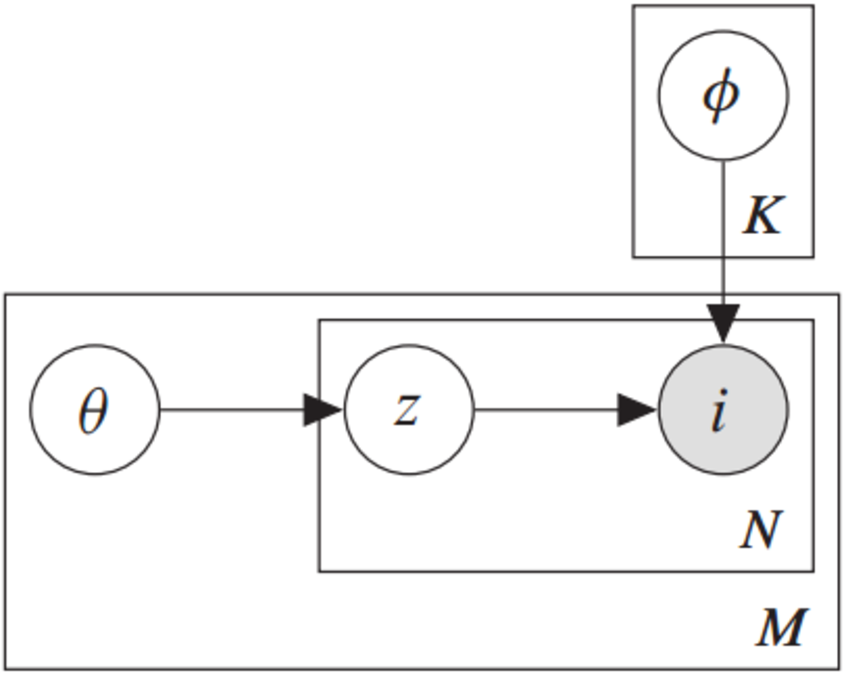
\includegraphics[width=0.4\textwidth]{Fig/bpmtmf/plsa}	
% 	\caption{概率隐藏语义分析}
% 	\label{fig-bpmtmf-plsa}
% \end{figure*}

% 图\ref{plsa}是PLSA的图模型表示。M表示用户个数,N表示POI 的个数。$\theta$是每个用户的主题的先验分布。给定一个用户u,多项式分布$\theta_u$表示该用户各个主题的分布。多项式分布$\phi_k$ 表示主题k中POI的分布。生成过程如下:
% \begin{itemize}
% 	\item 对每个用户u:
% 	\begin{itemize}
% 		\item 对$n_u$个POI采样
% 		\item 对每个$s \in {i,...,n_u}$
% 		\begin{itemize}
% 			\item z~DISC($\Theta_u$)
% 			\item 选择一个POI p~DISC($\Phi_z$)
% 		\end{itemize}
% 	\end{itemize}
% \end{itemize}

% 概率公式如公式\ref{equ:pgm2},\ref{equ:pgm3}:
% \begin{equation}
% P(d_i,w_j)=P(d_i)P(w_j|d_i)
% \label{equ:pgm2}
% \end{equation}
% \begin{equation}
% P(w_j|d_i)=\sum_{k=1}^{K}P(w_j|z_k)P(z_k|d_i)
% \label{equ:pgm3}
% \end{equation}

% PLSA的EM求解如下:

% E步如公式\ref{equ:pgm4}:
% \begin{equation}
% \gamma(z_ijk)=p(z_k|d_i,w_j)=\frac{p(d_i)p(z_k|d_i)p(w_j|z_k)}{\sum_{k=1}^{K}p(z_k|d_i)p(w_j|z_k)}=\frac{p(z_k|d_i)p(w_j|z_k)}{\sum_{k=1}^{K}p(z_k|d_i)p(w_j|z_k)}
% \label{equ:pgm4}
% \end{equation}

% M步如公式\ref{equ:pgm5},\ref{equ:pgm6}:
% \begin{equation}
% p(w_j|z_k)=\frac{\sum_{i=1}^{N}n(d_i,w_j)P(z_k|d_i,w_j)}{\sum_{m=1}^{M}\sum_{i=1}^{N}n(d_i,w_m)P(z_k|d_i,w_m)}
% \label{equ:pgm5}
% \end{equation}
% \begin{equation}
% p(z_k|d_i)=\frac{\sum_{j=1}^{M}n(d_i,w_j)P(z_k|d_i,w_j)}{n(d_i)}
% \label{equ:pgm6}
% \end{equation}

% 卡尔加里大学的一篇论文中\cite{Zhou2012}将基于内存的两种推荐方法(基于用户的和基于内存的)以及PLSA 进行对比,实验评估精度和召回两个指标,实验结果表明PLSA一直表现好于两周基于内存的推荐方法。

% 与基于内存的推荐算法相比,PLSA不依赖于相似度计算,用一种概率的方式解释了用户对POI 的签到行为。
% \subsection{隐含狄利克雷分布}
% 上一节提到的PLSA方法依赖于最大似然估计且没有对似然$\theta$做假设,所有的θ是等概率的,因此最优的参数集是由观察到的数据确定的。PLSA主要的缺点是参数的数量和数据集的大小成比例,并且没有合适的方法处理不可见的数据点。因此,贝叶斯学派提出隐含狄利克雷分布(Latent Dirichlet Allocation,LDA)\cite{Blei2003}。

% PLSA中Φ和θ是模型的参数,对应多项式分布,根据:

% Dirichlet先验+多项式分布的数据→后验分布为Dirichlet分布

% 所以在LDA中,为$\phi$和$\theta$增加Dirichlet先验分布。
% \begin{figure*}[htbp]
% 	\centering
% 	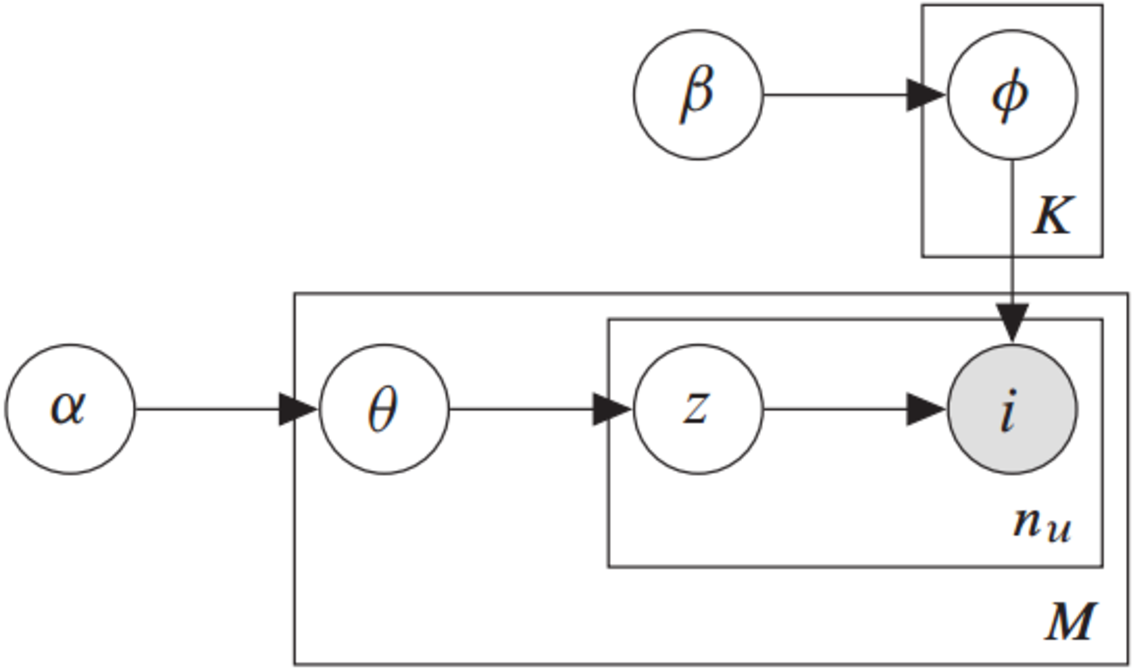
\includegraphics[width=0.4\textwidth]{Fig/bpmtmf/lda}	
% 	\caption{潜在狄利克雷分布}
% 	\label{fig-bpmtmf-lda}
% \end{figure*}
% 如图\ref{lda}所示,这个概率图可以分解为两个主要的物理过程:

% 1. $\alpha  \to \theta  \to z$ ,这个过程表示某一用户u的签到POI,首先由$\alpha$生成$\theta$,然后由$\theta$决定用户u第i个签到的POI的主题。

% 2. $\beta \to \phi \to i |k=z_{u,i}$ ,这个过程表示用如下方法生成用户u 第i个签到的POI:在$\Phi_1…\Phi_k$ 中,挑选$k=z_{u,i}$的,根据概率生成POI i。

% 联合分布如公式\ref{equ:pgm7}:
% \begin{equation}
% p(\vec{w},\vec{z}|\vec{\alpha},\vec{\beta})=p(\vec{w}|\vec{z},\vec{\beta})p(\vec{z}|\vec{\alpha})=\prod_{k=1}^{K}\frac{\Delta(\vec{n_k}+\vec{\beta})}{\Delta(\beta)}\prod_{m=1}^{M}\frac{\Delta(\vec{n_m}+\vec{\alpha})}{\Delta(\alpha)}
% \label{equ:pgm7}
% \end{equation}

% \section{多主题矩阵分解}

% \subsection{模型概览}
% n this paper, we assume that each user (or item) has different topic preference  and has a latent vector $\mathcal{P}_u^{h}\in \mathbb{R}^K$ (or $\mathcal{Q}_m^{h}\in \mathbb{R}^K$) for each topic $k$ instead of only one latent vector globally. As Figure \ref{fig:mamf} shows, we first divide data matrix into several submatrices.  Users (or items) in the same su-matrix are similar while users (or items) in the different submatrix do not have similar behavior. Then \textit{PBMF} is applied in each submatrix to get latent feature vectors for each topic. We propose a method called \textit{MTMF} under this idea. \textit{MTMF} combines traditional matrix factorization methods with topic modeling. Topic modeling specifies a co-occurrence data model which associates a latent factor with each single observation user-item pair $\langle u,i\rangle$. The generative process of \textit{MTMF} is as follows,
% \begin{itemize}
% 	\item[1.] For each user $u \in U$
% 	\begin{itemize}
% 		\item[(a)] Draw the number $n_u$ of item selections;
% 		\item[(b)] For each of the $n_u$ items to be generated;
% 		\begin{itemize}
% 			\item[i.] Draw a user topic $z_k\sim Disc(\theta_u)$
% 			\item[ii.] Draw the user latent factor $\mathcal{P}^{h}_u\sim \mathcal{N}(\mathcal{P}_u^{h}|0,\sigma_{\mathcal{P}^{h}}^2\mathbf{I})$ of topic $k$;
% 			\item[iii.] Draw an item $m\sim Disc(\phi_{z_k})$
% 			\item[iv.] Draw the item latent factor $\mathcal{Q}^{h}_m\sim \mathcal{N}(\mathcal{Q}_m^{h}|0,\sigma_{\mathcal{Q}^{h}}^2\mathbf{I})$ of topic $k$;
% 			\item[v.] Draw the rating $R_{um}\sim \mathcal{N}(\mathbf{R}_{um}|{\mathcal{P}_u^{h}}^\intercal\mathcal{Q}_m^{h},\sigma^2)$
% 		\end{itemize}
% 	\end{itemize}
% \end{itemize}
% So for user $u$ (or item), there are $K$ topic distribution value and $K$ latent feature vectors to model. Note that the topic model part can be replaced or extended by different probabilistic graphical models.

% The data likelihood function $P(\mathbf{R}|\Theta)$ for user-item matrix can be expressed as
% \begin{align}
% % \nonumber to remove numbering (before each equation)
% P(\mathbf{R}|\Theta)=&\prod_{\langle u,m\rangle}\sum_k^K\theta_{u,k}\phi_{k,m} \mathcal{N}(\mathbf{R}_{um}|{\mathcal{P}_u^{h}}^\intercal\mathcal{Q}_m^{h},\sigma^2)\nonumber \\
% & \mathcal{N}(\mathcal{P}_u^{h}|0,\sigma_{\mathcal{P}^{h}}^2\mathbf{I})\mathcal{N}(\mathcal{Q}_m^{h}|0,\sigma_{\mathcal{Q}^{h}}^2\mathbf{I}) \nonumber \\
% & \mathcal{N}(\mathbf{a}_u|0,\sigma^2_{\mathbf{a}}) \mathcal{N}(\mathbf{b}_m|0,\sigma^2_{\mathbf{b}})
% \end{align}
% where $\sum_{k}\theta_{u,k} = 1$ and $\sum_{m}\phi_{k,m} = 1$.

% In general, each prediction is estimated by the weighted sum of the topic ratings,
% \begin{align}
% \hat{R}_{um} = \frac{\sum_{k=1}^K\theta_{u,k}\phi_{k,m}({\mathcal{P}_u^{h}}^\intercal\mathcal{Q}_m^{h}+\mathbf{A}_u^{h}+\mathbf{B}_m^{h}+\mu)}{\sum_{k=1}^K\theta_{u,k}\phi_{k,m}}
% \end{align}
% We use global mean of observations in the training set as the predicted rating when $\sum_k^K\theta_{u,k}\phi_{k,m}=0$.

% \subsection{参数估计}
% \label{subsec:alg}
% We develop an Expectation Maximization algorithm  to learn the topics and latent feature vectors. By applying the EM framework, the complete data expectation log-likelihood of $\mathbf{R}$ given four regularization factors can be expressed as:
% \begin{align}
% &\mathbb{Q}(\Theta,\Theta') = \sum_{\langle u,m\rangle}\sum_k \gamma_{u,m,k}(\Theta')\{\log \theta_{k,u}+\log \phi_{m,k}-\nonumber \\
% & (\mathbf{R}_{um}-{\mathcal{P}_{u}^{h}}^\intercal\mathcal{Q}_{m}^{h}-\mathbf{A}_{u}^{h}-\mathbf{B}_{m}^{h}-\mu)^2
% -\lambda_{\mathcal{P}}{\mathcal{P}_{u}^{h}}^\intercal\mathcal{P}_{u}^{h} \nonumber \\
% &-\lambda_{\mathcal{Q}}{\mathcal{Q}_{m}^{h}}^\intercal\mathcal{Q}_{m}^{h}-\lambda_{\mathbf{A}}{\mathbf{A}_{u}^{h}}^2 -\lambda_{\mathbf{B}}{\mathbf{B}_{m}^{h}}^2 \}
% \end{align}

% We first use the \textit{PBMF} to initialize multi-topic user factors $\mathcal{P}$ and multi-topic item factors $\mathcal{Q}$. At first, we get topic distribution $\theta_u$ for user $u$ and  item distribution $\phi_k$ for topic $k$ by Equations (\ref{equ:gamma}), (\ref{equ:theta}) and (\ref{equ:phi}) while multi-topics latent factors are fixed.  Because different topics factors  $\mathcal{P}^{h}$ and $\mathcal{Q}^{h}$ are equal, it just equals \textit{PLSA} \cite{hofmann1999probabilistic} learning process. That is to say, we use \textit{PLSA} to initialize $\theta$ and $\phi$.
% Then we update topics and latent factors parameters together by \textit{EM} algorithm. In each iteration, \textit{SGD} (Stochastic Gradient Descent) is used for each topic matrix factorization by equations (\ref{equ:P}), (\ref{equ:Q}), (\ref{equ:A}) and (\ref{equ:B}).

% \begin{algorithm}[htp]
% 	\begin{algorithmic}[1]
% 		\caption{BPMTMF学习算法}
% 		\label{algo-pmtmf-learning}
% 		\REQUIRE{Set of data points $\mathcal{A}$, anchor number $H$, DCGASC function $f$ and sets $A^i$ covered by each data point $a_i$}
% 		\ENSURE{An anchor point order list $\hat{\mathcal{A}} \subseteq \mathcal{A}$ with $|\hat{\mathcal{A}}| = H$}
		
% 		\STATE {Use BPMF to initialize  $\mathbf{P}^{h}$ and  $\mathbf{Q}^{h}$;}
% 		\STATE {Use BPMF to initialize  $\mathbf{P}^{h}$ and  $\mathbf{Q}^{h}$;}
		
% 		\REPEAT 
		
% 		\FOR{each entry $i=\langle u,m\rangle$} 
% 		\STATE {Sample a topic assignment $z_i$ using Eq.~\ref{eq-bpmtmf-topic}:}
% 		\STATE {$$z_i=P(z_i=k|\mathbf{Z}_{\neg i},\mathbf{R},\mathbf{P},\mathbf{Q},\alpha,\beta,\sigma)$$}
% 		\ENDFOR
		
% 		\FOR{each topic $k=1,2,...,K$} 
		
% 		\STATE {Sample Gaussian-Wishart priors using Eq.~\ref{eq-bpmtmf-wishart}:}
% 		\STATE {$$\Psi_{\mathbf{P}}^{h}= P(\Psi_{\mathbf{P}}^{h}|\Psi_0^{h}), \ \Psi_{\mathbf{Q}}^{h}= P(\Psi_{\mathbf{Q}}^{h}|\Psi_0^{h})$$}
		
% 		\FOR{each user $u=1,2,...,N$} 
% 		\STATE {Sample users' topic-specific latent vectors using Eq.~\ref{eq-bpmtmf-usersGaussian}:}
% 		\STATE {$$\mathbf{P}^{h}_u=P(\mathbf{P}_u^{h}|\mathbf{R},\mathbf{Q}^{h},\Psi_{\mathbf{P}}^{h},\sigma_h)$$}
% 		\ENDFOR
		
% 		\FOR{each item $m=1,2,...,M$} 
% 		\STATE {Sample items' topic-specific latent vectors:}
% 		\STATE {$$\mathbf{Q}^{h}_m=P(\mathbf{Q}_u^{h}|\mathbf{R},\mathbf{P}^{h},\Psi_{\mathbf{Q}}^{h},\sigma_h)$$}
% 		\ENDFOR
		
% 		\ENDFOR	
		
% 		\UNTIL{Convergence}
		
% 	\end{algorithmic}
% \end{algorithm}

\section{贝叶斯多主题矩阵分解模型}
\label{sec-bpmtmf-model}
本章节主要介绍针对\textit{评分预测}的多主题矩阵分解模型的构建以及优化。 表\ref{tab-lwmf-notation}中列出了本章节中使用的符号表。基础的符号描述见表\ref{tab-basic-notation}中所示。矩阵和集合字符的小写上标,例如$\mathbf{R}^h$和$\mathcal{P}^h$,表示不同主题的子矩阵以及相应用户索引集合,这部分表示与第\ref{chapter-lwmf}章表示类似,只是每个子矩阵多了主题的概念。

\begin{table}
	\centering
	\caption{本章主要符号说明}
	\label{tab-bpmtmf-notation}%
	\begin{small}
		\begin{tabular}{cp{0.75\columnwidth}}
			\hline
			符号 & 符号描述 \bigstrut\\
			\hline\hline
			$\mathbf{R}^h$ & 第$h$个主题的子评分矩阵 \bigstrut\\
			$ \mathbf{V}^h$ & 第$h$个主题的子评分矩阵$\mathbf{R}^h$的权重矩阵\bigstrut\\
			$ \mathcal{P}^h$ & 第$h$个主题的用户索引集合  \bigstrut\\
			$ \mathcal{Q}^h$ & 第$h$个主题的商品索引集合  \bigstrut\\
			$ \mathbf{P}^h$  & 第$h$个主题的用户隐藏特征矩阵 \bigstrut\\
			$\mathbf{Q}^h$  &  第$h$个主题的商品隐藏特征矩阵 \bigstrut\\
			\hline
			$z_a$ ($z_{um}$)    &观察数据点$a=\langle u,m\rangle$上分配的主题\bigstrut \\
			$\theta_u$ & 第$u$个用户的主题分布($\in \mathbb{R}^H$) \bigstrut\\
			$\phi_h$ & 第$h$个主题上的商品分布($\in \mathbb{R}^M$) \bigstrut\\
			\hline
			$\alpha$ &主题模型上主题分布的狄利克雷先验参数\bigstrut \\
			$\beta$ &  主题模型上商品分布的狄利克雷先验参数\bigstrut\\
			$\Psi_0$ & 概率矩阵分解上高斯先验的高斯-维希特(Gaussian-Wishart)先验参数 \bigstrut\\
			\hline
		\end{tabular}%
	\end{small}
\end{table}%

\subsection{模型概览}
\label{subsec-bpmtmf-model}
本章节工作的主要思想是利用主题模型构造子矩阵聚类,然后利用多个特定主题的概率矩阵分解集成预测评分值。因此,本章节模型主要由两部分组成:
\begin{itemize}
	\item 对用户访问商品行为建模;
	\item 用户访问商品后,会对商品进行评分,对这一用户评分行为建模。
\end{itemize}

\subsubsection{对用户访问商品行为建模} 
为了对用户消费商品行为建模,本章工作采用一种类似文本文档聚类的标准主题模型的方法(例如,潜在狄利克雷分布~\cite{blei2003latent})做以下的类比:一个商品被认为是文档中的一个词,那么一个用户所评价过的商品集合作为一个文档。使用这种方法,一个\emph{主题}(\aka 商品主题)被定义为一个在商品集合上的多项式分布。本章工作让$\phi_h$表示为第$h$个主题,以及让$\phi_{hm}$表示第$h$个主题中生成第$m$个商品的概率。给定$H$个主题的集合,用户偏好则是这$H$个主题上的多项式分布。本章节让$\theta_u$表示第$u$个用户的主题分布,以及让$\theta_{uh}$表示第$u$个用户的主题分布上第$h$个主题概率。本章模型引入狄利克雷先验$Dir(\alpha)$和$Dir(\beta)$来分别生成多项式分布$\theta$和$\phi$,超参数分别为$\alpha$和$\beta$。主题建模一般用于产生用户访问过的商品集合,如下表示:

\begin{equation}
\label{eq-bpmtmf-topicmodel}
p(\{\langle u,m\rangle\}) \propto \prod_{\langle u,m\rangle} \bigg( \sum_{h} \theta_{uh}\phi_{hm} \bigg),
\end{equation}
其中$\langle u,m\rangle$数据点对表示第$u$个用户已经访问过第$m$个商品。公式~\ref{eq-bpmtmf-topicmodel}列举了训练数据集中所有的$\langle u,m\rangle$数据点对。

\subsubsection{对用户评分行为建模} 
为了对用户评分行为建模,主题被认为是上下文信息,更进一步地说,一个用户或者商品在每个主题上会有一个主题相关的隐藏特征向量与之相对应。本章节让$\mathbf{P}_u^{h}\in \mathbb{R}^K$ (或者 $\mathbf{Q}_m^{h}\in \mathbb{R}^K$)表示第$u$个用户(或者$m$第个商品)第$h$个主题对应的主题特定的隐藏特征向量。本章模型假设,每个用户将在不同主题上下文信息下表现出不同评分偏好,以及每个商品也将会在不同主题上下文信息下显示出不同的被评分模式。举个例子,如果一个用户是星球大战粉丝,那么相对于其他动作电影来说,这个用户可能会对``星球大战"系列电影打出较高的分数。这里需要注意,简单地融合目录偏差,如论文~\cite{mirbakhsh2013clustering,hu2014your} 所示,是不适用于上述例子的,因为用户在``动作"类影片中既可能打高分也有可能标记为低分。融合目录偏差,比较适用于以下情形,例如,儿童用户更喜欢``动漫"类电影,而理解不了``人性"类电影从而打低分。而本章模型尝试去建模用户评分行为时主题上下文对个人因素的影响。这样就能保证本章模型能够适用于以上两种,甚至更多的情形。为了获得特定主题的隐藏特征向量,本章采用在隐藏特征向量$\mathbf{P}^{h}$和$\mathbf{Q}^{h}$上使用高斯-维希特(Gaussian-Wishart)先验参数,对应的超参数有$\Psi_{\mathbf{P}}^{h}=\{\mu_{\mathbf{P}}^{h}, \Lambda_{\mathbf{P}}^{h}\}$和$\Psi_{\mathbf{Q}}^{h}=\{\mu_{\mathbf{Q}}^{h}, \Lambda_{\mathbf{Q}}^{h}\}$,具体公式如下表示:

\begin{equation}
	\label{eq-bpmtmf-wishart}
	p(\Psi^{h}|\Psi_0^{(h)}) = \mathcal{N}(\mu^{(h)}|\mu_0^{h},(\xi_0^{h} \Lambda^{h})^{-1})\mathcal{L}(\Lambda^{h}|\mathbf{L}_0^{h},\nu_0^{h})
\end{equation}
其中$\nu_0^{h}$是Wishart分布$\mathcal{L}^{h}$自由度参数,$\mathbf{L}_0^{h}$是规模矩阵(对于用户,$\mathbf{L}_0^{h}\in \mathbb{R}^{N\times N}$;对于商品,$\mathbf{L}_0^{h}\in \mathbb{R}^{M\times M}$ ),$\Psi_0^{h} = \{\mu_0^{h},\nu_0^{h},\mathbf{L}_0^{h}\}$则是所有第$k$个主题对应的参数。类似于文章~\cite{salakhutdinov2008bayesian}所示,如上先验参数,则是由如下公式生成:

\begin{align*}
&{\mu_0^{h}}^\ast = \frac{\beta_0 \mu_0+N^{h} \bar{\mathbf{P}}^{h}}{\beta_0+N^{h}},\ \ {\beta_0^{h}}^\ast = \beta_0+N^{h},\ \ {\nu_0^{h}}^\ast = \nu_0+N^{h}\\
& [{\mathbf{L}_0^{h}}^\ast]^{-1} = \mathbf{L}_0^{-1}+N^{h}\bar{S}^{h}+\frac{\beta_0N^{h}}{\beta_0+N^{h}}(\mu_0-\bar{\mathbf{P}}^{h})(\mu_0-\bar{\mathbf{P}}^{h})^\mathrm{ T }\\
&\bar{\mathbf{P}}^{h}=\frac{1}{N^{h}}\sum_{u\in U^{h}}\mathbf{P}_u^{h},\ \ \bar{S}=\frac{1}{N^{h}}(\mathbf{P}_u^{h}-\bar{\mathbf{P}}^{h})(\mathbf{P}_u^{h}-\bar{\mathbf{P}}^{h})^\mathrm{ T }
\end{align*}


因此,给定第$k$个主题,利用高斯-维希特(Gaussian-Wishart)公式~\ref{eq-bpmtmf-wishart}得到先验参数进而计算特定主题的用户隐藏特征向量$\mathbf{P}^{h}$和商品隐藏特征向量$\mathbf{Q}^{h}$,可以根据高斯分布计算出该主题下的第$u$个用户对第$m$个商品的评分值:

\begin{equation}
\label{eq-bpmtmf-ratingmodel}
p(\mathbf{R}_{um}|\mathbf{P}_u^{h},\mathbf{Q}_m^{h},\sigma_h^2)=\mathcal{N}(\mathbf{R}_{um}|{\mathbf{P}_{u}^{h}}^{\top} \mathbf{Q}_{m}^{h},\sigma_h^2),
\end{equation}
其中${\mathbf{P}_{u}^{h}}^{\top} \mathbf{Q}_{m}^{h}$为高斯分布均值,$\sigma_h^2$是高斯分布的方差。

\subsubsection{最终模型} 
本章提出的模型,称为贝叶斯概率多主题矩阵分解模型(Bayesian Probabilistic Multi-Topic Matrix Factorization,简称BPMTMF),融合了两个组件,也就是对用户消费商品行为建模(公式~\ref{eq-bpmtmf-topicmodel})和对评分建模(公式~\ref{eq-bpmtmf-ratingmodel}),使用了全贝叶斯的方法。图~\ref{fig-bpmtmf-generativeprocess}展示了BPMTMF的生成过程。生成过程可以如下描述。当第$u$个用户想要对第$m$个商品进行评分时,用户首先需要根据她的主题分布$\theta_u$选择第$h$个主题$z$,然后由该主题$z$的商品分布生成第$m$个商品。最后,评分是基于第$h$个主题$z$的用户隐藏特征向量$\mathbf{P}_{u}^{h}$和商品隐藏特征向量$\mathbf{Q}_{m}^{h}$生成,该评分分布符合高斯分布。因此,给定参数,对于所有的评分的似然函数如下表示:

 \begin{align}
	\label{eq-bpmtmf-obj}
	p(\mathbf{R}|\alpha,\beta, \Psi_0,\sigma)=&\\
	\int &\big(\prod_u P(\theta_u|\alpha)\big)\big(\prod_h P(\phi_h|\beta)P(\Psi_{\mathbf{P}}^{h}|\Psi_0^{h})P(\Psi_{\mathbf{Q}}^{h}|\Psi_0^{h})\big)\nonumber\\
	&\big(\prod_h \prod_m P(\mathbf{Q}_m^{h}|\Psi_{\mathbf{Q}}^{h})\big)\big(\prod_k \prod_u P(\mathbf{P}_u^{h}|\Psi_{\mathbf{P}}^{h})\big)\nonumber\\
	&\big(\prod_{\langle u,m\rangle}\sum_{h} \theta_{uh}\cdot \phi_{hm}\cdot P(\mathbf{R}_{um}|\mathbf{P}_u^{h},\mathbf{Q}_m^{h}, \sigma_h^2)\big)\nonumber\\
	&\mathrm{d}\mathbf{P}_u^{h}\mathrm{d}\mathbf{Q}_m^{h}\mathrm{d}\Psi_{\mathbf{P}}^{h}\mathrm{d}\Psi_{\mathbf{Q}}^{h}\mathrm{d}\theta_u \mathrm{d}\phi_h.\nonumber
	\end{align}

值得注意地是,设置特定主题的隐藏特征向量将会随着优化而造成过拟合,然而本章的贝叶斯方法通过先验参数可以有效地控制模型的复杂度。尽管本章模型融合了更多的超参数,在模型BPMF~\cite{salakhutdinov2008bayesian}以及之后的实验结果表明,模型性能相对来说对参数的取值不敏感。


\begin{figure}
	\centering
		\begin{itemize}
			\item[1.] 对每一个主题$h=1,...,H$,
			\begin{itemize}
				\item[(1)] 抽样一个多项式主题分布$\phi_h \sim Dir(\beta)$
				\item[(2)] 抽样特定主题的用户隐藏特征向量和商品隐藏特征向量的超参数$p(\Psi_{\mathbf{P}}^{h}|\Psi_0^{h})$ 和$p(\Psi_{\mathbf{Q}}^{h}|\Psi_0^{h})$
			\end{itemize}
			\item[2.] 对每一个商品$m=1,...,M$,
			\begin{itemize}
				\item[i.] 对每个主题$h=1,...,H$,抽样特定主题的商品隐藏特征向量${\mathbf{Q}_{m}^{h}} \sim p(\mathbf{Q}_{m}^{h}|\Psi_{\mathbf{Q}}^{h})$	 	
			\end{itemize}
			\item[3.] 对每一个用户$u=1,...,N$,
			\begin{itemize}
				\item[i.] 抽样$\theta_u \sim Dir(\alpha)$
				\item[ii.] 对每一个主题$h=1,...,H$,抽样特定主题的用户隐藏特征向量${\mathbf{P}_{u}^{h}} \sim p(\mathbf{P}_{u}^{h}|\Psi_{\mathbf{P}}^{h})$
				\item[iii.] 对每个被第$u$个用户评分的商品(第$m$个商品)
				\begin{itemize}
					\item[(1)] 抽样一个主题$z\sim Disc(\theta_u)$(第$h$个主题)
					\item[(2)] 从第$h$个主题中抽样第$m$个商品,$m\sim Disc(\phi_{z})$
					\item[(3)] 根据高斯分布抽样评分,$\mathbf{R}_{um}\sim \mathcal{N}(\mathbf{R}_{um}|{\mathbf{P}_{u}^{h}}^\top \mathbf{Q}_{m}^{h},\sigma_h^2)$
				\end{itemize}
			\end{itemize}
		\end{itemize}
	\caption{BPMTMF模型生成过程}
	\label{fig-bpmtmf-generativeprocess}
\end{figure}


\subsection{吉布斯采样参数学习}
\label{subsec-bpmtmf-gibbs}
在本章节模型中,需要学习的参数(或者变量)如下列出:
\begin{itemize}
	\item[(1)] $\{\theta_u\}$,用户主题分布;
	\item[(2)] $\{\phi_h\}$,主题商品分布;
	\item[(3)] $\{\mathbf{P}_u^{h}\}$ ,第$h$个主题的用户隐藏特征向量,$h=1,...,H$;
	\item[(4)] $\{\mathbf{Q}_m^{h}\}$,第$h$个主题的商品隐藏特征向量,$h=1,...,H$;
\end{itemize}

本小节的工作就是去学习这些参数$\{\theta,\phi, \mathbf{P}, \mathbf{Q}\}$,以至于可以最大化观察评分矩阵$\mathbf{R}$的似然函数。因为参数的复杂性和隐藏变量等因素的存在,去直接优化该目标函数显得非常困难。因此,在推理和参数学习上本章节工作将采用广泛使用的Gibbs采样算法进行优化。在每轮迭代中,本章节工作相互迭代学习主题分布,更新特定主题的用户隐藏特征向量$\{\mathbf{P}_u^{h}\}$和商品隐藏特征向量$\{\mathbf{Q}_m^{h}\}$。当算法达到收敛时,本章节工作将使用各个数据点的主题选择来估计用户主题分布变量$\{\theta_u\}$和主题商品分布变量$\{\phi_h\}$。

\subsubsection{推断主题分布}
固定所有其他特定主题的隐藏特征向量和超参数,对数据点$a=\langle u,m\rangle$能够得到以下条件概率分布:

\begin{align}
	\label{eq-bpmtmf-topic}
	p(z_a=&h|\mathbf{Z}_{\neg a},\mathbf{R},\mathbf{P},\mathbf{Q},\alpha,\beta,\sigma)  \\\nonumber
	\propto&\frac{n_{u}^h+\alpha-1}{\sum_{j=1}^H (n_{u}^j+\alpha)-1}\times\frac{n_{m}^h+\beta-1}{\sum_{m'=1}^{M}(n_{m'}^{h}+\beta)-1}\times\mathcal{N}(\mathbf{R}_{um}|{\mathbf{P}_{u}^{h}}^{\top}\mathbf{Q}_{m}^{h},\sigma_h^2),\nonumber
\end{align}
其中$n_{u}^h$表示第$u$个用户的评分商品中属于第$h$个主题的商品的个数,$n_{m}^h$ 代表那些在第$m$个商品评过分且属于第$h$个主题的用户个数,以及评分值$\mathbf{R}_{um}$是通过在第$h$个主题上利用该主题的隐藏特征向量,使用高斯分布$\mathcal{N}(\mathbf{R}_{um}|{\mathbf{P}_{u}^{h}}^{\top}\mathbf{Q}_{m}^{h},\sigma_h^2)$产生的。实际上,该采样公式类似于原始LDA模型的Gibbs优化公式~\cite{heinrich2005parameter},只是在该公式的基础上本章工作加入了评分产生的公式项。

\subsubsection{更新特定主题的隐藏特征向量}
更新特定主题的用户和商品隐藏特征向量跟原始的贝叶斯概率矩阵分解(BPMF)~\cite{salakhutdinov2008bayesian}非常相似。两者不同之处是,本章工作假设每个被评分的商品的主题是给定的,因此每个特定主题的用户商品隐藏特征向量的更新跟特定主题的用户和商品有关。这里,特定主题的用户隐藏特征向量$\mathbf{P}_u^{h}$的条件概率服从高斯分布:

\begin{align}
\label{eq-bpmtmf-usersGaussian}
p(\mathbf{P}_u^{h}|\mathbf{R},\mathbf{Q}^{h},\Psi_{\mathbf{P}}^{h},\sigma_h^2) =&\ \mathcal{N}(\mathbf{P}_u^{h}|{\mu_{\mathbf{P}}^{h}}^*,[{\Lambda_{\mathbf{P}}^{h}}^*]^{-1}) \\\nonumber
\propto&\ P(\mathbf{P}_u^{h}|\mu_{\mathbf{P}}^{h},\Lambda_{\mathbf{P}}^{h})\prod_{m=1 }^M\mathcal{N}(\mathbf{R}_{um}|{\mathbf{P}_u^{h}}^{\top} \mathbf{Q}_m^{h},\sigma_h^2)^{\mathbf{I}^{h}_{um}}\nonumber
\end{align}
这里原始高斯分布的均值和方差如下公式计算:

\begin{align}
&{\Lambda_u^{h}}^\ast =\Lambda_{\mathbf{P}^{h}}+\frac{1}{\sigma_h^2}\sum_{m=1}^M(\mathbf{Q}_m^{h}{\mathbf{Q}_m^{h}}^{\top})^{\mathbf{I}^{h}_{um}} \label{eq-bpmtmf-var}\\
&{\mu_u^{h}}^\ast = [{\Lambda_u^{h}}^*]^{-1}(\Lambda_{\mathbf{P}^{h}}\mu_{\mathbf{P}^{h}}+\frac{1}{\sigma_h^2}\sum_{m=1}^M(\mathbf{Q}_m^{h} \mathbf{R}_{um}))^{\mathbf{I}^{h}_{um}}\label{eq-bpmtmf-mean}
\end{align}
其中$\mathbf{I}^{h}_{um}$是指示标识值,当主题分布符合$z_{um}=h$时,值为1,其他情况则为0,即不将其考虑在参数学习内。同理,本章工作使用相似的公式计算特定主题的商品隐藏特征向量$\{\mathbf{Q}_m^{h}\}$,这里省略描述。

 \begin{algorithm}
 	
	\begin{algorithmic}[1]
		\caption{BPMTMF学习算法}
		\label{algo-bpmtmf-learning}
		\REQUIRE{评分矩阵$\mathbf{R}$,主题个数$H$,用户和商品隐藏特征向量维度$K$;}
		
		\STATE {使用BPMF得到的全局用户和商品隐藏特征向量初始化各个局部隐藏特征向量$\mathbf{P}^{h}$ 和$\mathbf{Q}^{h}$;}
		\STATE {使用LDA的主题分布初始化BPMTMF中的主题分布;}

		
		\REPEAT 
		
		\FOR{每一个数据点$a=\langle u,m\rangle$} 
			\STATE {利用公式~\ref{eq-bpmtmf-topic}对数据点$a$分配主题$z_a$:}
			\STATE {$$z=p(z=h|\mathbf{Z}_{\neg a},\mathbf{R},\mathbf{P},\mathbf{Q},\alpha,\beta,\sigma)$$}
		\ENDFOR
		
		\FOR{每个主题$h=1,2,...,H$} 
		
			\STATE {根据公式~\ref{eq-bpmtmf-wishart}采样高斯-维希特(Gaussian-Wishart)先验参数:}
			\STATE {$$\Psi_{\mathbf{P}}^{h}= P(\Psi_{\mathbf{P}}^{h}|\Psi_0^{h}),$$
				$$\Psi_{\mathbf{Q}}^{h}= P(\Psi_{\mathbf{Q}}^{h}|\Psi_0^{h})$$}
			
			\FOR{每个用户$u=1,2,...,N$} 
				\STATE {根据公式~\ref{eq-bpmtmf-usersGaussian}采样用户主题特定的隐藏特征向量:}
				\STATE {$$\mathbf{P}^{h}_u=P(\mathbf{P}_u^{h}|\mathbf{R},\mathbf{Q}^{h},\Psi_{\mathbf{P}}^{h},\sigma_h)$$}
			\ENDFOR
			
			\FOR{每个商品$m=1,2,...,M$} 
				\STATE {采用商品主题特定的隐藏特征向量:}
				\STATE {$$\mathbf{Q}^{h}_m=P(\mathbf{Q}_u^{h}|\mathbf{R},\mathbf{P}^{h},\Psi_{\mathbf{Q}}^{h},\sigma_h)$$}
			\ENDFOR
			
		\ENDFOR	

		\UNTIL{收敛}
		
	\end{algorithmic}
\end{algorithm}

\subsubsection{整体学习算法}
算法~\ref{algo-bpmtmf-learning}描述本章BPMTMF模型学习参数的Gibbs采样算法~\cite{andrieu2003introduction}。在最开始,本章工作使用BPMF得到全局的用户隐藏特征向量$\mathbf{P}$和商品隐藏特征向量$\mathbf{Q}$,去初始化$H$个特定主题的用户隐藏特征向量$\mathbf{P}^{h}$和商品隐藏特征向量$\mathbf{Q}^{h}$。对于数据点主题分布,本章工作使用标准的LDA(不考虑评分的情况下)进行初始化训练集中数据点主题分布。在每轮迭代,本章模型首先对所有可观察到的训练集数据点进行抽样,分配主题,然后固定数据点的主题分布更新特定主题的用户隐藏特征向量$\mathbf{P}^{h}$和商品隐藏特征向量$\mathbf{Q}^{h}$。过了初始时间阶段,本章工作将通过简单的计算方法估计每迭代一轮后的用户主题分布参数$\{\theta_u\}$和主题商品分布参数$\{\phi_h\}$ ,公式如下:

\begin{align}
	\label{eq-bpmtmf-topicpara}
	\theta_{uh} = \frac{n_{u}^h+\alpha}{\sum_{j=1}^H (n_{u}^j+\alpha)},\ 
	\phi_{hm} = \frac{n_{m}^h+\beta}{\sum_{m'=1}^{M}(n_{m'}^h+\beta)}
\end{align}
其中$n_{u}^h$,$n_{u}^h$,$n_{m}^h$和$n_{h}^h$是在公式~\ref{eq-bpmtmf-topic}中的各类计数。

\subsubsection{计算复杂度分析} 
本小节中符号$|\mathbf{R}|$表示数据矩阵$\mathbf{R}$的非零观察值的个数,以及$n_{u,\cdot}^h=\sum_{m}\mathbf{I}^{h}_{um}$代表第$u$个用户的第$h$个主题中评过分的商品个数。在每一轮迭代中,更新主题分配任务中,总共需要采样$|\mathbf{R}|$次,每次样本点根据公式~\ref{eq-bpmtmf-topic}需要计算$H$次概率,且每次概率计算(公式~\ref{eq-bpmtmf-topic})因为加入了评分项计算,复杂度为$O(K)$,所以更新整个主题分配的复杂度为$\mathcal{O}(HKS)$。对于更新用户的隐藏特征向量,主要的计算花费在公式~\ref{eq-bpmtmf-var}上$\sum_{m=1}^M(\mathbf{Q}_m^{h}{\mathbf{Q}_m^{h}}^{\top})^{\mathbf{I}^{h}_{um}}$计算均值部分以及公式~\ref{eq-bpmtmf-mean}计算方差的矩阵逆计算项${\Lambda_u^{h}}^*$,对应的复杂度分别为$\mathcal{O}(K^2n_{u,\cdot}^{h})$和$\mathcal{O}(K^3)$。这里类似于文章~\cite{hu2008collaborative},尽管有更高效的算法存在,本小节假设计算大小为$\mathbb{R}^{K \times K }$的矩阵的逆所需要的时间复杂度为$\mathcal{O}(K^3)$。因此,更新均值${\Lambda_u^{h}}^\ast$和方差${\mu_u^{h}}^\ast$的时间复杂度为$\mathcal{O}(K^3+K ^2n_{u,\cdot}^{h})$。并且,优化算法还需要遍历$N$个用户和$H$个主题,这将会导致整个更新隐藏特征向量迭代复杂度变为$\mathcal{O}(K^3HN+K^2|\mathbf{R}|)$,其中$|\mathbf{R}|=\sum_{u,k}n_{u,\cdot}^h$。同理,更新全部商品的各个主题的隐藏特征向量的时间复杂度为$\mathcal{O}(K^3HM+K^2|\mathbf{R}|)$。综合以上所有部分,每一轮迭代本文模型BPMTMF的时间复杂度为$\mathcal{O}(KH|\mathbf{R}|+K^2|\mathbf{R}|+K^3HN+K^3HM)$。可以看出,总的算法复杂度跟数据集大小成正比,跟用户个数和商品个数成正比,跟主题个数成正比,跟隐藏特征向量维度的三次成正比。因为隐藏特征向量维度和主题个数一般不会太大,模型的时间复杂度跟数据集大小成正比是比较容易接受的。


\subsection{评分预测}
\label{subsec-bpmtmf-prediction}
当所有BPMTMF的参数都学习优化完之后,本章工作将使用以下公式进行最终的用户商品评分预测:

\begin{equation}\label{eq-bpmtmf-finalpred}
	\hat{\mathbf{R}}_{um} \approx 
	\frac{1}{\sum_{h'=1}^{H}\theta_{uh'}\cdot \phi_{mh'}}\sum_{h=1}^{H} \bigg\{(\theta_{uh}\cdot\phi_{mh}) ({\mathbf{P}_u^{h}}^{\top} \mathbf{Q}_m^{h})\bigg\},\nonumber
\end{equation}
其中$\hat{\mathbf{R}}_{um}$是$\mathbf{R}_{um}$的预测评分,其实就是用户商品在各个主题的加权平均预测值。需要注意的是,上述预测评分公式仅仅只用了一轮的Gibbs采样值,在多轮采样上则需要对每轮预测值进行简单平均。

\subsubsection{与相关工作的联系} 
公式~\ref{eq-bpmtmf-localmf}展示了之前在非概率局部矩阵分解上相关工作的一般数学形式~\cite{MJT11,lee2013local,chen2015wemarec}。值得注意的是,本章模型的预测公式~\ref{eq-bpmtmf-finalpred}和公式~\ref{eq-bpmtmf-localmf}有非常紧密的联系。给定一组用户-商品对数据点$a=\langle u,m\rangle$,本章工作可以有相似的对应关系:${\mathbf{P}_u^{h}}^{\top}\mathbf{Q}_m^{h}\rightarrow \hat{\mathbf{R}}_{um}^{h}$代表的是在第$h$个``聚类"中数据点$\mathbf{R}_{um}$的预测评分,$\theta_{uh}\cdot\phi_{hm}\rightarrow \mathbf{L}_{um}^{h}$则是代表第$h$个``聚类"中该商品-用户对数据点的预测值$\hat{\mathbf{R}}_{um}^{h}$,以及$\sum_{h'=1}^{H}\theta_{uh'}\cdot \phi_{h'm}\rightarrow \mathbf{Z}_{um}$则扮演了归一化系数的角色。诸如此类的类比表明,本章模型形式可以被看作是之前非概率局部矩阵分解的概率版本:在公式~\ref{eq-bpmtmf-localmf}中一个聚类在本文BPMTMF模型中则代表的是一个主题。如此紧密的联系使得之前的非概率局部矩阵分解相关工作能够以概率的形式所解释,进而可以有更深入的理论分析和扩展。

\section{实验及分析}
\label{sec-bpmtmf-experiments}
本节将在真实显式评分数据上评估本章提出的模型。本章节首先介绍实验所使用的真实世界数据集、评价指标、对比方法以及参数设置。随后实验分析\textit{评分预测}的模型性能,对比聚类结果以及主题个数对推荐效果和模型训练时间的影响。
\subsection{实验设置}
\subsubsection{数据集说明}
实验将在两个公共的、广泛作为标准数据集使用的电影数据上验证本章提出的BPMTMF模型。一个是 Movielens数据集\footnote{\url{http://www.grouplens.org/}},另一个是Netflix数据集\footnote{\url{http://www.netflixprize.com/}}(2007年,Netflix百万美元奖金竞赛的数据集)。两个数据集的具体描述如表~\ref{tab-bpmtmf-data}所示。实验随机将整个数据集以$9:1$的比例切分为训练集和测试集。最后取5次以相同方式随机切分得到的数据集的模型预测作为最终推荐结果。

\begin{table}
	\centering
	\caption{显示评分数据集Movielens和Netflix的详细信息}
	\label{tab-bpmtmf-data}%

		\begin{tabular}{c||cccc}
			\hline
			数据集 & \#用户 & \#商品 & \#评分 & 稠密度 \bigstrut\\
			\hline
			\hline
			Movielens &  69,878 &  10,677 & 10,000,054 & 1.31\% \bigstrut\\
			Netflix & 480,189 & 17,770 & 100,000,000 & 1.17\% \bigstrut\\
			\hline
		\end{tabular}%

\end{table}%

\subsubsection{评价指标}
本实验采用两个常用的评价指标去评价预测正确率,均方根误差(Root Mean Square Error, RMSE)和平均绝对误差(Mean Absolute Error, MAE),如下公式定义:

\begin{align}
	RMSE &= \sqrt{\frac{\sum_{\langle u,m\rangle}(\mathbf{R}_{um}-\hat{\mathbf{R}}_{um})^2}{n_{test}}}
\end{align}
其中$n_{test}$指的是测试集中有评分值的数据点数量。更小的RMSE和MAE代表了更好的性能。
%	MAE &= \frac{|\mathbf{R}_{um}-\hat{\mathbf{R}}_{um}|}{N_{test}}
\subsubsection{对比方法}
本实验将本章提出的BPMTMF模型与以下基线方法进行对比:

\begin{itemize}
	\item DFC~\cite{MJT11}:  该模型将大规模矩阵分解任务随机分解成更小的子问题,其中每个子矩阵中的数据没有一定的相关性,然后用均值组合子矩阵预测值来近似原始矩阵。
	\item LLORMA~\cite{lee2013local}\footnote{代码:\url{http://prea.gatech.edu/download.html\#ver20},Ver2.0版本}: 该方法从训练集中随机选择数个数据点作为锚点集合,然后根据每个锚点利用非参核函数选择与该锚点相关的训练数据点组成子矩阵,从而保证每个子矩阵具有局部相关性质,最后对每个子矩阵进行奇异值分解后利用公式~\ref{eq-bpmtmf-localmf}进行加权平均聚合成原始近似矩阵。
	\item WEMAREC~\cite{chen2015wemarec}\footnote{代码:\url{https://github.com/ldscc/StableMA}}: 该方法利用分段联合聚类对训练数据集聚类,每个聚类作为一个子矩阵,然后提出一种基于子矩阵的权重策略来预测用户对商品的评分。
	\item PMTMF: 对贝叶斯版局部矩阵分解的直接比较,本章节也实现了非贝叶斯版的概率多主题矩阵分解模型,没有先验超参数,使用极大似然估计和期望最大化算法(Expectation-Maximization, EM算法)优化主题分布部分,使用随机梯度下降优化特定主题的隐藏特征向量学习部分。
\end{itemize}

因为之前的研究~\cite{MJT11,lee2013local,chen2015wemarec}已经展示了上述基于局部的矩阵分解模型推荐性能优于传统方法,本实验中不再使用传统的矩阵分解~\cite{MS07,koren2009matrix} 作为基线方法进行比较。本实验在Java推荐系统开源工具librec~\cite{guo2015librec}上实现了本文的两个局部矩阵分解模型PMTMF和BPMTMF。

\subsubsection{参数设置} 
跟随论文~\cite{chen2015wemarec,lee2013local}参数的设置,对于所有局部矩阵分解模型,隐藏特征向量的维度$D$设置为$20$。对于本章模型PMTMF和BPMTMF,根据经验设置模型主题个数$H$为20;跟随论文~\cite{griffiths2004finding}超参数设置,用户主题分布狄利克雷超参数$\alpha$设置为$\frac{50}{H}$,主题商品分布狄利克雷超参数$\beta$设置为$0.01$;对于特定主题的隐藏特征向量部分的超参数设置,本实验跟随论文BPMF~\cite{salakhutdinov2008bayesian}的超参数设置,初始化$\mu_0^{h}=0$,\ $\nu_0^{h} = D$, $\mathbf{L}_0^{h}$为单位矩阵以及方差$\sigma_h^2=2$。由论文~\cite{salakhutdinov2008bayesian}的实验结果可以发现,当BPMF的迭代轮数超过150轮时,该模型的推荐准确率已经达到一个相对平衡的状态。因此,对于本文贝叶斯版本的概率主题模型,本实验首先用200轮的主题分布模型和100轮的隐藏特征向量学习来初始化,之后又进行了150轮的相互迭代进行最终模型参数的学习。因为实验中有相似的实验设置和相同的数据集,基线方法的其他参数设置为原始论文给出的最优参数数值。

\subsection{实验结果及分析}

\subsubsection{评分预测性能比较}
\label{subsec-bpmtmf-compare}
表~\ref{tab-bpmtmf-rmse}展示了各类评分预测模型的预测评分性能。在所有基线方法中,最近提出的局部矩阵分解模型WEAREC性能最好。WEMAREC采用了分段联合聚类方法来生成子矩阵,代表了当前局部矩阵分解模型的预测评分性能水平。同时,本小节实验也检验了本章提出的模型PMTMF和BPMTMF的性能。实验中能够发现非贝叶斯版的概率多主题矩阵分解的推荐准确率仅仅比最好的基线方法WEMAREC差一点点。并且,可以看出贝叶斯版BPMTMF比PMTMF和WEMAREC预测准确率都有很大提升,同时也证明了全贝叶斯方法的有效性。因此,BPMTMF比PMTMF推荐准确率高的很重要的一个原因是因为贝叶斯模型能够更加有效地控制模型的复杂度。对比这些基线方法,BPMTMF提供了一种更有原则性的解决方案,去融合子矩阵生成和权重选择。 得益于贝叶斯方法中先验超参数的存在,实验中需要更少的经验去设置参数同时得到较好的推荐效果。作为比较,WEMAREC需要首先去设置联合聚类的一系列参数,并且在融合权重的时候需要注意更多的相关参数设置。

\begin{table}
	\centering
	\caption{不同方法的RMSE结果对比}

		\begin{tabular}{|c||c|c|}
			\hline
			方法     & MovieLens & Netflix \bigstrut\\
			\hline
			\hline
			DFC   & 0.8064 & 0.8451 \bigstrut\\
			\hline
			LLORMA & 0.7834 & 0.8243 \bigstrut\\
			\hline
			WEMAREC & 0.7769 & 0.8142 \bigstrut\\
			\hline
			\hline
			PMTMF & 0.7792 & 0.8198 \bigstrut\\
			\hline
			\textbf{BPMTMF} & \textbf{0.7679} & \textbf{0.8081} \bigstrut\\
			\hline
		\end{tabular}%

	\label{tab-bpmtmf-rmse}%
\end{table}%

\subsubsection{聚类分析}
\label{subsec-bpmtmf-cluster} 
\begin{table*}
	\centering
	\caption{Movielens数据集上采样的两个主题或聚类的前10个流行电影。符号勾代表了相关电影在合适的目录}
	\label{tab-bpmtmf-cluster}%
	
	\subtable[动作片]{
	\begin{tabular}{|c||p{6cm}|p{6cm}|}
	\hline
		        序号 &     LLORMA &     BPMTMF \bigstrut\\
		\hline
		\hline
		         1 &  $\surd$ 星球大战4之新希望 & $\surd$ 夺宝奇兵3之圣战骑兵 \bigstrut\\
		\hline
		         2 & $\surd$ 星球大战5之帝国反击战 &   $\surd$    夺宝奇兵 \bigstrut\\
		\hline
		         3 & $\times$      美国丽人 &    $\surd$   虎胆龙威 \bigstrut\\
		\hline
		         4 &  $\times$     莎翁情史 &  $\surd$ 星球大战4之新希望 \bigstrut\\
		\hline
		         5 &    $\surd$  拯救大兵瑞恩 &       $\surd$  终结者 \bigstrut\\
		\hline
		         6 &    $\times$    外星人E.T. & $\surd$ 星球大战5之帝国反击战 \bigstrut\\
		\hline
		         7 &    $\times$       傀儡人生 &      $\surd$  蝙蝠侠 \bigstrut\\
		\hline
		         8 &     $\times$       第六感 &$\surd$ 星球大战6之绝地归来 \bigstrut\\
		\hline
		         9 &    $\surd$    黑衣人 &$\surd$ 夺宝奇兵2之魔域奇兵 \bigstrut\\
		\hline
		        10 &$\surd$ 星球大战6之绝地归来 & $\surd$   猎杀红色十月号 \bigstrut\\
		\hline
	\end{tabular}
	}\\
	$\ $\\
	\hspace{0.5cm}\\
	\subtable[剧情片]{
	\begin{tabular}{|c||p{6cm}|p{6cm}|}
		\hline
		        序号 &     LLORMA & $\surd$    BPMTMF \bigstrut\\
		\hline
		\hline
		         1 &    $\surd$   美国丽人 &  $\surd$    沉默的羔羊 \bigstrut\\
		\hline
		         2 &   $\surd$    勇敢的心 &  $\surd$   拯救大兵瑞恩 \bigstrut\\
		\hline
		         3 &  $\surd$   拯救大兵瑞恩 &  $\surd$   肖申克的救赎 \bigstrut\\
		\hline
		         4 &     $\times$      洛城机密 &   $\surd$    美国丽人 \bigstrut\\
		\hline
		         5 &  $\times$    星球大战4之新希望 &  $\surd$     低俗小说 \bigstrut\\
		\hline
		         6 & $\surd$     沉默的羔羊 &   $\surd$    心灵捕手 \bigstrut\\
		\hline
		         7 &    $\times$       亡命天涯 &   $\surd$     冰血暴 \bigstrut\\
		\hline
		         8 & $\surd$ 星球大战6之绝地归来 &   $\times$         第六感 \bigstrut\\
		\hline
		         9 &   $\surd$  辛德勒的名单 & $\surd$      阿甘正传 \bigstrut\\
		\hline
		        10 &  $\times$        玩具总动员 &   $\surd$    勇敢的心 \bigstrut\\
		\hline
	\end{tabular}
	}
	
\end{table*}%

除了性能的提高外,本章提出的模型另外一个重要的优点是BPMTMF将聚类描绘为主题,使得每个子矩阵内的数据有了更多的内在含义。为了说明这一点,本小节实验构造了定量的聚类结果分析。在这些基线方法中,DFC利用随机的方法生成子矩阵,而WEMAREC虽然利用联合硬聚类来生成子矩阵,但却尝试产生更少的子矩阵(原文实验结果显示生成4个子矩阵时WEMAREC推荐性能最好),因此这两种方法都不适用于用户聚类分析。本小节实验选择了LLORMA作为BPMTMF的聚类分析比较对象。在Movielens数据集中,每部电影拥有一系列电影类型标签。实验中首先利用LLORMA和BPMTMF去产生一个聚类(或者主题)集合。给定学习好的聚类(或者主题),实验将这个聚类中前十个代表电影上出现最多的标签作为这个聚类的电影类型标签。表~\ref{tab-bpmtmf-cluster}展示了两个由LLORMA和BPMTMF生成的聚类例子。表中能够发现BPMTMF能够生成更加清晰的电影聚类,也就是主题。有了合适的主题属性,BPMTMF也就能够为用户和商品提供可解释性更强的内在含义。

\subsubsection{主题个数的影响}
\label{subsec-bpmtmf-sen} 
\begin{figure}
	\centering
	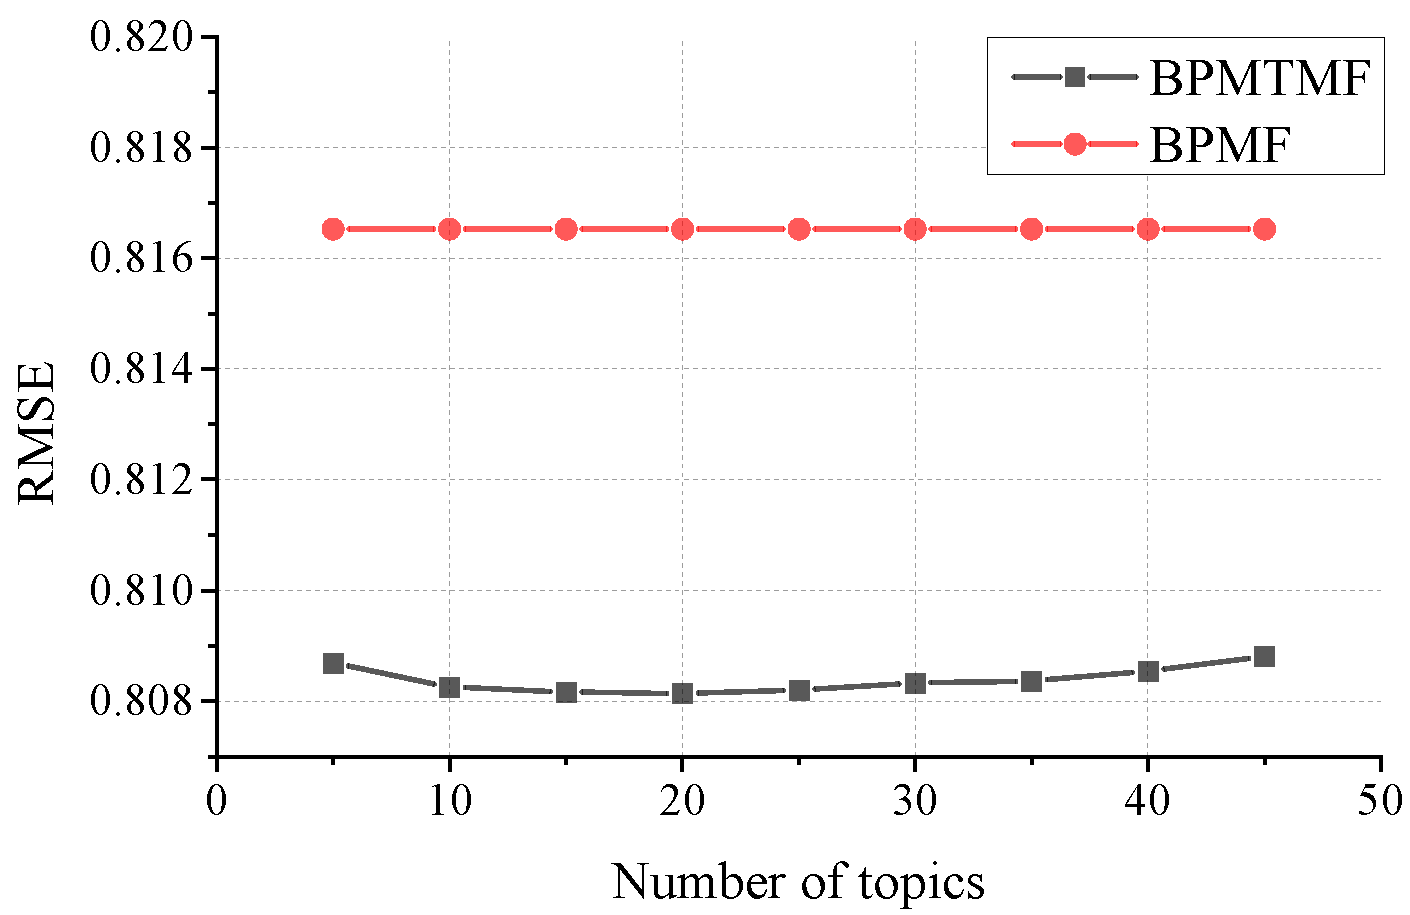
\includegraphics[width=0.75\textwidth]{Fig/bpmtmf/number}
	\caption{不同主题个数对推荐准确率的影响}
	\label{fig-bpmtmf-number}
\end{figure}
由于本章工作需要根据每个主题设置主题特定的用户隐藏特征向量和商品隐藏特征向量,因此本章提出的BPMTMF一个重要的参数是主题个数(也就是 $H$)。本小节实验以5为间隔在区间$[5,45]$上设置不同的主题个数$H$。图~\ref{fig-bpmtmf-number}展示了BPMTMF的RMSE性能。图中能观察到在主题个数符合$15\le H\le 25$时,BPMTMF取得的推荐准确率最高。作为对照,实验也测试了BPMF的性能,BPMF其实是只有一个主题的BPMTMF,是BPMTMF的一种特殊情形。可以看出,当主题个数$H=5$时,BPMTMF的推荐准确率已经远好于主题个数为1时的准确率。通过结合表~\ref{tab-bpmtmf-cluster}聚类分析能够看出利用多主题的矩阵分解模型能够有效地对用户和商品复杂的特性进行建模,从而提高预测评分的准确性。

\begin{figure}
	\centering
	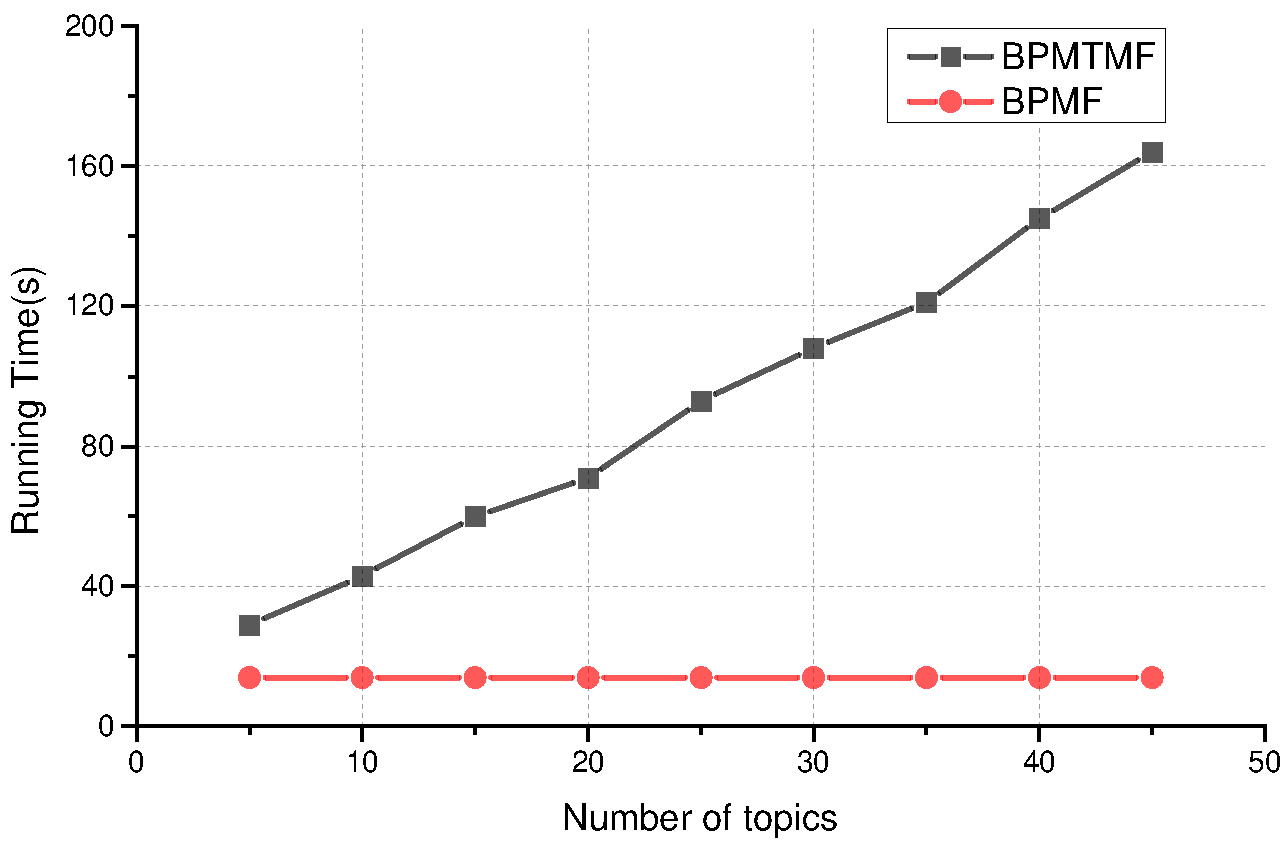
\includegraphics[width=0.75\textwidth]{Fig/bpmtmf/ktime}
	\caption{不同主题个数对模型训练时间的影响}
	\label{fig-bpmtmf-time}
\end{figure}

本小节实验同时也展示了BPMTMF每轮迭代的算法运行时间,如图~\ref{fig-bpmtmf-time}所示。该实验使用的电脑配置是Ubuntu系统,CPU为4-core Intel Xeon E5-1603 2.86GHz以及16G内存,使用Java编程语言实现BPMTMF。在之前的时间复杂度分析中,每一轮迭代本文模型BPMTMF的时间复杂度为$\mathcal{O}(KH|\mathbf{R}|+K^2|\mathbf{R}|+K^3HN+K^3HM)$。在数据集大小和隐藏特征向量维度不变的情况下,BPMTMF的时间复杂度与主题个数$H$成正比。从图~\ref{fig-bpmtmf-time}可以看出,实验结果也符合本章的时间复杂度理论分析。为了提高算法运行效率在以后工作中引入并行优化算法去加速参数学习过程。

\section{本章小结}
\label{sec-bpmtmf-conclusion}
本章提出了局部矩阵分解的概率形式,巧妙地融合概率矩阵分解和主题模型到同一个模型当中,进而提出全贝叶斯版本的概率多主题矩阵分解BPMTMF。本章同时也说明了之前一些非概率版本的局部矩阵分解模型和本章模型的紧密联系。本章工作在评分预测上能够更加有效地反映用户和商品复杂的内在特性,以及有更好的模型解释性。另外,在大规模真实数据集上的实验也表明了本章模型的有效性。

\clearpage
\phantom{s}
\clearpage
\chapter{时间感知的标签推荐}
\label{chapter-wpitf}
本章重点介绍时间感知的标签推荐研究内容。首先,章节~\ref{sec-wpitf-intro}阐述标签推荐的研究背景、意义、研究贡献。其次,章节~\ref{sec-wpitf-related}讨论与标签推荐以及模型相关的研究工作。随后,章节~\ref{sec-wpitf-wpitf}重点介绍本章提出的标签推荐模型以及相关参数学习等。章节~\ref{sec-wpitf-exp}通过实验验证模型的有效性。最后总结本章标签推荐的研究内容。


\section{引言}
\label{sec-wpitf-intro}
分众分类标签系统如Delicious、Last.fm和豆瓣等互联网服务网站允许用户使用关键字标记书签、音乐、电影等资源(或者商品),这种行为被称为标注标签。标签是Web 2.0的一个重要的特征,它可以帮助用户管理自己收藏的资源,方便用户以一种简单的机制来协同管理或搜索网络中的资源(本章节中一般描述为商品)~\cite{dellschaft2012measuring}。图~\ref{fig-wpitf-douban}展示了豆瓣电影的标签系统。左图~\ref{fig-wpitf-doubana}展示了用户对电影显式反馈时利用标签对商品描述。用户对商品标注标签不仅标明了商品的属性,也说明了用户对商品的关注点,侧面反映了用户偏好。右图~\ref{fig-wpitf-doubanb}展示了用户通过标签来寻找自己感兴趣的电影,说明标签方便用户检索信息。

\begin{figure}
	\centering
	\subfigure[对电影标注标签]{
		\label{fig-wpitf-doubana}
		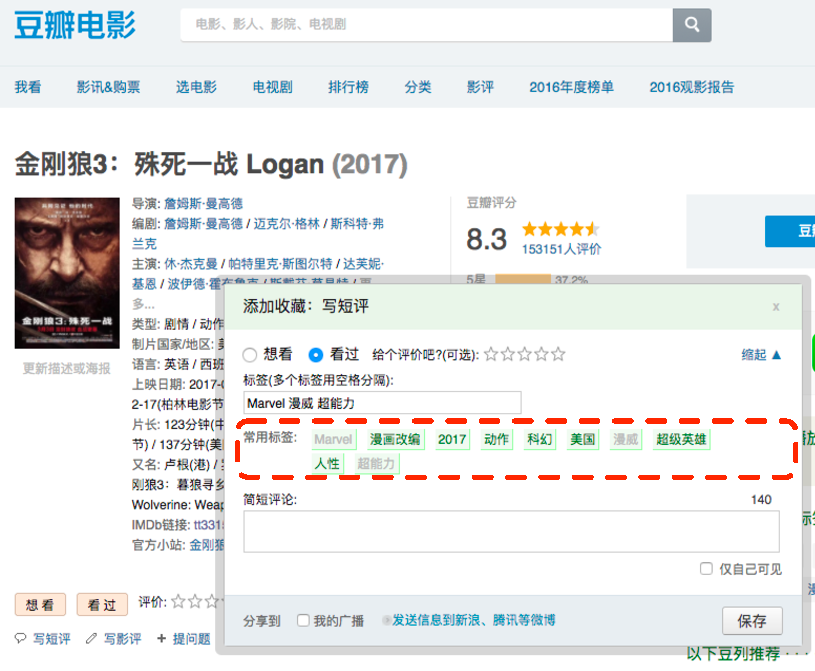
\includegraphics[width=0.45\textwidth]{Fig/wpitf/doubanTag}}
	\hspace{0.8cm}
	\subfigure[根据标签寻找电影]{
			\label{fig-wpitf-doubanb}
		
\includegraphics[width=0.45\textwidth]{Fig/wpitf/doubanTag1}}
	\caption{豆瓣电影标签例子}
	\label{fig-wpitf-douban}
\end{figure}

个人标签系统可以极大的提高网络商品的搜索效率~\cite{jaschke2008tag},同时可以准确刻画用户和商品的属性,帮助缓解冷启动问题\cite{lika2014facing},提高\textit{商品推荐}和\textit{评分预测}准确率~\cite{tso2008tag,zhen2009tagicofi,lacic2014recommending,saha2015predicting},促进推荐系统的良性循环。
但仍然有许多用户懒于给自己收藏的内容加上标签,因此需要个性化的标签推荐系统自动地给用户推荐标签,从而帮助用户更好地进行资源管理。目前的标签推荐方法分为两类:非个性化标签推荐方法和个性化标签推荐方法。非个性化的标签推荐系统针对某一资源,会给所有的用户推荐相同的标签,比如最流行标签模型,针对某一资源会给所有用户推荐目标资源上最热门的标签,这是一种非个性化的推荐。 而Rendle等人~\cite{rendle2009learning}已经验证了个性化推荐方法比理论上最优的非个性化的推荐方法的效果要好。个性化的标签推荐系统通过分析用户以往的标注标签行为来预测用户将会使用的标签,推荐结果由用户和商品属性共同决定。例如两个用户曾经对同一件商品标注过相同的标签,那么将来他们也有可能对另一商品使用相同的标签。也有可能一个用户近期大量使用某个标签,那么之后的一段时间也很可能还使用该标签对网络商品进行标记。进行个性化的推荐之所以有意义是因为对同样的资源,用户倾向于使用不同的标签,比如Last.fm提供非个性化的标签推荐,但用户仍然会使用不同的标签来标记音乐资源。

一些个性化标签推荐系统使用张量分解技术来为候选标签排序。基于张量分解的模型将用户-商品-标签张量分解成三个维度的特征矩阵,来表示与用户、商品、标签相关的隐含特征。基于Canonical分解的PITF\cite{rendle2010pairwise}张量分解方法,改进了基于Tucker分解的RTF\cite{rendle2009learning}模型复杂度与分解维度成立方比的缺点,使得模型运行时间与数据集的大小及特征维度均成线性关系,可以更好地处理高维分解,同时保持张量分解类算法较好的推荐新信息的能力,发现用户潜在的但自己尚未发现的兴趣偏好标签的优点。经典的张量分解类方法虽然有众多协同过滤的优点,但它们没有考虑到用户打标签的行为会随时间变化这一特征,以及较难处理好稀疏性、新用户冷启动等问题。因此最近出现了一些基于时间和频次的标签推荐系统BLL(Base-Level Learning)类方法,GIRP\cite{zhang2012integrating}, GIRPTM\cite{zhang2012integrating},BLL\cite{anderson2004integrated},BLLac\cite{kowald2015forgetting}等,这些方法仿照人脑存取长期记忆的方式,认为用户会倾向于再次使用自己最近最多使用过的标签。其中BLL类方法利用用户以往打标签行为与当前时间的间隔、标签的使用频次来估计用户将来重复使用某一标签的概率,并结合该网络商品中最流行标签进行推荐。但此类方法只能推荐历史记录中有的标签,没有推荐新标签的能力。

综合分析和考虑上述两类方法的优缺点,本章节提出时间感知的PITF模型(Time Aware PITF,简称TAPITF),在PITF模型的基础上增加对用户-标签-时间关系的权重以及商品-标签关系的权重,使得TAPITF模型既能考虑用户打标签行为和商品关注点随时间变化而变化的现象,也能有效地利用相似用户、相似商品、相似标签的信息,从而更好地对用户给商品标注标签的行为进行建模,提高标签推荐的准确度和新颖性。最后, 本章节在Movielens、LastFM和 Delicious三个数据集上进行了对比实验,实验结果表明本章节提出的方法在准确性上优于当前最新的标签推荐算法,同时还有较好的推荐新标签的能力。

\section{相关工作}
\label{sec-wpitf-related}
尽管在章节~\ref{chapter-related-coll}介绍了推荐系统中相关的协同过滤算法,但是它重点介绍\textit{商品推荐}和\textit{评分预测}两个任务。本小节将重点介绍个性化标签推荐的相关工作。

最简单的个性化标签推荐方法是用户最流行标签模型,给用户推荐用户自身使用最多的标签。Hotho等人~\cite{hotho2006information}提出自适应的PageRank(APR)算法,其主要思想是类似于网页的PageRank算法,即如果一个商品被重要的用户用重要的标签标注过,那么它也是个重要的商品。工作~\cite{marinho2008collaborative}使用了协同过滤思想,通过计算用户相互之间的相似度计算用户对某个商品标注标签的喜好值。Robert等人~\cite{jaschke2007tag}结合PageRank算法和用户之间的相似度,提出了FolkRank算法,使得推荐效果优于简单的基于频率的算法。张量分解模型也被广泛用于标签推荐。文章~\cite{symeonidis2008tag}使用了HOSVD模型~\cite{de2000multilinear},将三维的标签数据矩阵平铺成三个二维的矩阵,然后利用SVD算法建模用户、商品和标签隐藏特征。HOSVD模型需要对三个矩阵进行SVD分解,增加了模型训练时间,工作~\cite{rendle2009learning}提出了基于Tucker分解~\cite{tucker1966some}的张量分解模型RTF-TD,通过最大化AUC直接对标签数据进行三维分解。因为RTF-TD模型在预测标签推荐时间复杂度是隐藏特征向量维度的三次方,Rendle等人提出了PITF模型\cite{rendle2010pairwise},显式地对用户、商品、标签两两之间的关系进行建模,有效地利用相似用户、相似商品、相似标签等信息来进行标签推荐,并且将预测复杂度降为与隐藏特征向量维度成正比。NLTF~\cite{fang2015personalized},使用高斯径向基核函数以非线性方式扩展了张量分解模型,用来捕捉用户描述商品的复杂行为,期望更好地刻画用户、商品、标签的内在属性。除此之外,主题模型也被用来进行标签推荐,代表性方法有基于LDA主题模型的标签推荐系统\cite{krestel2009latent},该方法使用拥有大量标签的商品来抽取隐含的主题,然后把待标注的商品映射到相应的主题上,把属于这些主题的标签推荐给用户。

上述模型忽略了用户标注标签的行为会随时间变化这一现象\cite{yin2011temporal}。因此最近的研究工作尝试在进行标签推荐时考虑时间因素,Zhang等人\cite{zhang2012integrating}基于用户打标签行为的频次和时间提出了GIRP模型,对标签第一次被使用及最后一次被使用的时间对用户重复使用标签的概率建模。GIRPTM模型\cite{zhang2012integrating}扩展了GIRP模型,推荐时考虑了目标商品上最热门的标签,同时解决新用户冷启动问题。考虑时间的因素还有基于认知科学的BLL类模型,包括BLL$_{AC}$~\cite{kowald2015forgetting}、BLL+MP$_m$~\cite{kowald2014long}、BLL$_{AC}$+MP$_m$~\cite{kowald2015refining}、3LT+MP~\cite{kowald2015forgetting}~\cite{seitlinger2013recommending}。 BLL模型认为用户会倾向于再次使用自己最近最多使用过的标签,利用幂函数对这一行为启发式建模。BLL$_{AC}$~\cite{kowald2015forgetting}扩展了BLL,除了使用长尾分布对用户历史行为的频次和时间间隔进行建模外,还增加了关联模块(Association Component)描述目标资源的特征对用户的影响,即用户不一定总是选择自己最近最多使用过的标签,会随着目标资源的不同做出调整,但只会给用户推荐他之前使用过的标签。BLL+MP$_m$~\cite{kowald2014long}和BLL$_{AC}$+MP$_m$~\cite{kowald2015refining}分别扩展了BLL和BLL$_{AC}$,都考虑给用户推荐目标资源上最热门的标签。 3LT+MP模型~\cite{seitlinger2013recommending}除了利用用户对标签的遗忘规律,还使用LDA来模仿用户存取记忆时访问的语义场,以便更好地刻画用户画像和商品属性,提高推荐的准确度。

本章节工作中对时间信息的建模方法与BLL类模型相比主要区别是:BLL类方法利用幂函数叠加的方式计算用户每次使用标签的影响,当前时间改变后需要根据当前时间与用户每次访问该标签的时间重新计算喜好值,而本章节中从时间点过程(Temporal Point Process)对时间信息建模角度出发,利用指数函数将其从叠加转化为递归形式,使得计算当前时间下用户对标签的喜好值只跟上次使用标签的时间有关,极大地减少了计算时间。

%(2)标签是用户对商品的关注点描述,用户会随着时间的变化对商品的关注也不同,因此本章节工作认为商品被标注的标签也是随着时间的变化而变化,需要使用类似于建模用户标注标签的方法对该情况建模,而BLL类方法在对商品-标签建模时只是简单地统计全部数据中商品标签的频率信息,既没有考虑时间信息对商品标签的影响,同时包含目标用户在目标商品上标注目标标签的时间之后的其他用户在该商品上使用该标签次数信息也是不合理的。

%\section{模型基础知识}
%\label{sec-wpitf-basic}


%\subsection{BLL+MP$_i$模型}
%BLL+MP$_i$~\cite{kowald2014long}使用用户以往打标签行为的频次(Frequency)及历史打标签行为时间与当前时间的间隔(Recency)来建模,同时考虑了目标资源上最热门的标签对用户的影响。
%
%首先根据某个标签被目标用户使用的记录来计算标签的活跃程度BLA(Base-Level Activation):
%\begin{equation}
%BLA(t,u)=\ln (\sum_{i=1}^{n}(s_{ref}-s_{j})^{-d})
%\end{equation}
%其中$n$是标签$t$被用户$u$使用的总次数,第$j$次的时间戳 为$s_j$,$s_{ref}$表示用户当前要打标签的时间,时间间隔是两者的差值\footnote{ 原论文BLL代码: \url{https://github.com/learning-layers/TagRec/} 使用的是两者时间戳的差值$+1.0$,且时间戳以秒为单位。},d的取值为0.5\cite{anderson2004integrated}。经过归一化处理后:
%\begin{equation}
%||BLA(t,u)||=\frac{\exp (BLA(t,u))}{\sum_{t'=1}^{m}\exp (BLA(t',u))}
%\end{equation}
%其中$m$表示用户$u$使用过的标签的总数。
%
%除此之外该模型还考虑了用户当前所处上下文中的语义提示信息,即MP$_i$,表示的是目标资源$i$上最热门的标签。给定用户-资源对$(u,i)$,推荐标签预测分数可以下公式计算:
%\begin{equation}
%\hat{y}_{u,i,t}=\beta ||BLA(u,t)||+(1-\beta)|||Y_{t,i}|||
%\end{equation}
%$\beta$为调节用户-标签和资源-标签偏好的权重,当$\beta=0.0$时模型退化为MP$_i$模型,当$\beta=1.0$时模型变为基本的BLL模型,$|Y_{t,i}|$表示目标资源$i$在标签$t$上的数量。


\section{时间感知的逐对排序张量分解模型}
\label{sec-wpitf-wpitf}
本章节主要介绍时间感知的标签推荐模型。本小节首先介绍利用时间点过程中的Hawkes过程对用户给商品标注标签的时间信息建模。因为原始Hawkes过程是一个累加过程,需要随着时间推移需要重新计算,本章工作针对这一缺点将其改进成一个递归形式,降低预测标签喜好值的计算时间复杂度。然后,本章工作将时间建模信息以权重的方式与张量分解模型结合得到时间感知的PITF模型(Time Aware PITF,简称TAPITF)。章节中未介绍的符号说明详见章节~\ref{sec-c2-basic}中表~\ref{tab-basic-notation}。下面开始具体地介绍TAPITF模型。

\subsection{时间信息建模}
\label{sec-wpitf-time}
时间点过程~\cite{schoenberg2010introduction}是描述时序关系离散事件的随机过程。例如用户标注标签中,每个点表示用户在某一时刻标注标签,每个点以时间顺序排列,通过点之间的时间间隔描述整个点过程。本章节工作利用时间点过程中\textbf{Hawkes过程}~\cite{hawkes1971spectra}对标签时间信息建模。Hawkes过程是泊松过程的非马尔科夫扩展,表现一种``自我激励''的过程,每次事件的发生影响未来时间段事件的重新发生。Hawkes过程的条件强度定义如下:

\begin{equation}
\label{equ-wpitf-hawkes}
\tau(s) = \tau_0 + \sum_{s_i<s}E(s,s_i)
\end{equation}
其中$E(s,s_i)\geq 0$是用来描述时间间隔的激励函数,$\tau_0$是初始强度。用户一般会在连续一段时间内访问某类相似商品,会使用相同的标签描述商品特性。另外,因为用户的个人语言习惯,有多个词表示同一个意思(例如``风景''和``景色")时,用户偏向使用自己熟悉的词。因此,用户偏向使用近期较多使用的标签,符合上述``自我激励''的Hawkes过程。本章节工作利用上述Hawkes过程的条件强度来拟合用户使用标签的行为。

\begin{figure}
	\centering
	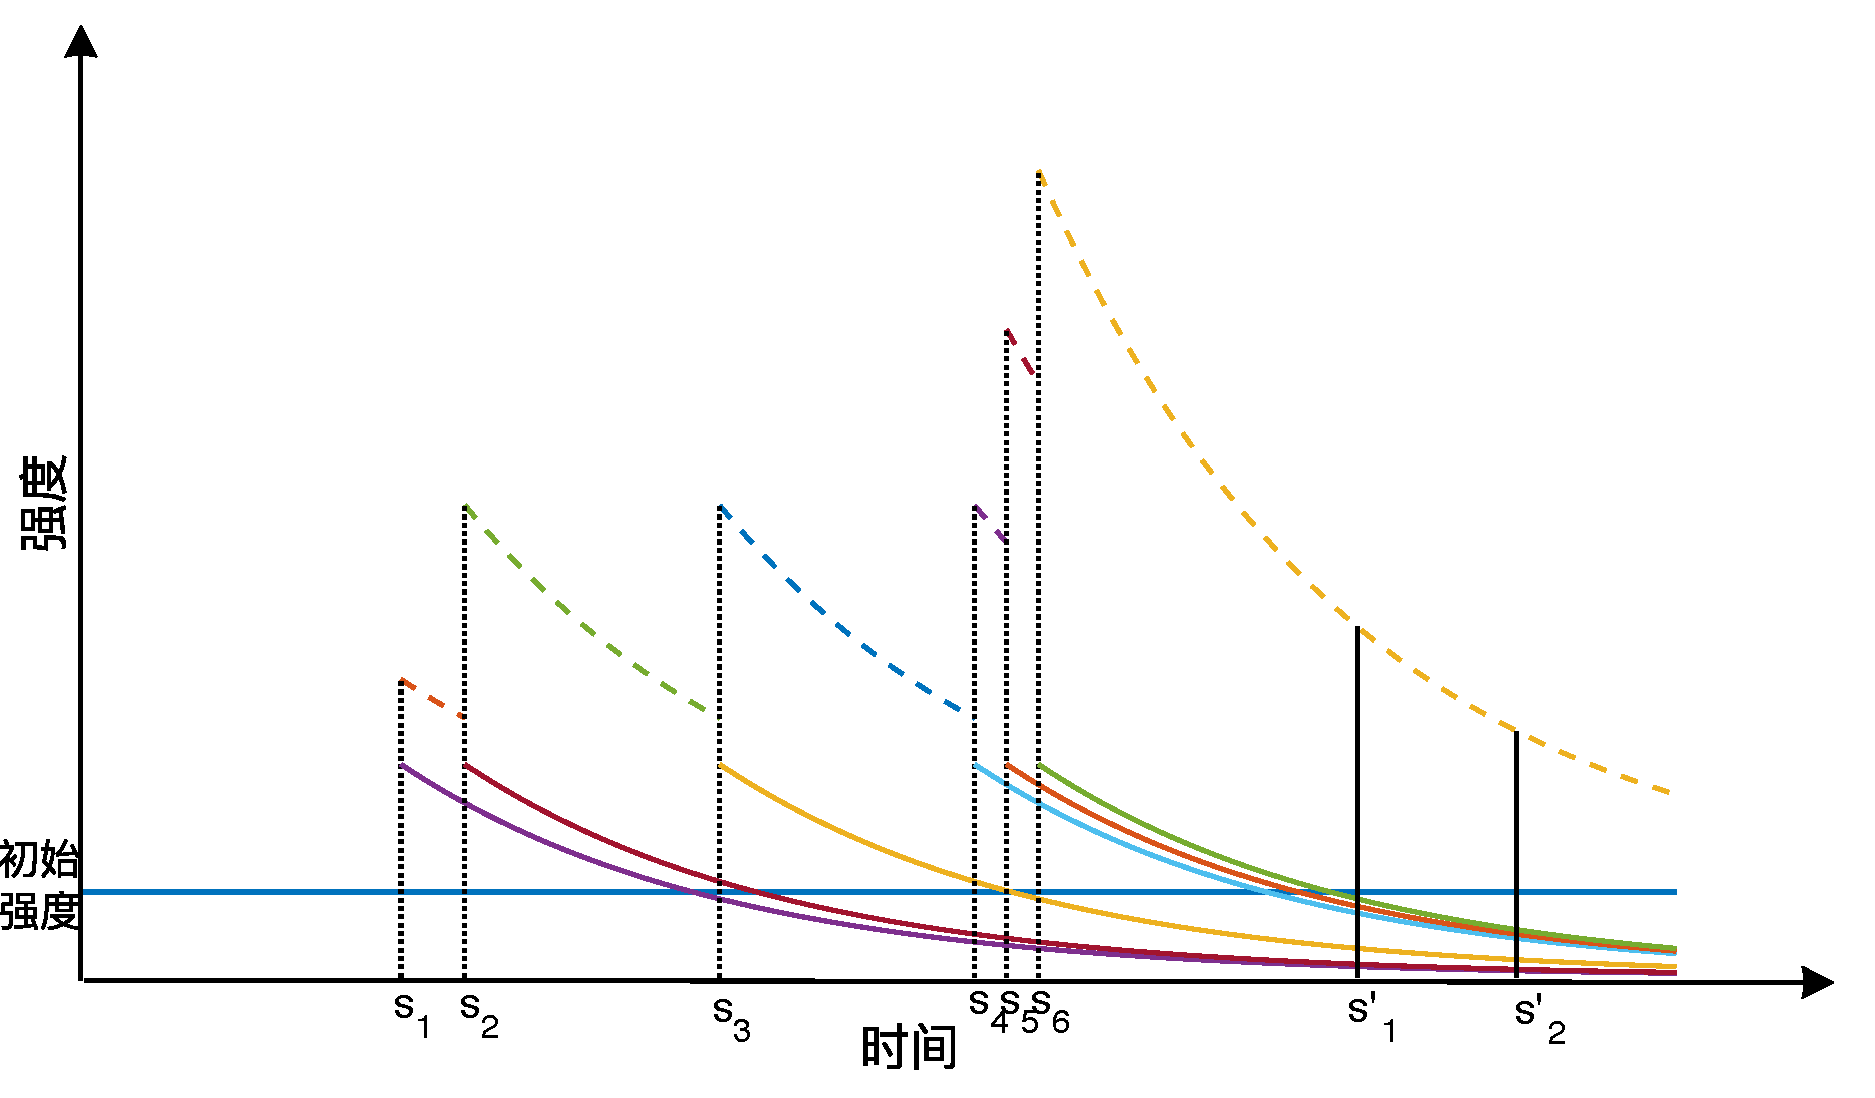
\includegraphics[width=0.9\textwidth]{Fig/wpitf/tagHawkes}
	\caption{Hawkes过程的条件强度函数示例}
	\label{fig-wpitf-tagHawkes}
\end{figure}

如果$\tau_0=0$以及激励函数设置为幂函数$E(s,s_i)=(s-s_i)^{-d}$,其中$d$是强度参数,那么这个函数等同于BLL类论文~\cite{kowald2014long,kowald2015forgetting,kowald2015refining}中对时间建模的函数。本章节工作中激励函数不同于上述设置,而是使用了指数函数$E(s,s_i)=\exp^{-d(s-s_i)}$。本章节工作使用指数函数作为激励函数一方面是因为幂函数和指数函数对最终标签推荐性能相差不大,另一方面主要是指数函数通过变化可以将叠加形式转换为递归形式,极大降低算法复杂度,特别是后面小节与PITF模型结合后参数学习的复杂度。图~\ref{fig-wpitf-tagHawkes}展示了激励函数为指数函数的Hawkes过程条件强度函数示例,其中$s_1, s_2,..., s_6$是事件发生的时间戳,彩色实线是每次事件发生后对未来事件的影响值,彩色虚线表示所有过去事件对未来事件的影响,任务是计算在$s'_1$和$s'_2$时刻的强度值。可以发现,每次事件发生都会增加未来时间发生率,并且随着时间的增加,影响越来越少。根据公式~\ref{equ-wpitf-hawkes},得到$s'_1$时刻的强度值需要计算并求和之前6次事件发生时间到$s'_1$的激励值,之后计算$s'_2$时刻的强度值又需要重新计算6次。也就是说每次计算某一时刻某个时间可能发生的强度值,都需要计算该时刻之前发生的所有事件对现在的影响。而指数函数作为激励函数,可以将加和形式转化为递归形式,还是图~\ref{fig-wpitf-tagHawkes}的例子,计算$s'_1$时刻激励函数之和$\tau^*(s'_1)$如下转化:

\begin{align}
\tau^*(s'_1) &= \sum_{i=1}^6E(s'_1,s_i)=\sum_{i=1}^6 \exp^{-d(s'_1-s_i)}\nonumber\\
&=\exp^{-d(s'_1-s_6)}\big(1+ \sum_{i=1}^5\exp^{-d(s_6-s_i)}\big)\nonumber\\
&=\exp^{-d(s'_1-s_6)}\big(1+\tau^*(s_6)\big)
\end{align}
可以发现是$s'_1$时刻事件发生的强度值只跟前一个事件发生$s_6$时刻的强度值有关。该现象说明只要预先计算完成所有事件发生时刻的强度值,任意时刻$s$的强度值只需要根据在$s$之前离$s$最近的事件发生时的强度即可求得。具体地,第$u$个用户在时刻$s$使用第$t$个标签的强度为:
\begin{equation}
\label{equ-wpitf-hawkes-user}
\tau(u,t,s) = \sum_{s_i<s} \exp^{-d(s-s_i)}= \exp^{-d(s-s_{last})}\big(1+\tau(s_{last})\big)
\end{equation}
其中$\tau_0=0$,$s_{last}$指的是离$s$最近的事件发生的时间。

\subsection{模型构建与学习}
从BLL类论文中可以发现利用用户打标签的时间戳信息建模,模拟用户倾向于再次使用自己最近最多使用过的标签的行为,同时考虑了目标资源最热门的标签,解决新用户冷启动问题,在标签推荐情境下能有较高的准确率。然而此类方法只能够推荐用户本来就熟悉的标签或者是目标商品最热门的标签,完全没有推荐新标签的能力。而张量分解模型是协同过滤的推荐方法,具有协同过滤方法的优点,譬如有推荐新信息的能力,发现用户潜在的但自己尚未发现的兴趣偏好标签等。然而此类模型缺少了时间和内容信息,没有对用户标签记忆模式建模,以及在冷启动情况下推荐效果不佳。

因此,本文综合考虑上述两类模型的优缺点,提出时间感知的的逐对张量分解模型(Time Aware PITF,简称TAPITF),其对用户-商品$<u,m>$的预测值如下:

\begin{equation}
\label{eq-wpitf-prediction}
\hat{y}_{umt}^s=w_{ut}^{s}\mathbf{P}_u^\top\mathbf{T}_t^{\mathcal{P}}+w_{mt}\mathbf{Q}_m^\top\mathbf{T}_t^{\mathcal{Q}}
\end{equation}
其中$w_{u,t}^s$是用户-标签-时间$<u,t,s>$权重,$w_{i,t}$是商品-标签对$<m,t>$权重。当第$u$个用户在时间$s$之前标注第$t$个标签的次数越多,且时间越近,那么用户-标签-时间$<u,t,s>$权重$w_{ut}^s$越大。类似地,所有用户在第$m$个商品标注第$t$个标签$t$的次数越多,那么商品-标签对$<m,t>$权重越大。同时需要保证当第$u$个用户在时间$s$前未标注过第$t$个标签时(或者没有用户在第$m$个商品上标注过第$t$个标签),权重$w_{ut}^s$和$w_{mt}$大于零以保证在历史记录中未出现过但相关的标签也能有机会被推荐给目标用户和目标商品。因此,针对权重$w_{ut}^s$,利用上一小节对时间建模信息的公式~\ref{equ-wpitf-hawkes-user}:

\begin{equation}
\label{eq-weight-uts1}
w_{ut}^s =1 + \log_{10}(1+10^{a^\mathcal{P}}\cdot ||\tau(u,t,s)||)
\end{equation}	
其中常数$\alpha^\mathcal{P}$是控制权重的增长速率。$||\tau(u,t,s)||$表示经过归一化的数值$||\tau(u,t,s)|| = \frac{\tau(u,t,s)}{\sum_{t\in \mathcal{T}_u}\tau(u,t,s)}$,$\mathcal{T}_u$表示第$u$个用户使用过的标签集合。当$||\tau(u,t,s)||$越大时,$w_{ut}^s$越大,且$||\tau(u,t,s)||=0$时,$w_{ut}^s=1$,也就是说第$u$个用户在时间$s$前未标注过第$t$个标签时,权重都为1。而针对权重$w_{mt}$,类似于BLL+MP$_m$~\cite{kowald2014long},本章工作利用商品最流行标签建立相应权重:


\begin{equation}
\label{eq-weight-it} w_{mt} = 1+\log_{10}(1+10^{a^\mathcal{Q}}\cdot \||\hat{\mathbf{Y}}_{mt}|\|)
\end{equation}
其中常数$\alpha^\mathcal{Q}$是控制权重的增长速率,$|\hat{\mathbf{Y}}_{mt}|$代表第$m$商品被第$t$个标签标记的次数。另外目标函数 Eq.~\ref{eq-wpitf-prediction}中$\mathbf{P}_u^\top\mathbf{T}_t^{\mathcal{P}}$(或者$\mathbf{Q}_m^\top\mathbf{T}_t^{\mathcal{Q}}$)继承了PITF的方法,能够较好地刻画用户、商品、标签三者的潜在向量特征,能够发现用户喜好(或者商品相关)但未发现的标签,提高推荐的新颖性。

 \begin{algorithm}
	\renewcommand\baselinestretch{1.3}\selectfont 	
	\begin{algorithmic}[1]
		\caption{TAPITF优化算法}
		\label{algo-tfwpitf-opt}
		\REQUIRE{用户对商品打标签历史记录$\{<u,m,t,s>\}$,隐藏向量维度$K$,学习速率$\iota$,正则化参数$\lambda$;}
		\ENSURE{用户隐藏特征向量$\mathbf{P}\in \mathbb{R}^{N \times K}$,商品隐藏特征向量$\mathbf{Q}\in \mathbb{R}^{M\times K}$,以及对应的标签隐藏特征向量$\mathbf{T}^\mathcal{P}\in \mathbb{R}^{T\times K}, \mathbf{T}^\mathcal{Q}\in \mathbb{R}^{T\times K}$;}
		
		\STATE {统计时间,频次,计算每条历史记录$y=<u,m,t,s>$的用户-标签-时间权重$w_{ut}^s$以及商品-标签权重$w_{mt}$;}
		\STATE {使用高斯分布$N(0,0.01)$初始化$\mathbf{P}, \mathbf{Q}, \mathbf{T}^\mathcal{P}, \mathbf{T}^\mathcal{Q}$;}
		
		\REPEAT 
		\STATE {从训练集中均匀采样$y=<u,m,t_A,s_A>$和对应的负样本标签$t_B$;}
		\STATE {根据$<u,t,t_B,s_A>$计算负样本的用户-标签权重$w_{ut_B}^{s_A}$;}
		\STATE {$\hat{y}_{umt_At_B}\leftarrow \hat{y}_{umt_A}-\hat{y}_{umt_B}$}
		\STATE {$\delta \leftarrow (1 - \sigma(\hat{y}_{umt_At_B}))$}
		
		\FOR{ $k$ from $1$ to $K$} 
		
		\STATE {$\mathbf{P}_{uk}\leftarrow \mathbf{P}_{uk}+\iota\cdot (\delta \cdot (\hat{w}_{ut_A}^{s_A}\cdot \mathbf{T}^\mathcal{P}_{t_Ak}-\hat{w}_{ut_B}^{s_A}\cdot \mathbf{T}^\mathcal{Q}_{t_Bk})-\lambda \cdot \mathbf{P}_{uk})$} 
		
		\STATE {$\mathbf{Q}_{mk}\leftarrow \mathbf{Q}_{mk}+\iota \cdot (\delta \cdot(\hat{w}_{ut_A}^{s_A}\cdot \mathbf{T}^\mathcal{P}_{t_Ak}-\hat{w}_{ut_B}^{s_A}\cdot \mathbf{T}^\mathcal{Q}_{t_Bk})-\lambda \cdot \mathbf{Q}_{mk})$}
		
		\STATE {$\mathbf{T}^\mathcal{P}_{t_Ak}\leftarrow \mathbf{T}^\mathcal{P}_{t_Ak}+\iota \cdot (\delta \cdot \mathbf{P}_{uk}\cdot w_{ut_A}^{s_A}-\lambda \cdot \mathbf{T}^\mathcal{P}_{t_Ak})$}
		
		\STATE {$\mathbf{T}^\mathcal{P}_{t_Bk}\leftarrow \mathbf{T}^\mathcal{P}_{t_Bk}+\iota \cdot (\delta \cdot (-\mathbf{P}_{uk})\cdot w_{ut_B}^{s_A}-\lambda \cdot \mathbf{T}^\mathcal{P}_{t_Bk})$}
		
		\STATE {$\mathbf{T}^\mathcal{Q}_{t_Ak}\leftarrow \mathbf{T}^\mathcal{Q}_{t_Ak}+\iota \cdot (\delta \cdot \mathbf{Q}_{mk}\cdot w_{mt_A}-\lambda \cdot \mathbf{T}^\mathcal{Q}_{t_Ak})$}
		
		\STATE {$\mathbf{T}^\mathcal{Q}_{t_Bk}\leftarrow \mathbf{T}^\mathcal{Q}_{t_Bk}+\iota \cdot (\delta \cdot (-\mathbf{Q}_{mk})\cdot w_{mt_B}-\lambda \cdot \mathbf{T}^\mathcal{Q}_{t_Bk})$}
		\ENDFOR		
		\UNTIL{收敛}		
		
		\RETURN {$\mathbf{P}, \mathbf{Q}, \mathbf{T}^\mathcal{P}, \mathbf{T}^\mathcal{Q}$}	
	\end{algorithmic}
\end{algorithm}

TAPITF使用BPR框架进行最大化成对排序目标函数,采用负采样随机梯度下降算法进行迭代优化,具体如算法~\ref{algo-tfwpitf-opt}所示。首先,在循环迭代之前,根据训练集标注标签的时间和频次统计,计算每条历史记录$y=<u,i,t,s>$中的用户-标签-时间$<u,t,s>$权重$w_{ut}^s$以及所有商品-标签对$<m,t>$的权重$w_{mt}$(第1行)。然后使用高斯分布分别初始化用户、商品、标签隐藏特征向量$\mathbf{P}, \mathbf{Q}, \mathbf{T}^\mathcal{P}, \mathbf{T}^\mathcal{Q}$(第2行)。每次迭代中,需要正样本和相应的负样本标签采样。因为正样本用户-标签-时间$<u,t,s>$权重$w_{ut}^s$和所有商品-标签对$<m,t>$的权重$w_{mt}$预先计算好了,所以只需计算负样本标签的用户-标签-时间$<u,t_B, s_A>$权重$w_{u,t_{B}}^{s_A}$。最后根据随机梯度下降公式进行迭代优化潜在向量(第3-15行)。


\subsection{时间复杂度分析}
\label{subsec-wpitf-timeAnalysis}
因为每条历史记录$y=<u,m,t,s>$中的用户-标签-时间$<u,t,s>$权重$w_{ut}^s$以及所有商品-标签对$<m, t>$的权重$w_{mt}$在迭代优化之前已经预先计算好,所以每次迭代只要计算负样本标签的用户-标签-时间$<u,m,t_B,s_A>$权重$w_{ut_B}^S$。因此每次迭代,复杂度相对于PITF(PITF每次迭代的复杂度为$O(K)$)来说多了计算$w_{ut_B}^{s_A}$的时间, 而计算权重$w_{ut_B}^{s_A}$又跟负采样的标签有关。由公式E.q.~\ref{eq-weight-uts1}和负样本采样方法中可以看出,$w_{ut_B}^{s_A}$的计算跟第$u$个用户,标注第$t_A$个正样本标签的时间$s_A$,第$u$个用户之前打过的标签,负样本标签$t_B$这几个方面有关。所以每次计算负样本用户-标签-时间$<u,m,t_B,t_A>$权重分两种情况:(1)负样本标签$t_B$不在第$u$个用户打过的标签集合中$\mathcal{T}_u$出现过,那么不需要计算,权重$w_{ut_B}^{s_A}=1$;(2)如果负样本标签$t_B$在第$u$个用户打过的标签集合中$\mathcal{T}_u$出现过,那么根据章节~\ref{sec-wpitf-time}分析,只需要二分搜索找到时间$t_A$之前第$u$个用户最近使用标签$t_B$的时间和预先计算好的权重即可得到负样本权重$w_{ut_B}^{s_A}$,因此复杂度为$O(\log(n_{ut_B}))$,$n_{ut_B}$代表第$u$个用户使用第$t_B$个标签的次数。这里假设每个历史记录循环迭代一遍,那么每条记录迭代计算$w_{ut_B}^{s_A}$的复杂度期望跟标签被使用的平均次数相关。因此,在最坏的情况下,也就是每次负采样的标签都是用户所使用过的标签,每次采样迭代的时间复杂度为$O(K+\log(n_{ut_B}))$。可以看出,如果数据集比较稠密的情况下,TAPITF每次迭代的运行时间会比PITF高一些。考虑到真实世界网络海量数据的稀疏性,TAPITF每次迭代的运行时间对比于PITF的运行时间增加的时间是有限的,在可接受的范围之内。

\section{实验及分析}
\label{sec-wpitf-exp}
本小节将介绍实验中用到的数 据集、实验设置、度量指标、评估方法以及实验结果。

\subsection{实验设置}

\subsubsection{数据集}
本实验中采用了三种互联网上可免费获取的标签数据集: Movielens、LastFM、Delicious\footnote{\url{http://files.grouplens.org/datasets/hetrec2011}}。三个数据集来自不同的领域,其中 Movielens 是一个电影推荐系统网站,LastFM 是一个网络电台和音乐社区,Delicious 则是一个书签网站。三个数据集的统计信息如表\ref{tab-wpitf-datasets}所 示,其中$U$表示用户-商品对数目,$U/M$体现数据集的稀疏程度。core定义了对数据集的过滤程度。$p$-core 表示数据集中的用户、商品以及标签在所有用户-资 源对中都至少出现$p$次。实验中选取了no core(完整数据集)和 core 3 两种情况。


% Table generated by Excel2LaTeX from sheet '工作表1'
\begin{table}[H]
  \centering
  \caption{标签数据集Movielens,LastFM和Delicious的统计信息}
      	  \label{tab-wpitf-datasets}
    \begin{tabular}{|c||c|c|c|c|c|c|}
    \hline
    \multicolumn{1}{|l||}{ } & \multicolumn{1}{l|}{core } & \multicolumn{1}{l|}{$N$ } & \multicolumn{1}{l|}{$M $} & \multicolumn{1}{l|}{$T$ } & \multicolumn{1}{l|}{$U$ } & \multicolumn{1}{l|}{$U/M$} \bigstrut\\
    \hline
    \hline
    \multirow{2}[4]{*}{Movielens } & -     & 2,113 & 5,908 & 9,079 & 27,712 & 4.69 \bigstrut\\
\cline{2-7}          & 3     & 656   & 2,376 & 2,061 & 18,427 & 7.76 \bigstrut\\
    \hline
    \multirow{2}[4]{*}{LastFM } & -     & 1,892 & 12,523 & 9,749 & 71,064 & 5.68\bigstrut \\
\cline{2-7}          & 3     & 1,277 & 5,940 & 2,761 & 59,692 & 10.05 \bigstrut\\
    \hline
    \multirow{2}[4]{*}{Delicious } & -     & 1,867 & 69,223 & 40,897 & 104,799 & 1.51 \bigstrut\\
\cline{2-7}          & 3     & 1,458 & 5,074 & 4,233 & 20,543 & 4.05 \bigstrut\\
    \hline
    \end{tabular}%
\end{table}%


\subsubsection{参数设置}
为了评价本章节提出的标签推荐模型,实验采用“留一 法”将数据集切分为训练数据集和测试数据集。当用户打过标签的商品数唯一时,则默认将这个用户-商品对放入训练集中。

在参数设置上,BLL+MP$_m$与BLL$_{AC}$+MP$_m$与\cite{kowald2014long}设置一样,权重因子$\beta=0.5, d=0.5$,时间以秒为单位;PITF与\cite{rendle2010pairwise}中设置一样,隐含维度$K=64$,正则化因子$\lambda=0.00005$,学习速率为0.05。本章模型中$d=0.005$,时间以天为单位, 隐含维度和正则化因子与PITF设置一样。PITF和TAPITF迭代轮数均为100轮。

\subsubsection{度量标准}
为了模拟真实世界标签推荐的环境,实验从两个维度去评估算法的性能:
\begin{itemize}
	\item \textbf{准确度:}准确度是推荐系统离线评测指标中最重要的一个。常见的指标有精准率(Precision)、召回率 (Recall)以及 F1 值,公式如下:
	\begin{eqnarray}
	\label{eq-wpitf-precision}
	Prec(S_{test},n)&=&\arg_{(u,m)\in P_{S_{test}}}\frac{|Top(u,m,n)\bigcap \{t|(u,m,n)\in S_{test}\}|}{n}\\
	\label{eq-wpitf-recall}
	Rec(S_{test},n)&=&\arg_{(u,m)\in P_{S_{test}}}\frac{|Top(u,m,n)\bigcap \{t|(u,m,t)\in S_{test}\}|}{|\{t|(u,m,t)\in S_{test}\}|}\\
	\label{eq-wpitf-f1}
	F1(S_{test},n)&=&\frac{2 \cdot	Prec(S_{test},n)\cdot Rec(S_{test},n)}{	Prec(S_{test},n)+Rec(S_{test},n)}
	\end{eqnarray}
	如果没有特别说明,实验使用 F1@5 衡量准确度。
	\item \textbf{新颖性:} 实验使用\cite{belem2013exploiting}中的 AIP@10 来定义推荐的标签列表的新颖性。如果推荐的标签从没标注过目标商品,则认为这个推荐是新颖的,所以对于目标商品,如果推荐的标签的流行程度越低,则新颖性越高。
\end{itemize}

\subsubsection{对比方法}
\begin{itemize}
\item \textbf{MP$_{m}$}:方法对给定目标资源会推荐该商品下最受欢迎的标签。
\item \textbf{PITF}~\cite{rendle2010pairwise}:由 Rendle 和 Schmidt-Thieme 提出的一种改 进的张量分解模型,显式地为用户、商品以及标签之 间的两两相互作用建模。
\item \textbf{BLL+MP$_m$}~\cite{kowald2014long}:将 BLL 与 MP$_m$ 结合,BLL 部分利用用户以往标注标签行为与当前时间的间隔、标签的使用频次来估计用户将来重复使用某一标签的概率。
\item \textbf{BLL$_{AC}$+MP$_m$}~\cite{kowald2015refining}:与 \textbf{BLL+MP$_m$} 类似,但是在 BLL 上 加入关联模块,描述目标商品的特征对用户的影响。 根据\cite{kowald2015evaluating}中标签推荐标准测试,该方法是当前准确度最好的标签推荐方法。
\end{itemize}

\subsection{实验结果及分析}
实验首先研究权重因子$\alpha$对 TAPITF 准确度的 影响,然后详细的对比 TAPITF 与其他标签推荐方法 的性能差异,最后从迭代的收敛速度以及算法运行时 间上对比 TAPITF 与 PITF 的差异。

\begin{figure}
	\centering
	\subfigure[Movielens (no core)]{
		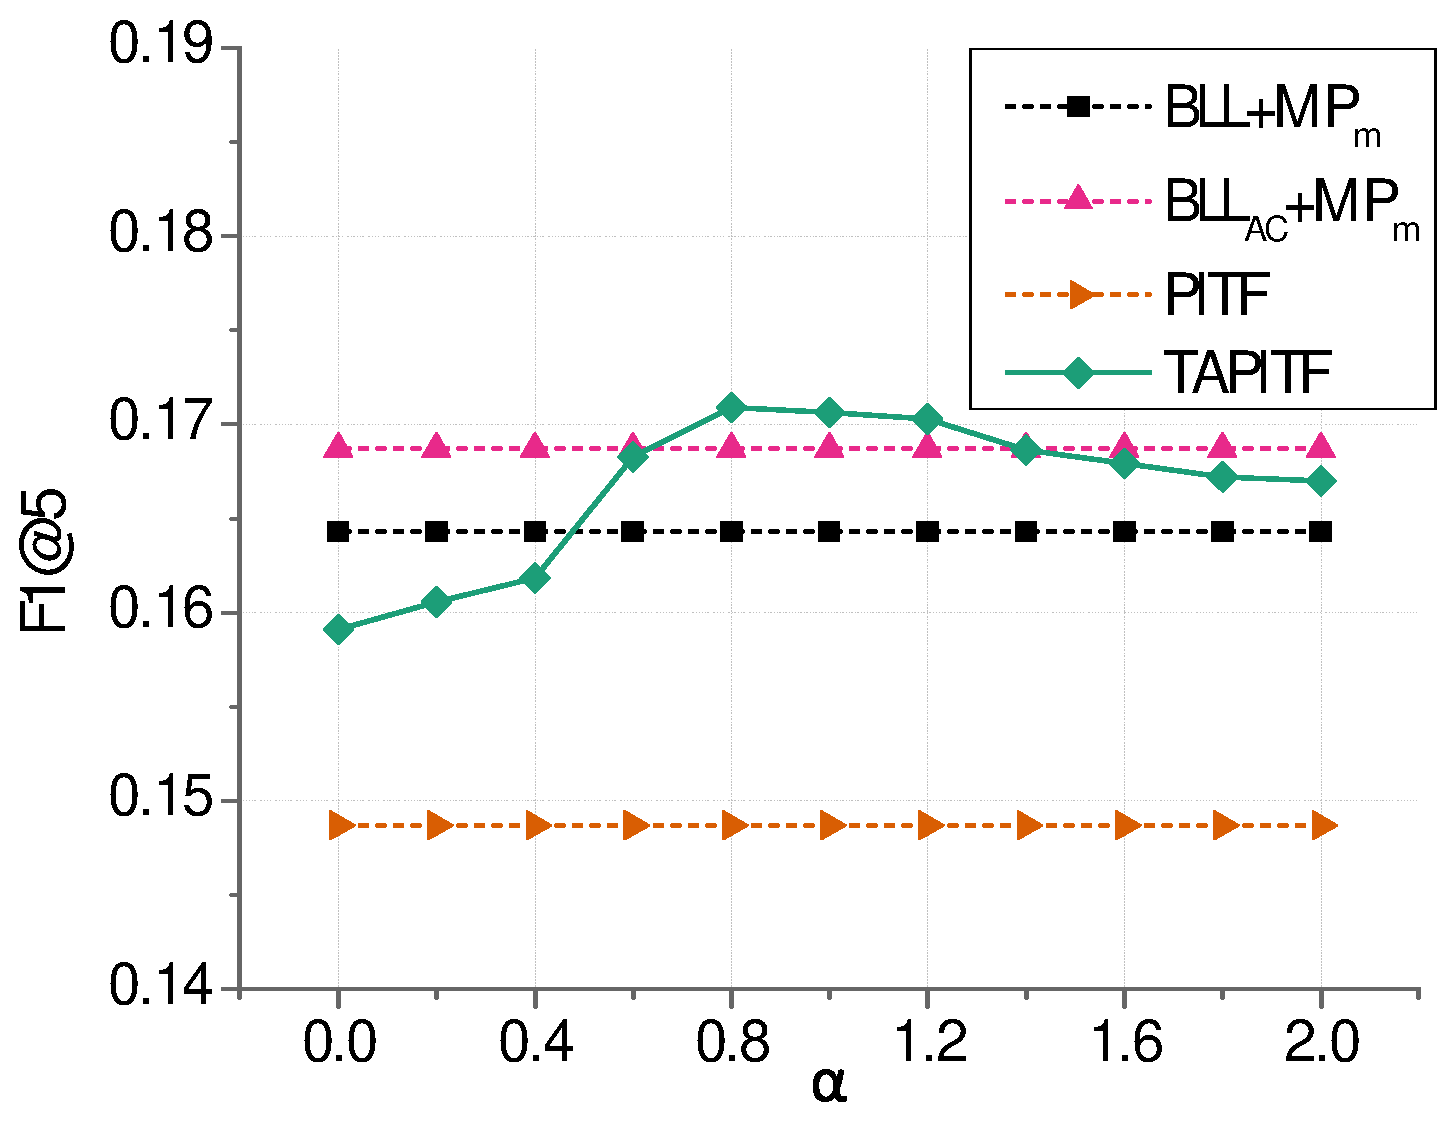
\includegraphics[width=0.485\textwidth]{Fig/wpitf/alpham1}}
	\hspace{0.0cm}
	\subfigure[Movielens (core 3)]{
		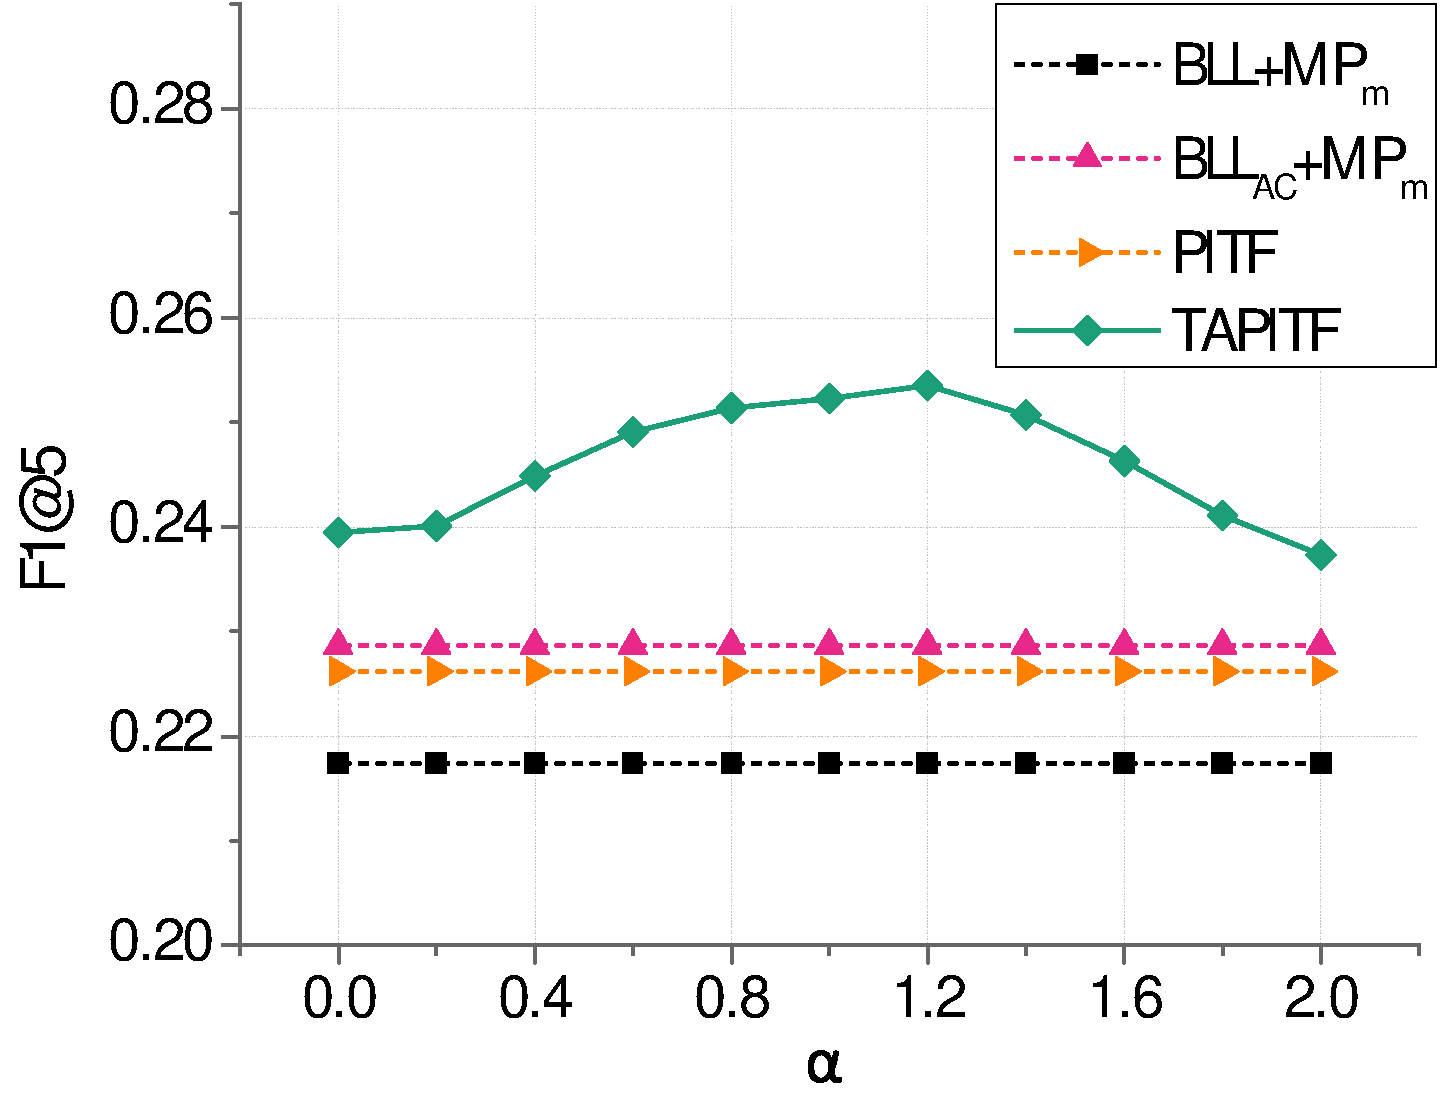
\includegraphics[width=0.485\textwidth]{Fig/wpitf/alpham3}}
	\subfigure[LastFM (no core)]{
		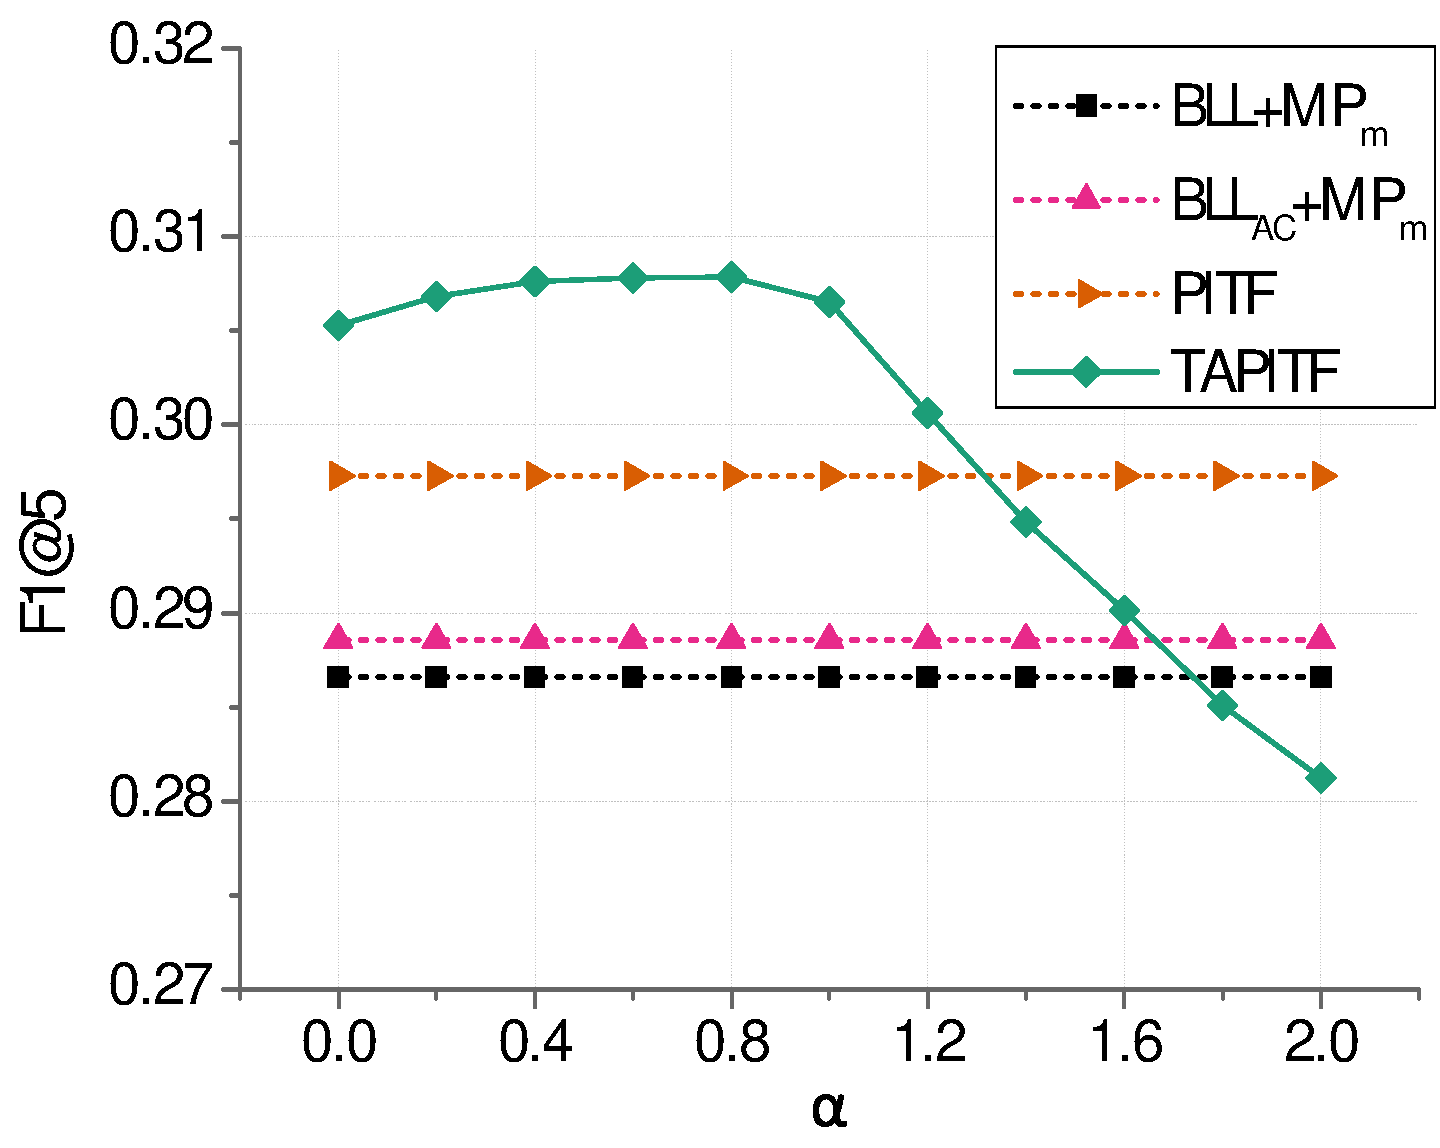
\includegraphics[width=0.485\textwidth]{Fig/wpitf/alphal1}}
	\hspace{0.0cm}
	\subfigure[LastFM (core 3)]{
		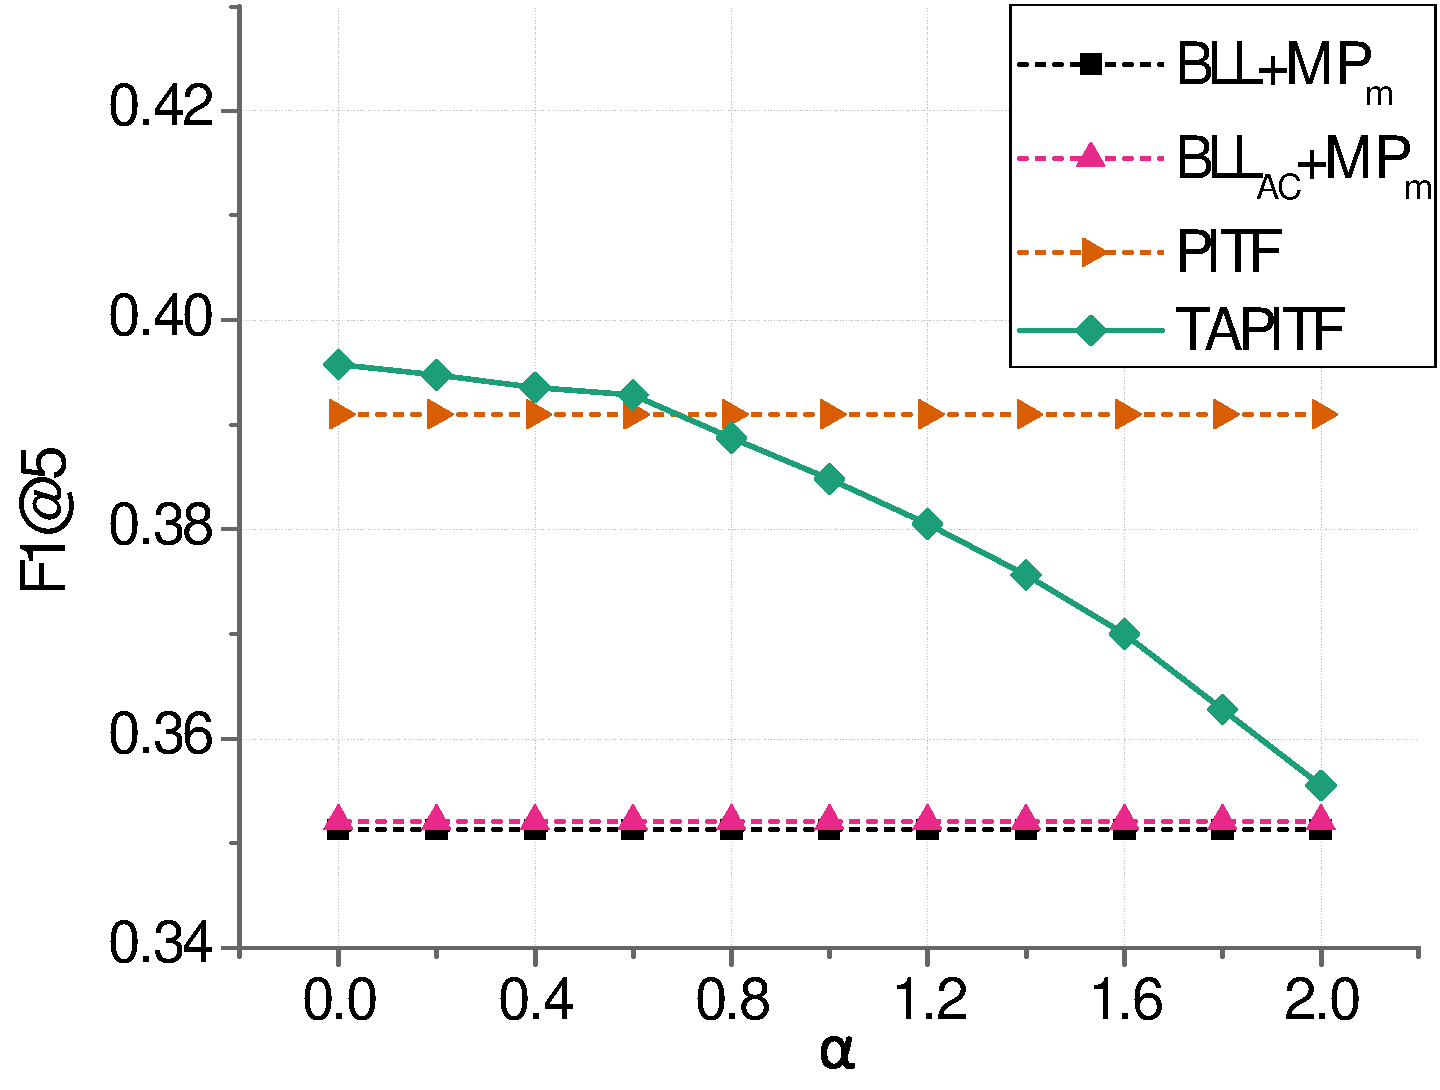
\includegraphics[width=0.485\textwidth]{Fig/wpitf/alphal3}}
	\subfigure[Delicious (no core)]{
		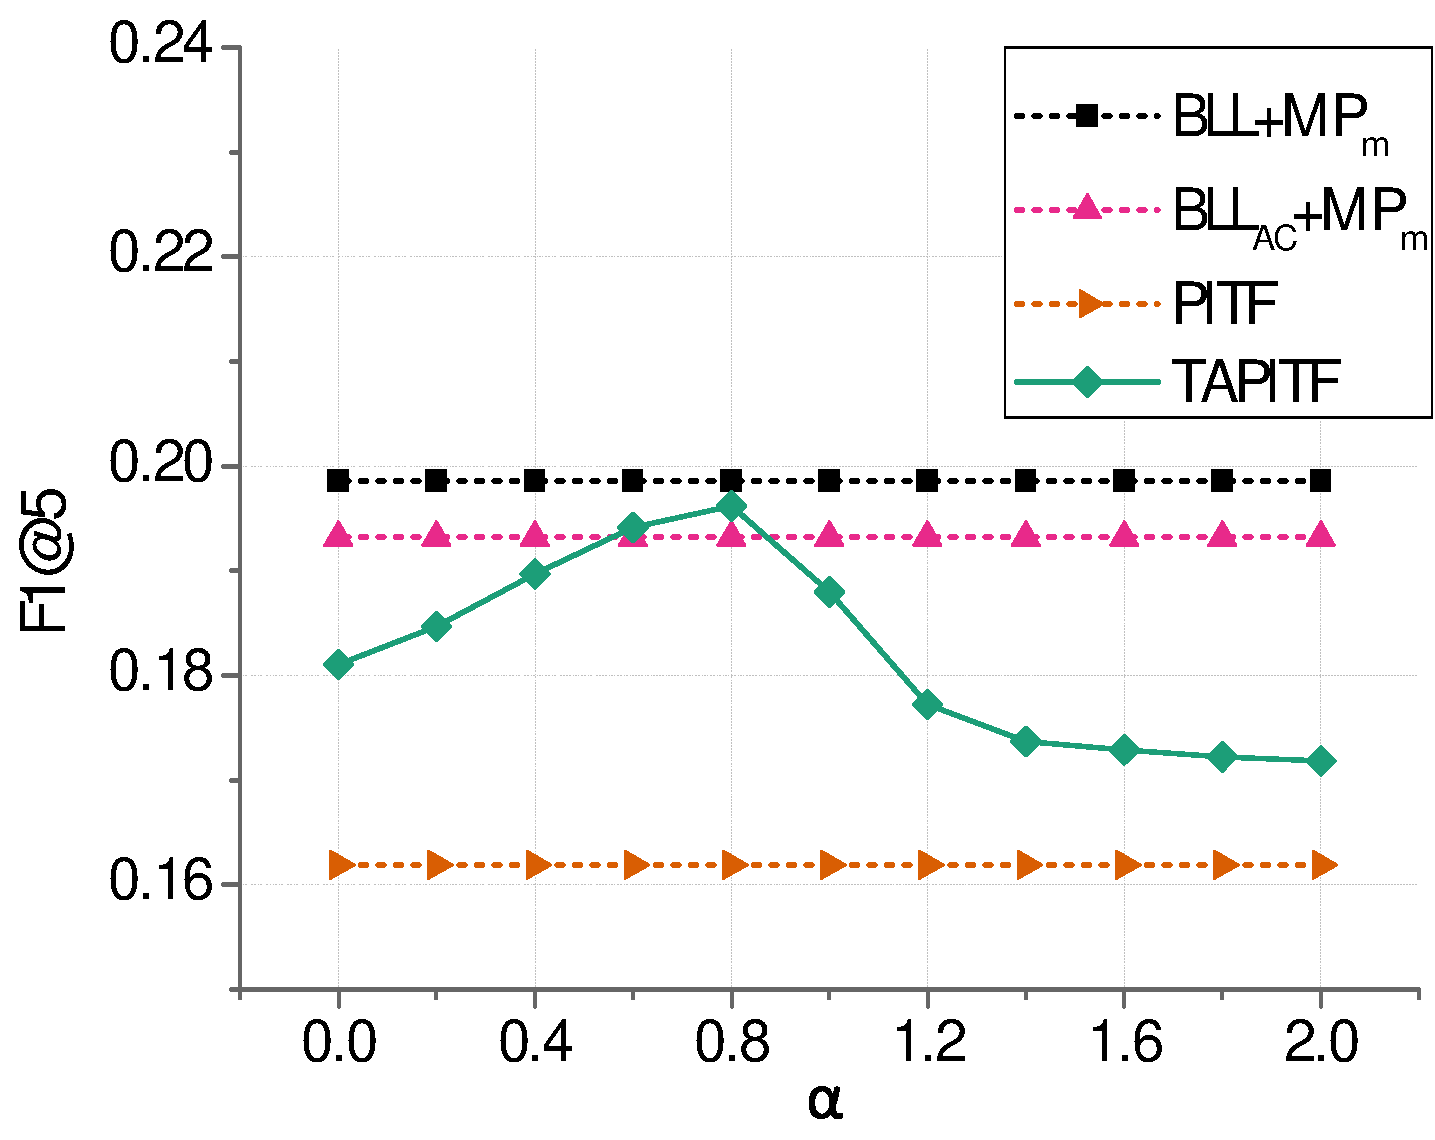
\includegraphics[width=0.485\textwidth]{Fig/wpitf/alphad1}}
	\hspace{0.0cm}
	\subfigure[Delicious (core 3)]{
		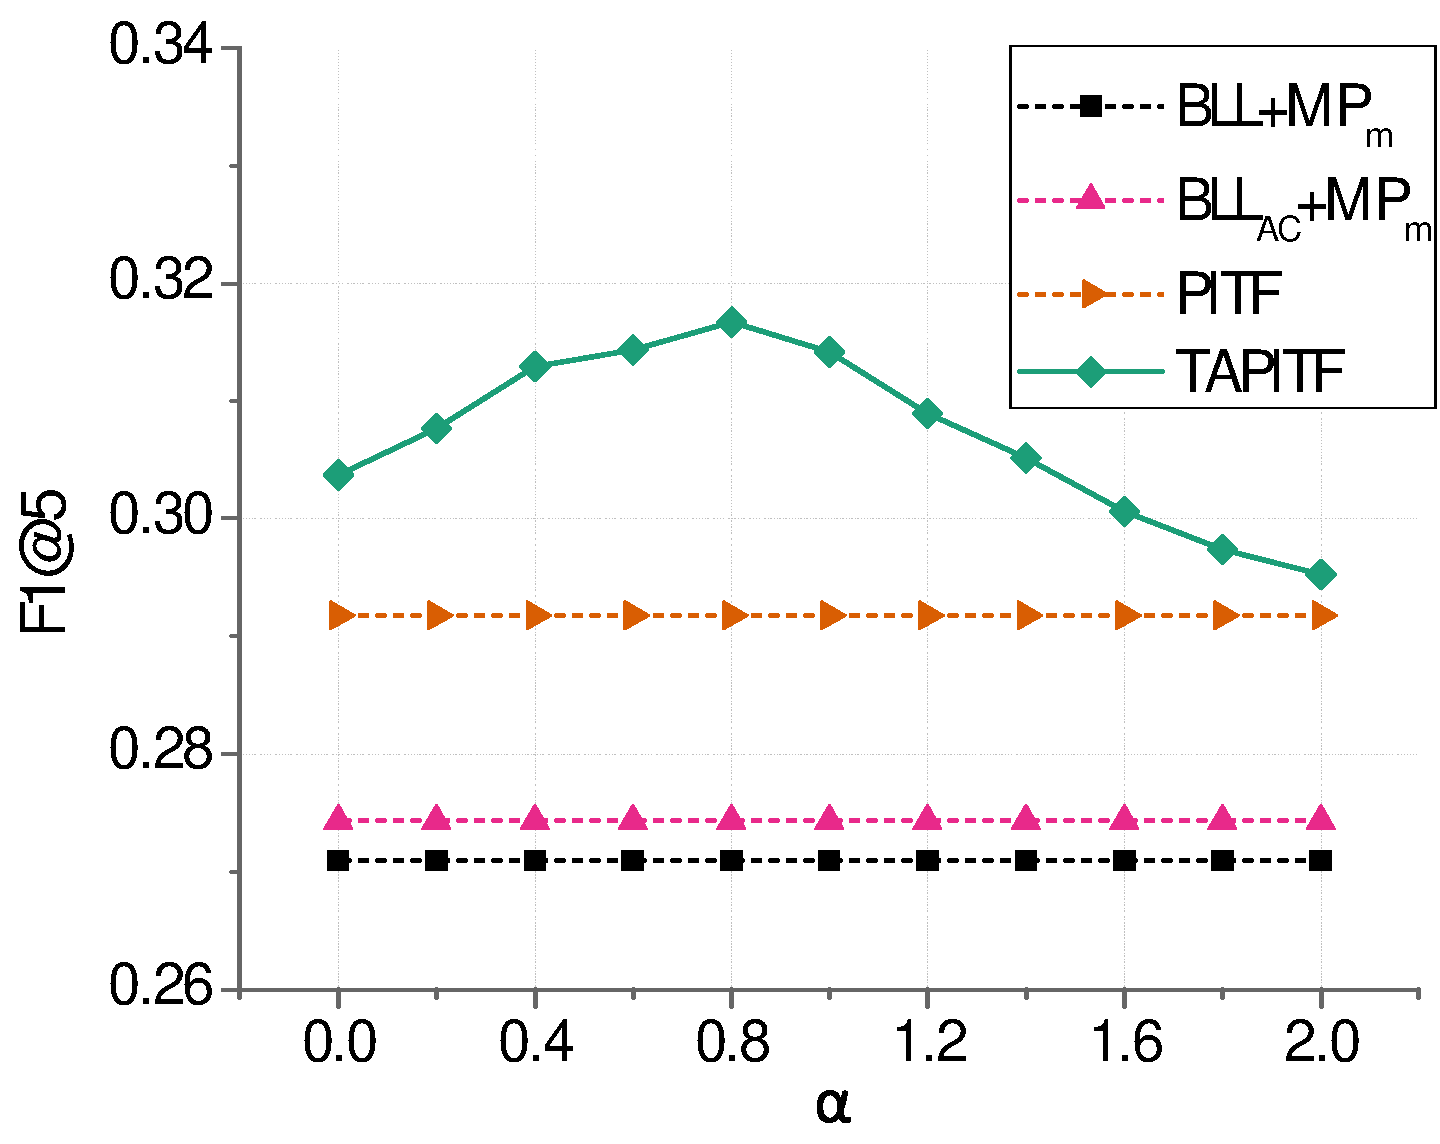
\includegraphics[width=0.485\textwidth]{Fig/wpitf/alphad3}}
    \caption{不同$\alpha$对推荐效果的影响}
	\label{fig-wpitf-alpha}
\end{figure}

\begin{figure}
	\centering
	\subfigure[Movielens (no core)]{
		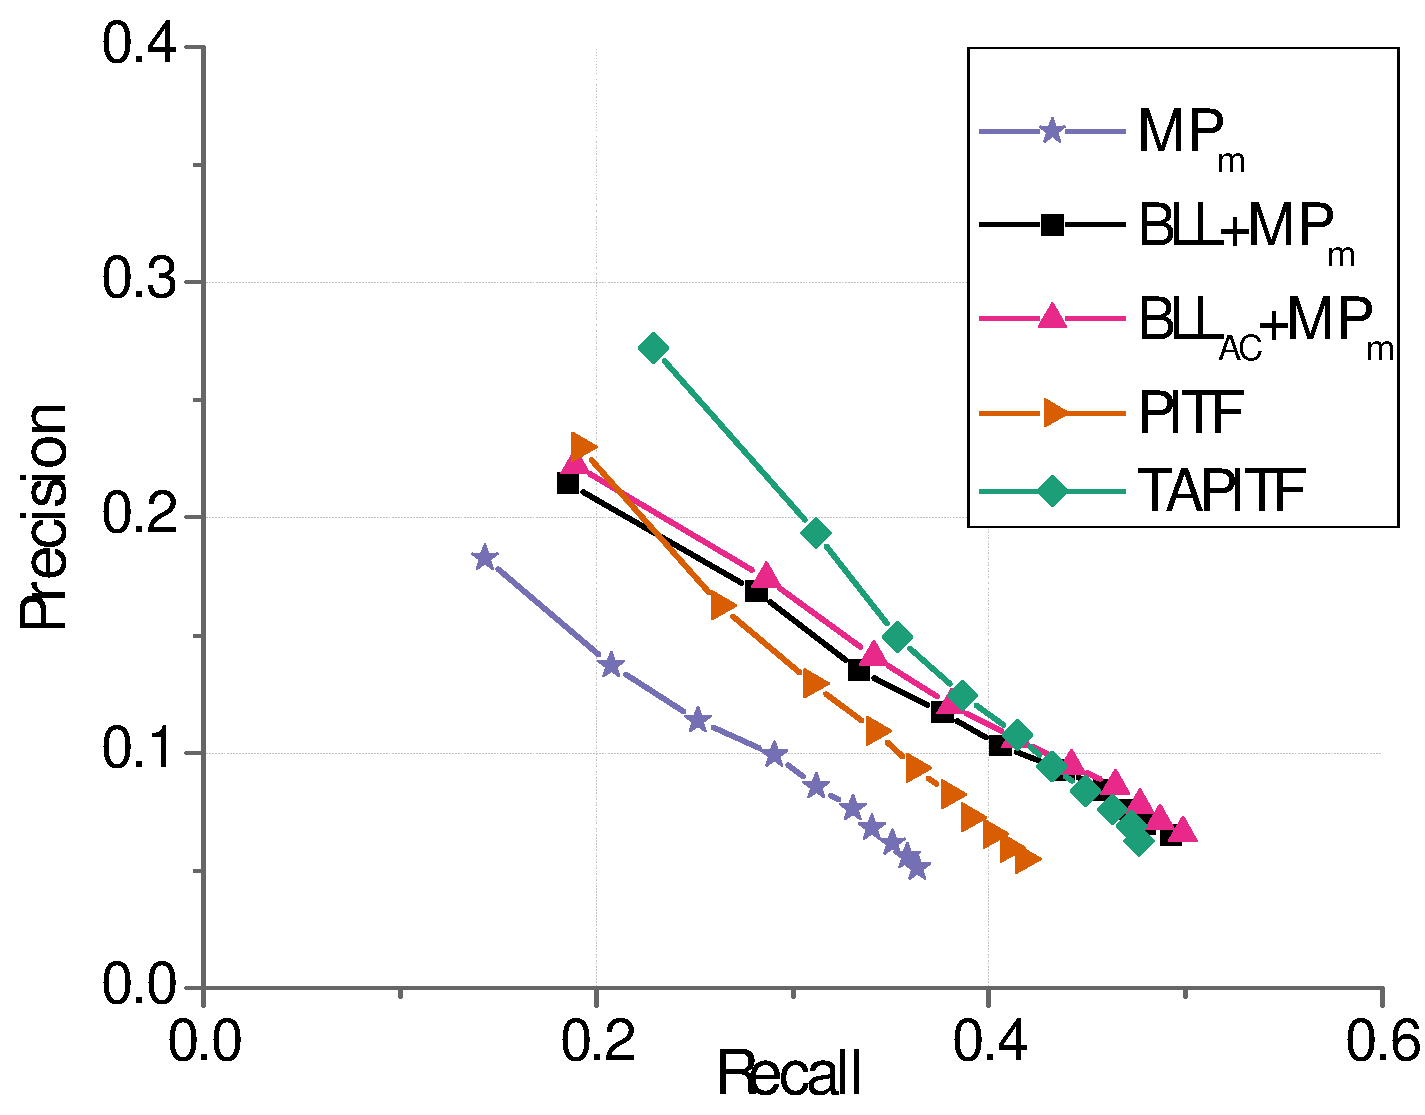
\includegraphics[width=0.485\textwidth]{Fig/wpitf/prm1}}
	\hspace{0.0cm}
	\subfigure[Movielens (core 3)]{
		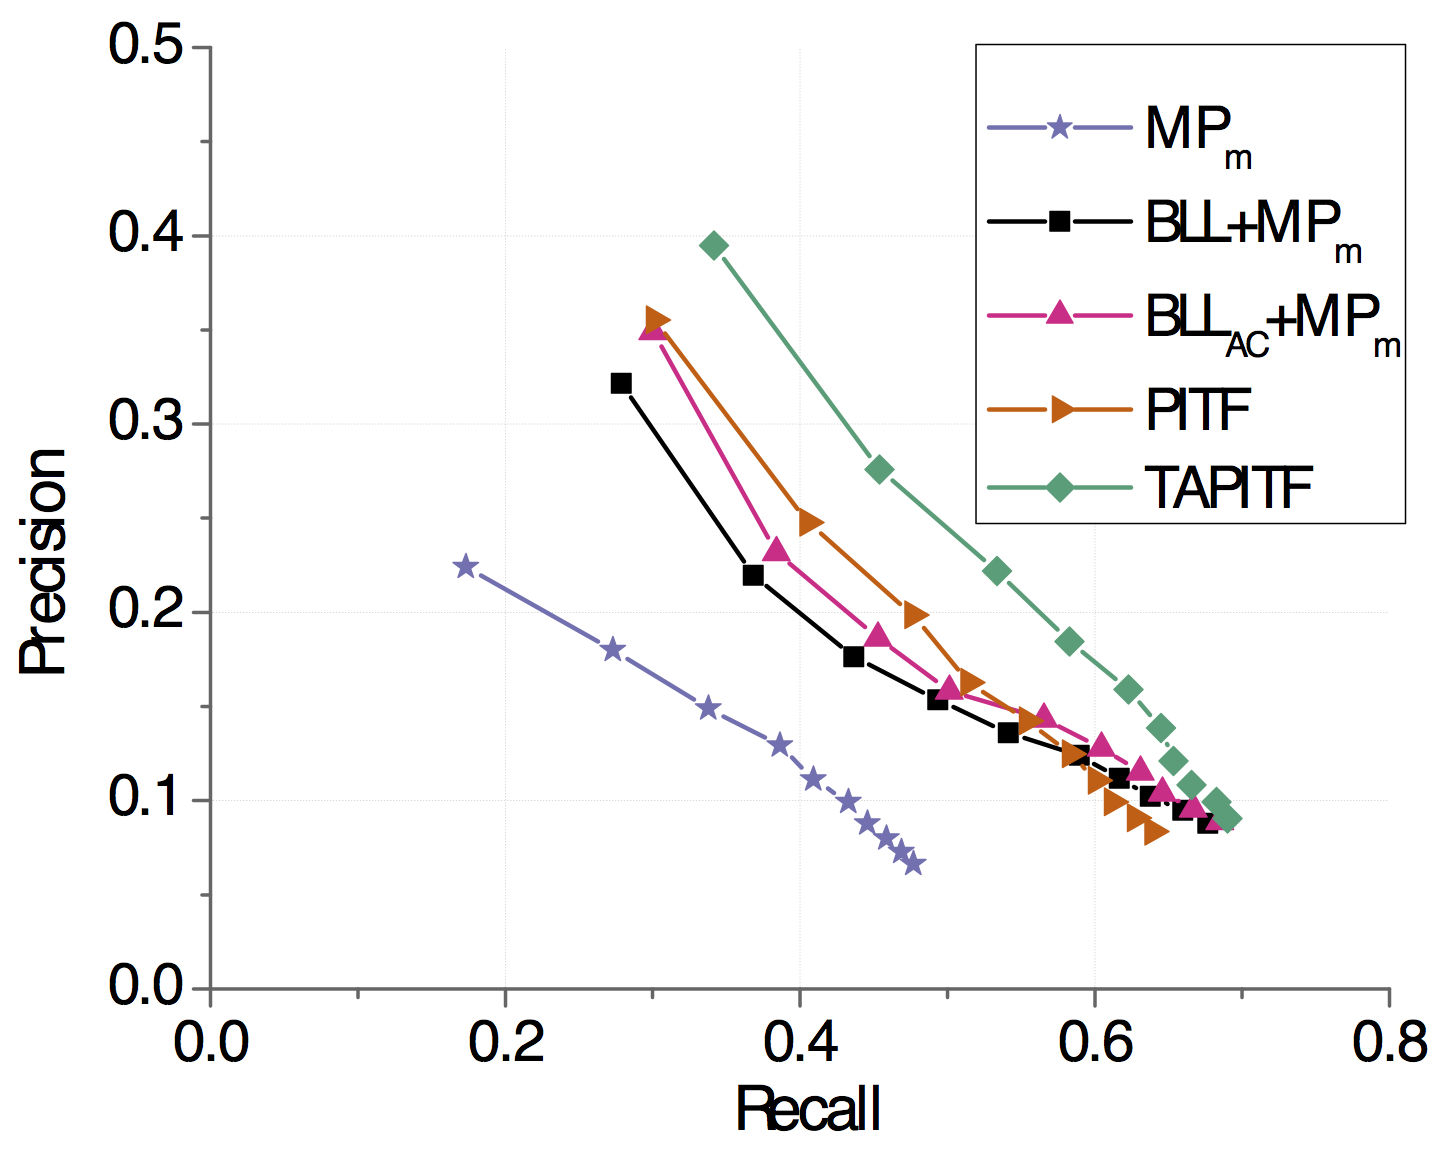
\includegraphics[width=0.485\textwidth]{Fig/wpitf/prm3}}
	\subfigure[LastFM (no core)]{
		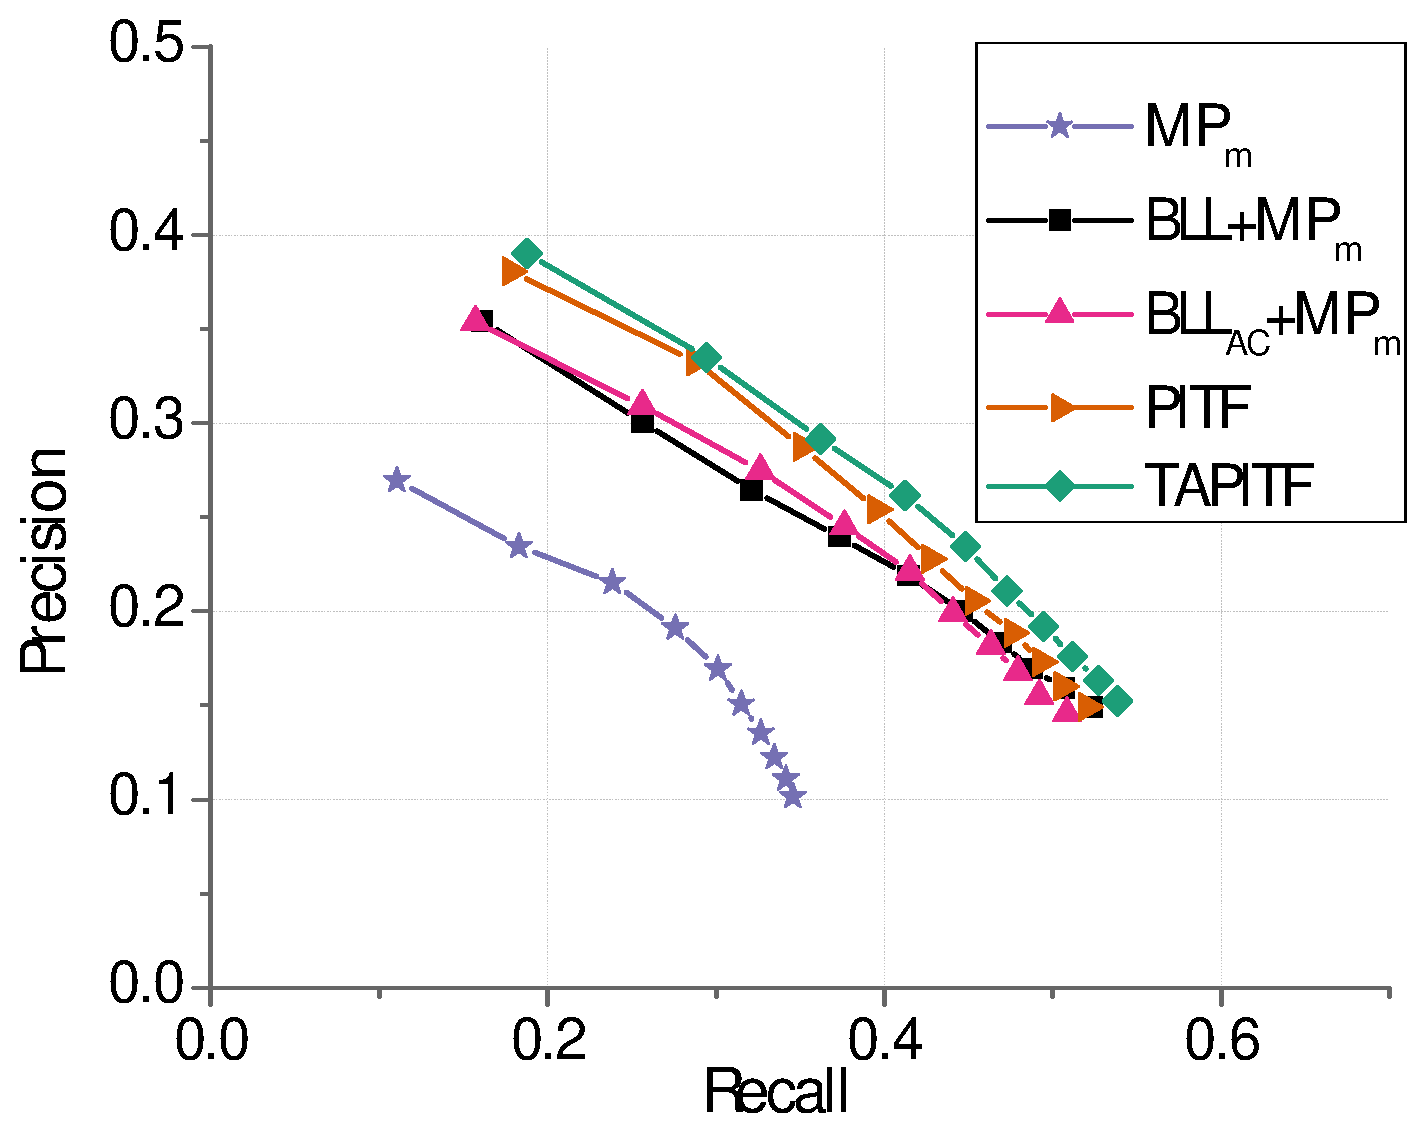
\includegraphics[width=0.485\textwidth]{Fig/wpitf/prl1}}
	\hspace{0.0cm}
	\subfigure[LastFM (core 3)]{
		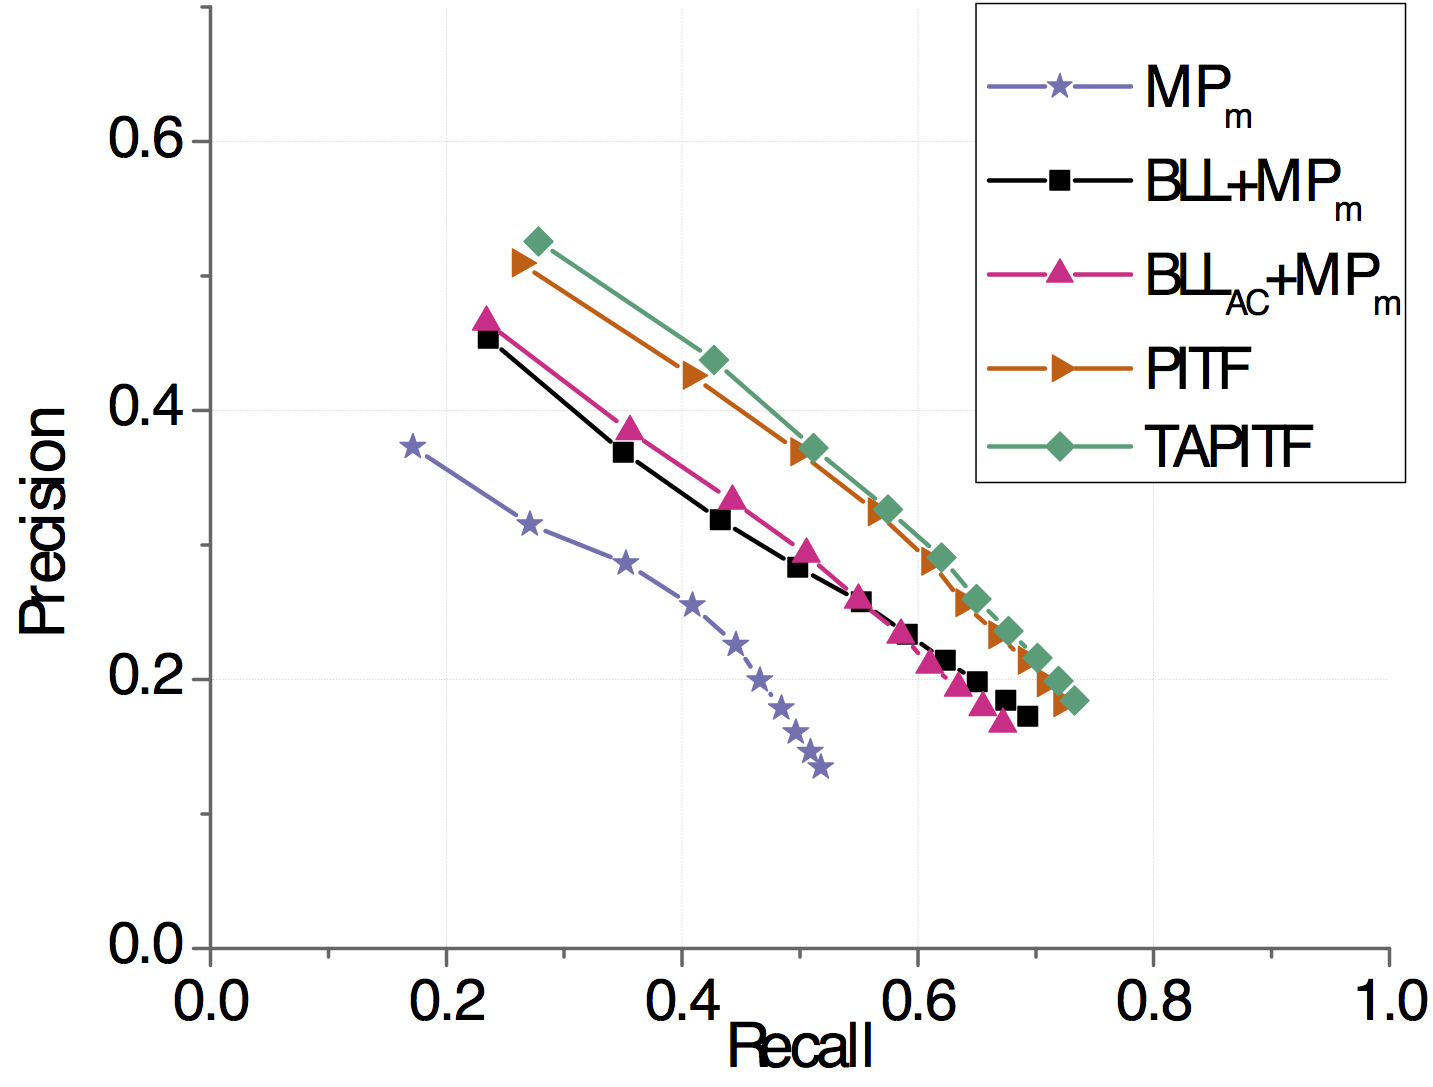
\includegraphics[width=0.485\textwidth]{Fig/wpitf/prl3}}
	\subfigure[Delicious (no core)]{
		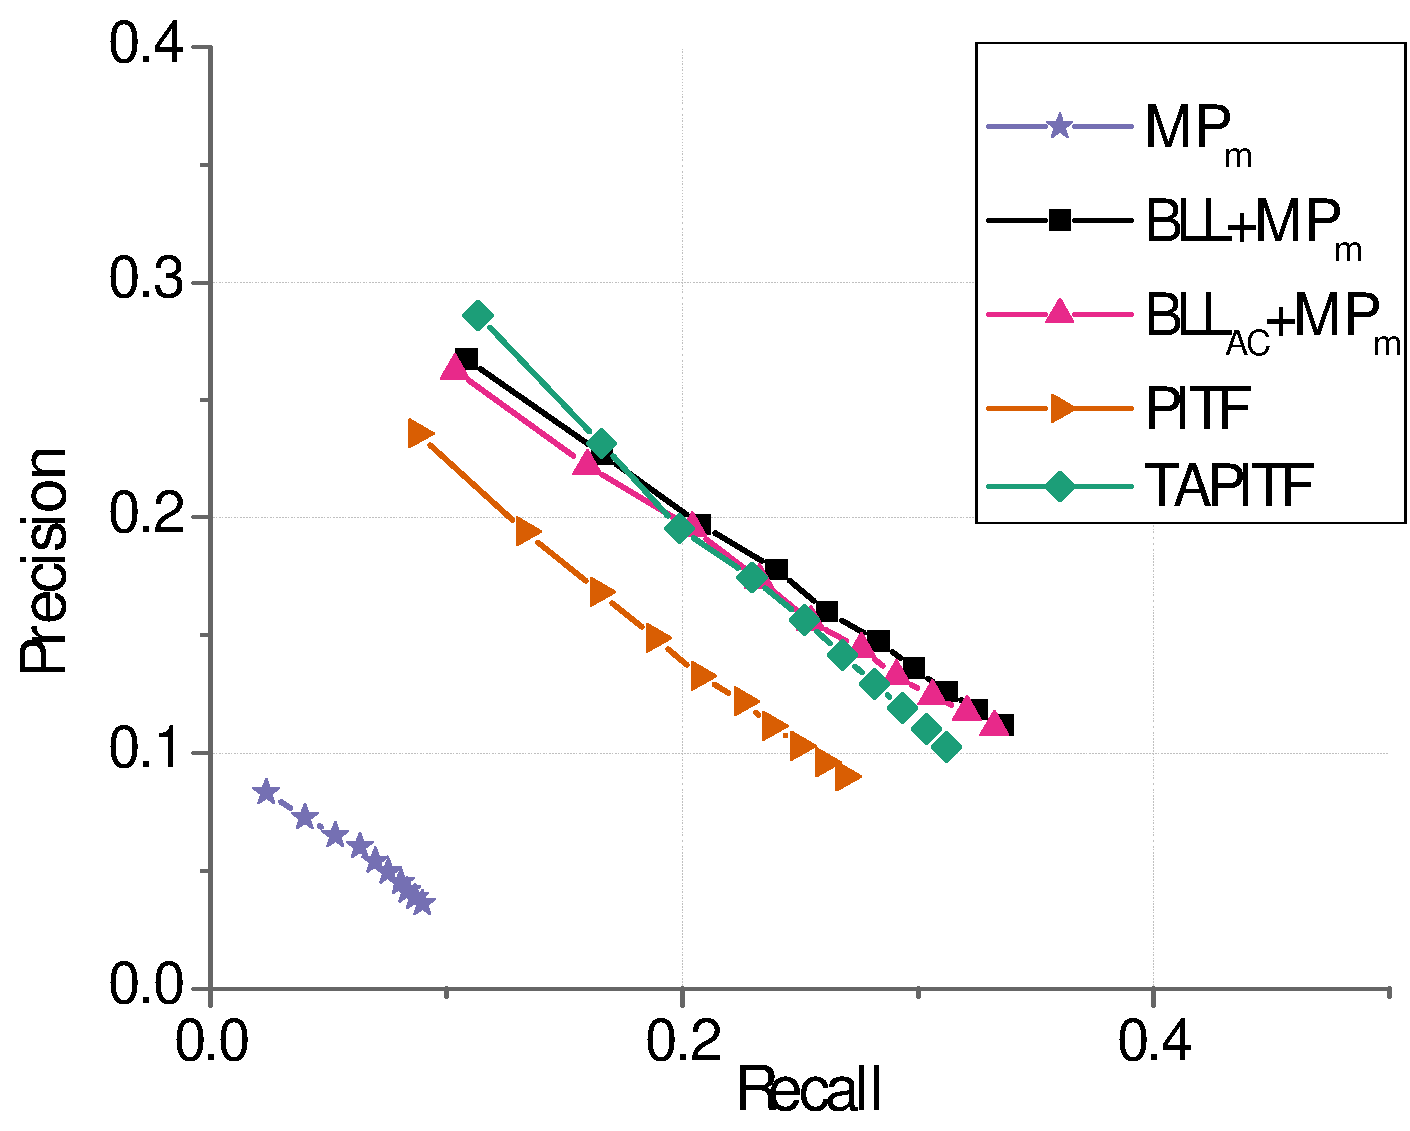
\includegraphics[width=0.485\textwidth]{Fig/wpitf/prd1}}
	\hspace{0.0cm}
	\subfigure[Delicious (core 3)]{
		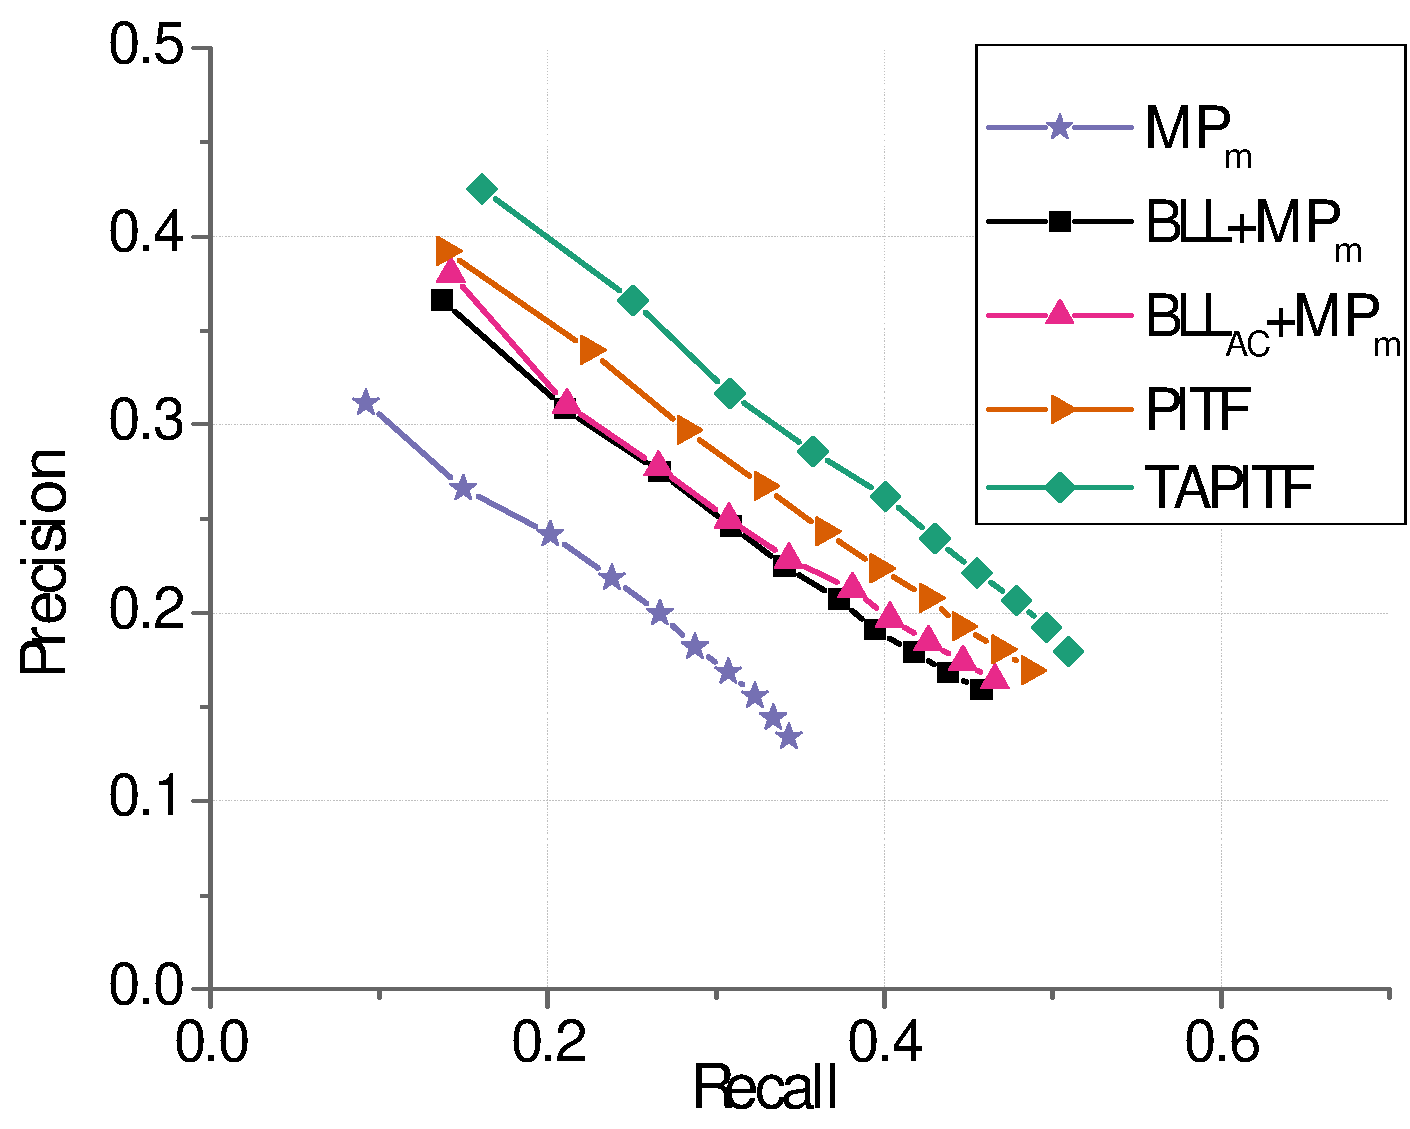
\includegraphics[width=0.485\textwidth]{Fig/wpitf/prd3}}
	\caption{各类标签推荐模型的召回率/精准率曲线}
	\label{fig-wpitf-pr}
\end{figure}

\subsubsection{权重因子 对 TAPITF 推荐结果的影响}
本小节中实验设置用户-标签-时间与商品-标签的权重因子相同,通过改变$\alpha$来观察 TAPITF 的性能 变化 (F1@5)。从图\ref{fig-wpitf-alpha}可以看出来,对所有的数据集, 随着$\alpha$值的增大,TAPITF 的性能不断提高,直到达 到最优值,继续增大$\alpha$,TAPITF 的性能会逐渐下降 (对数据集 LastFM core 3 的情况,如果将$\alpha$值调成负 数,那么 TAPITF 性能会明显下降,所以其最优值 就是在$\alpha=0$时取得)。当权重值$\alpha$调到最优时,可看
到TAPITF在所有数据集上基本都是优于 PITF 和 BLL+MP$_m$(最差也能与这两种方法持平),这说明通过 对 PITF 的用户-标签-时间与商品-标签上增加合理的 权重可以有效改善推荐性能。并且在对数据集过 滤之后 (core 3),可以看到 TAPITF 的性能明显优于其他对比方法。这有可能因为 PITF 对较稠密数据有 着更好的推荐效果,所以明显优于 BLL+MP$_m$,而本章提出的TAPITF方法在 PITF 的基础上考虑了时间对用 户行为的影响,性能得到进一步的提升。同时,实验结果中可以发现基于时间信息建模的标签推荐方法在冷启动方面要优于原始张量分解模型,体现这类方法在数据稀疏时的优势。

在接下来的实验中选择 TAPITF性能最好时的$\alpha$值来与其他模型的实验结果做对比,对数据集 Movielens core 3 取$\alpha=1.2$,对数据集 LastFM core 3 取$\alpha=0$,其他情况下均取$\alpha=0.8$。

\subsubsection{与其他标签推荐方法对比分析}

本小节实验将本章节提出的TAPITF模型与当前最新的一些标签推荐方法进行对比。图\ref{fig-wpitf-pr}显示在数据集 Movielens、LastFM 和 Delicious 上,TAPITF与其他标签推荐方法在TOP 1 到 TOP 10 上的召回率/精准率曲线。从总体上来说,对于所有数据集TAPITF基本上都是性能最优的,这进一步说明了在PITF中加 入时间对用户行为的影响是十分有效的。在未过滤的 数据集 Movielens 和 Delicous 上,尽管当推荐的 TOP n列表长度较大时,TAPITF性能略差于BLL+MP$_m$ 和 BLL$_{AC}$+MP$_m$,但是在实际应用中,对于一个给定的商品,用户关注的标签往往不会太多,有时甚至只会 关心排名最前的那个标签。所以在这种情况下,依然可以认为TAPITF方法是有效的。

在新颖性上,从表~\ref{tab-wpitf-aip}可以看出,PITF在所有数据集上的新颖性都是最好的,而TAPITF 的新颖性 略次于 PITF,但是优于 MP$_m$,BLL+MP$_m$ 和 BLL$_{AC}$+MP$_m$。 这说明TAPITF模型在获得最优准确度的前提下,还能得到较好的新颖度。而BLL类方法完全基于用户和商品的历史标签,导致新颖度非常低,这其实不利于推荐系统的发展。
\begin{table}
	\centering
	\caption{不同方法的AIP@10结果对比}
	\label{tab-wpitf-aip}%
	\begin{tabular}{|c||c|c|c|c|c|c|}
		\hline
		DataSet  & Core  & MP$_m$   & BLL+MP$_m$ & BLL$_{AC}$+MP$_m$ & PITF  & TAPITF \bigstrut \\
		\hline
		\hline
		\multirow{2}[4]{*}{Movielens } & -     & 0.806  & 0.788  & 0.786  & \textbf{0.854 } & 0.812  \bigstrut\\
		\cline{2-7}          & 3     & 0.761  & 0.762  & 0.757  & \textbf{0.803 } & 0.777  \bigstrut\\
		\hline
		\multirow{2}[4]{*}{LastFM } & -     & 0.732  & 0.724  & 0.709  & \textbf{0.779 } & 0.764 \bigstrut \\
		\cline{2-7}          & 3     & 0.668  & 0.660  & 0.639  & \textbf{0.697 } & \textbf{0.697 } \bigstrut\\
		\hline
		\multirow{2}[4]{*}{Delicious } & -     & 0.881  & 0.873  & 0.878  & \textbf{0.949 } & 0.912 \bigstrut \\
		\cline{2-7}          & 3     & 0.787  & 0.767  & 0.767  & \textbf{0.827 } & 0.778 \bigstrut \\
		\hline
	\end{tabular}%
	
\end{table}%
\subsubsection{TAPITF 对比 PITF}

图\ref{fig-wpitf-number}显示了 TAPITF 和 PITF 在不同迭代次数下
的准确度对比,为了确保算法达到收敛,本小节实验设置迭代轮数为100轮。从图中可以明显的看出,本章节提出的TAPITF 模型在数据集 Movielens、LastFM 以及 Delicious no core 和 core 3 上的准确度和收敛速度都要优于 PITF。TAPITF 在所有数据集上都能在40轮迭代前收敛,而PITF基本上要达到60轮迭代之后才逐渐收敛,而且 TAPITF在前20轮的收敛速度要远快于PITF,主要原因是加入了用户-标签-时间权重和商品-标签权重。因此即使不进行参数学习,TAPITF也可以拥有类似于BLL类模型的推荐效果。

而在运行时间上,相比 PITF,TAPITF由于在每轮迭代过程中要额外计算用户-标签-时间的权重因 子,所以每轮迭代的时间要比PITF慢。表 \ref{tab-wpitf-effiency}显示了 TAPITF与PITF在不同数据集上运行时间对比,本节实验选取了 100 轮迭代时间的平均值作为最终运行时 间(其中每轮迭代为训练集样本数目的 100 倍)。可以看出TAPITF在数据集 LastFM 和 Delicious 上的运行时间比PITF略长,而在数据集上Movielens上时间要比PITF长很多。但是如章节\ref{subsec-wpitf-timeAnalysis}所示,经过计算统计,因为在数据集 Movielens 上的期望值要比另外两个数据集大 10 倍以上,也就 是说 Movielens 的数据十分稠密,所以 TPWPITF 的 运行时间要比 PITF 长很多,而在当前互联网时代,数据往往都是非常稀疏的,所以在大多数情况下,本章模型仍然是十分有效的。

\begin{figure}
	\centering
	\subfigure[Movielens (no core)]{
		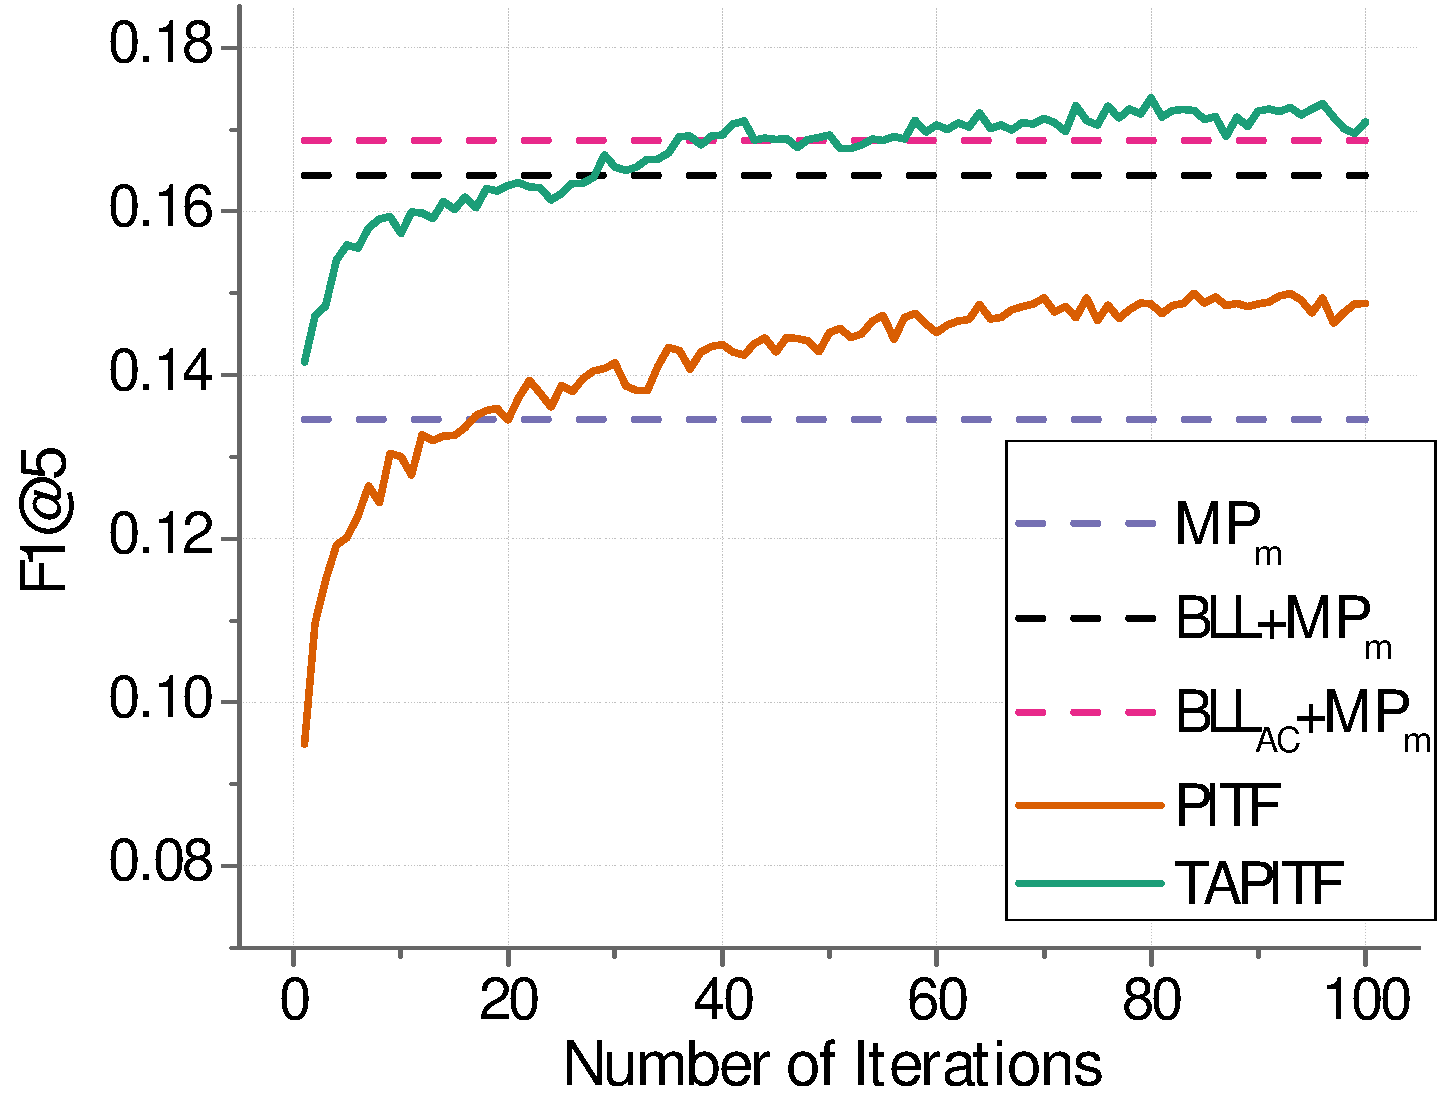
\includegraphics[width=0.45\textwidth]{Fig/wpitf/numberm1}}
	\hspace{0.8cm}
	\subfigure[Movielens (core 3)]{
		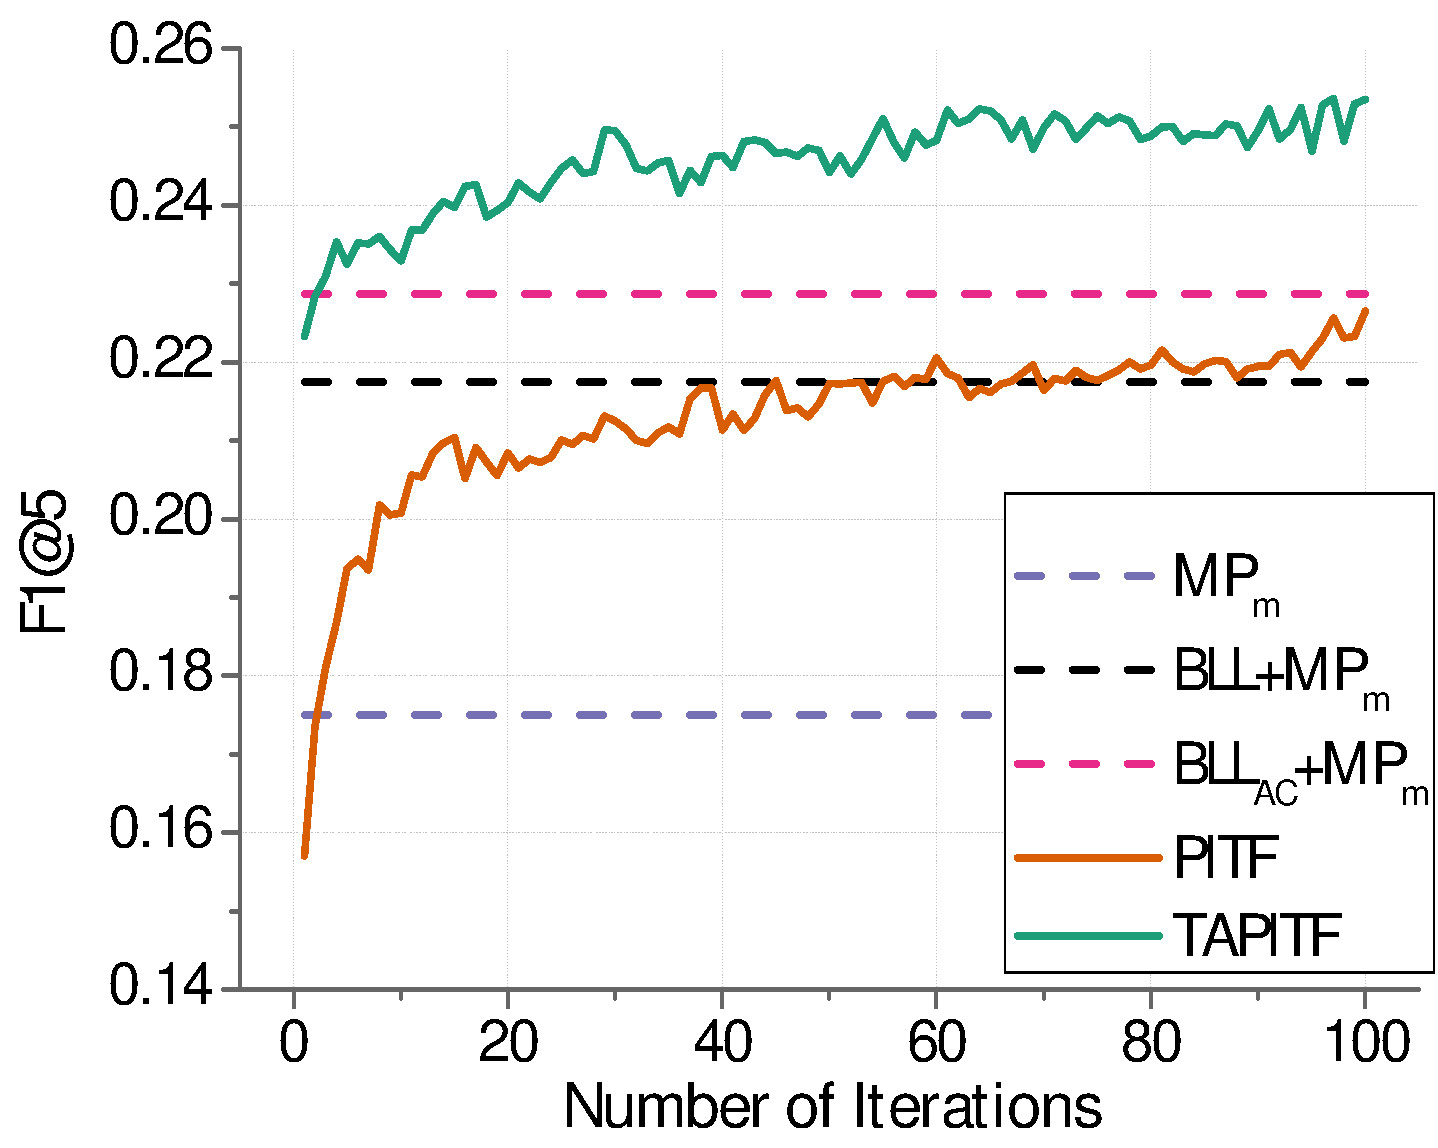
\includegraphics[width=0.45\textwidth]{Fig/wpitf/numberm3}}
	\subfigure[LastFM (no core)]{
		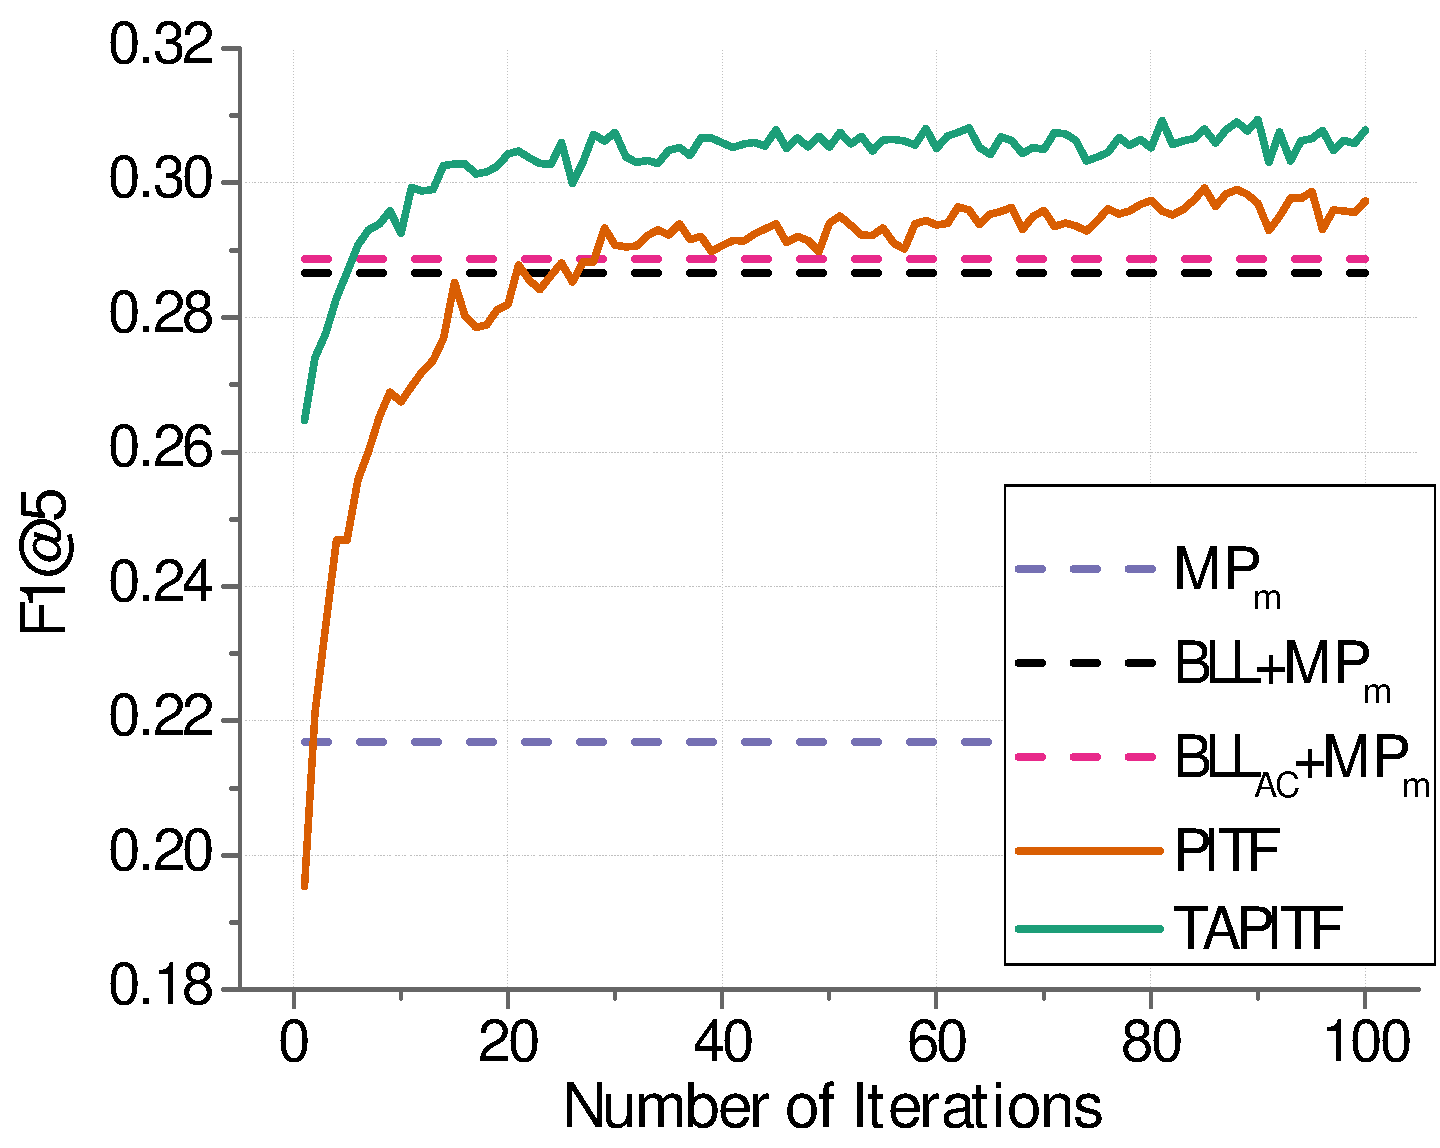
\includegraphics[width=0.45\textwidth]{Fig/wpitf/numberl1}}
	\hspace{0.8cm}
	\subfigure[LastFM (core 3)]{
		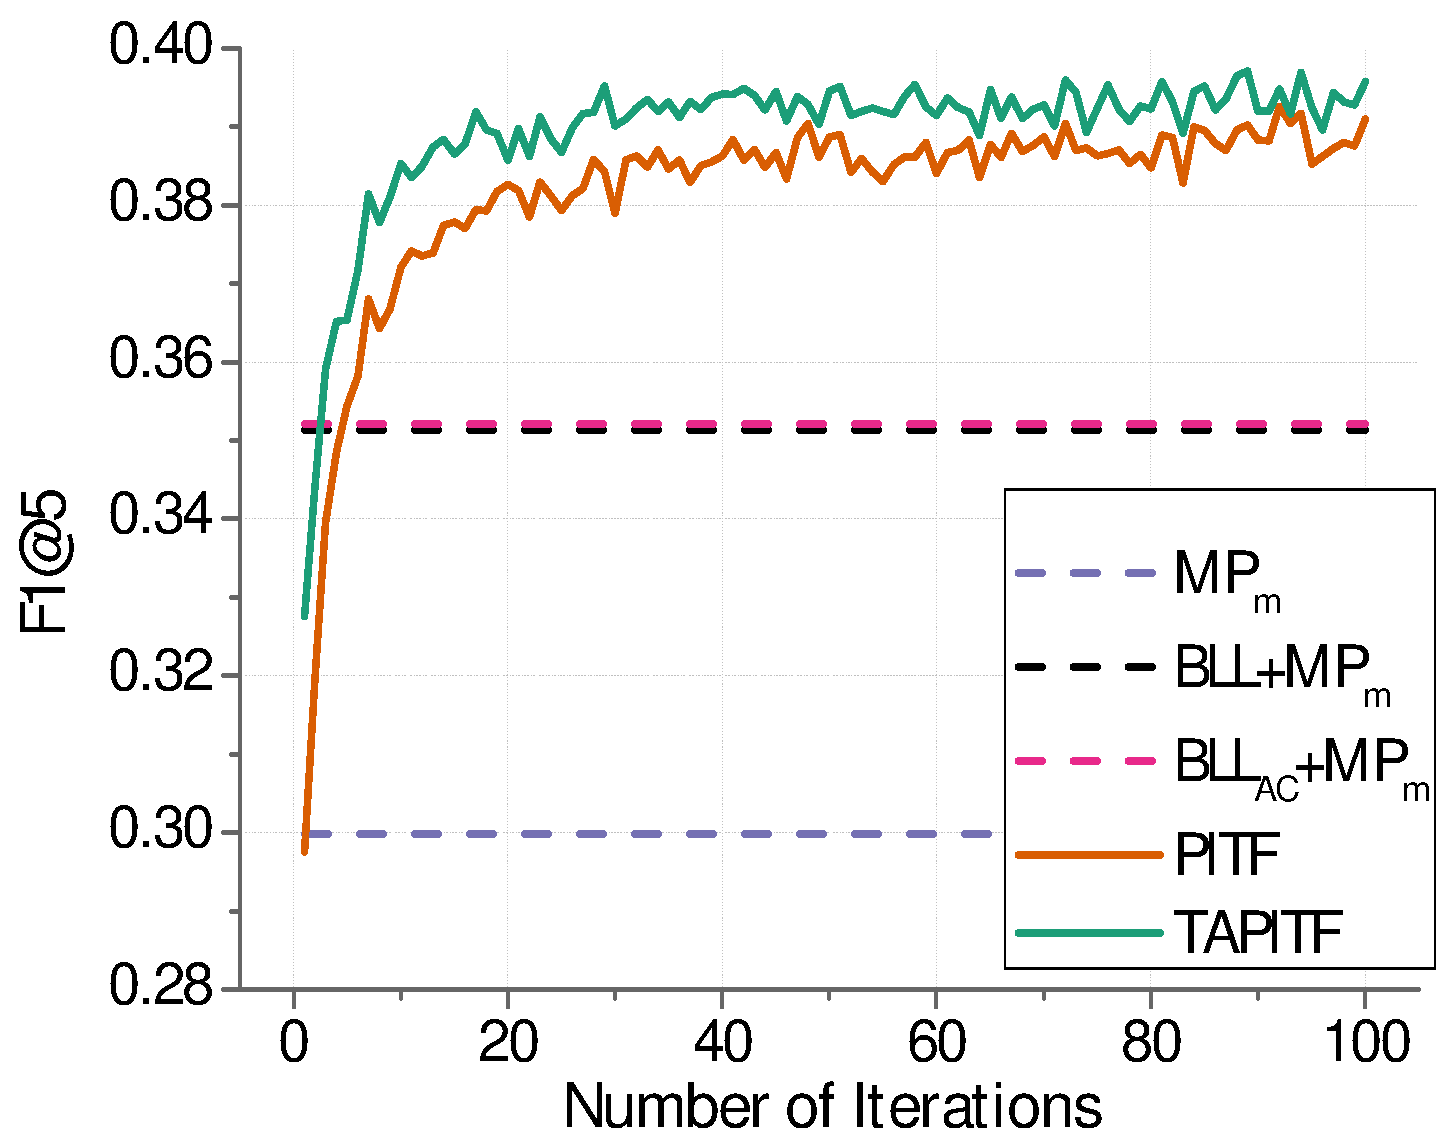
\includegraphics[width=0.45\textwidth]{Fig/wpitf/numberl3}}
	\subfigure[Delicious (no core)]{
		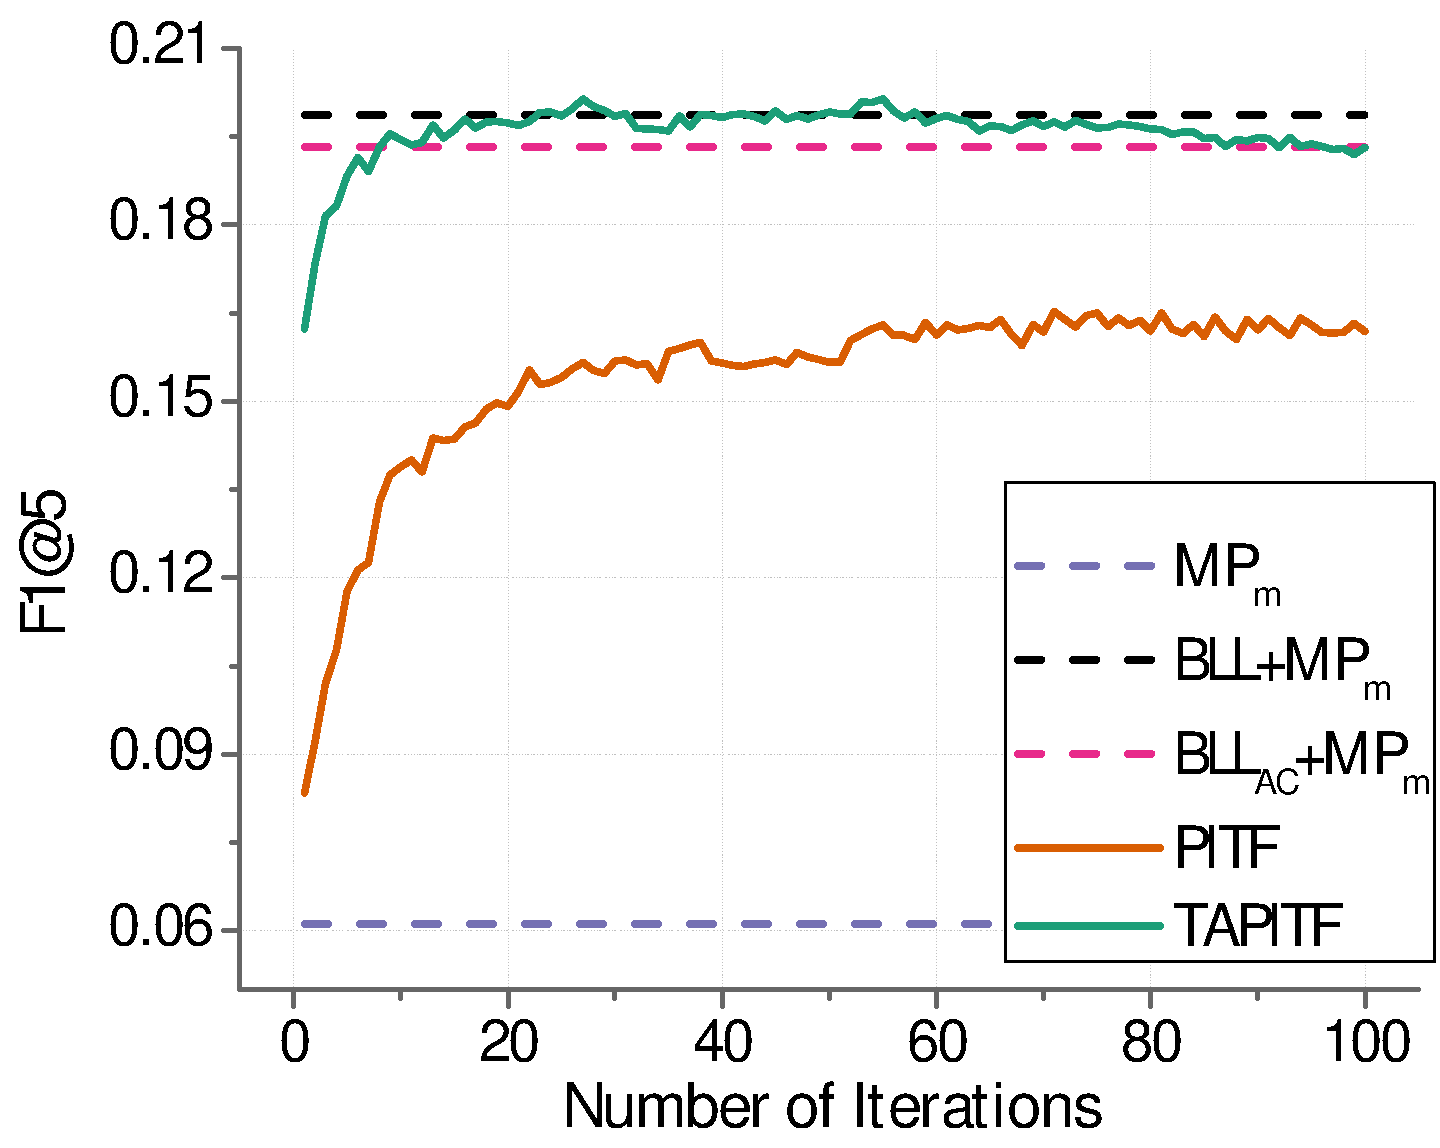
\includegraphics[width=0.45\textwidth]{Fig/wpitf/numberd1}}
	\hspace{0.8cm}
	\subfigure[Delicious (core 3)]{
		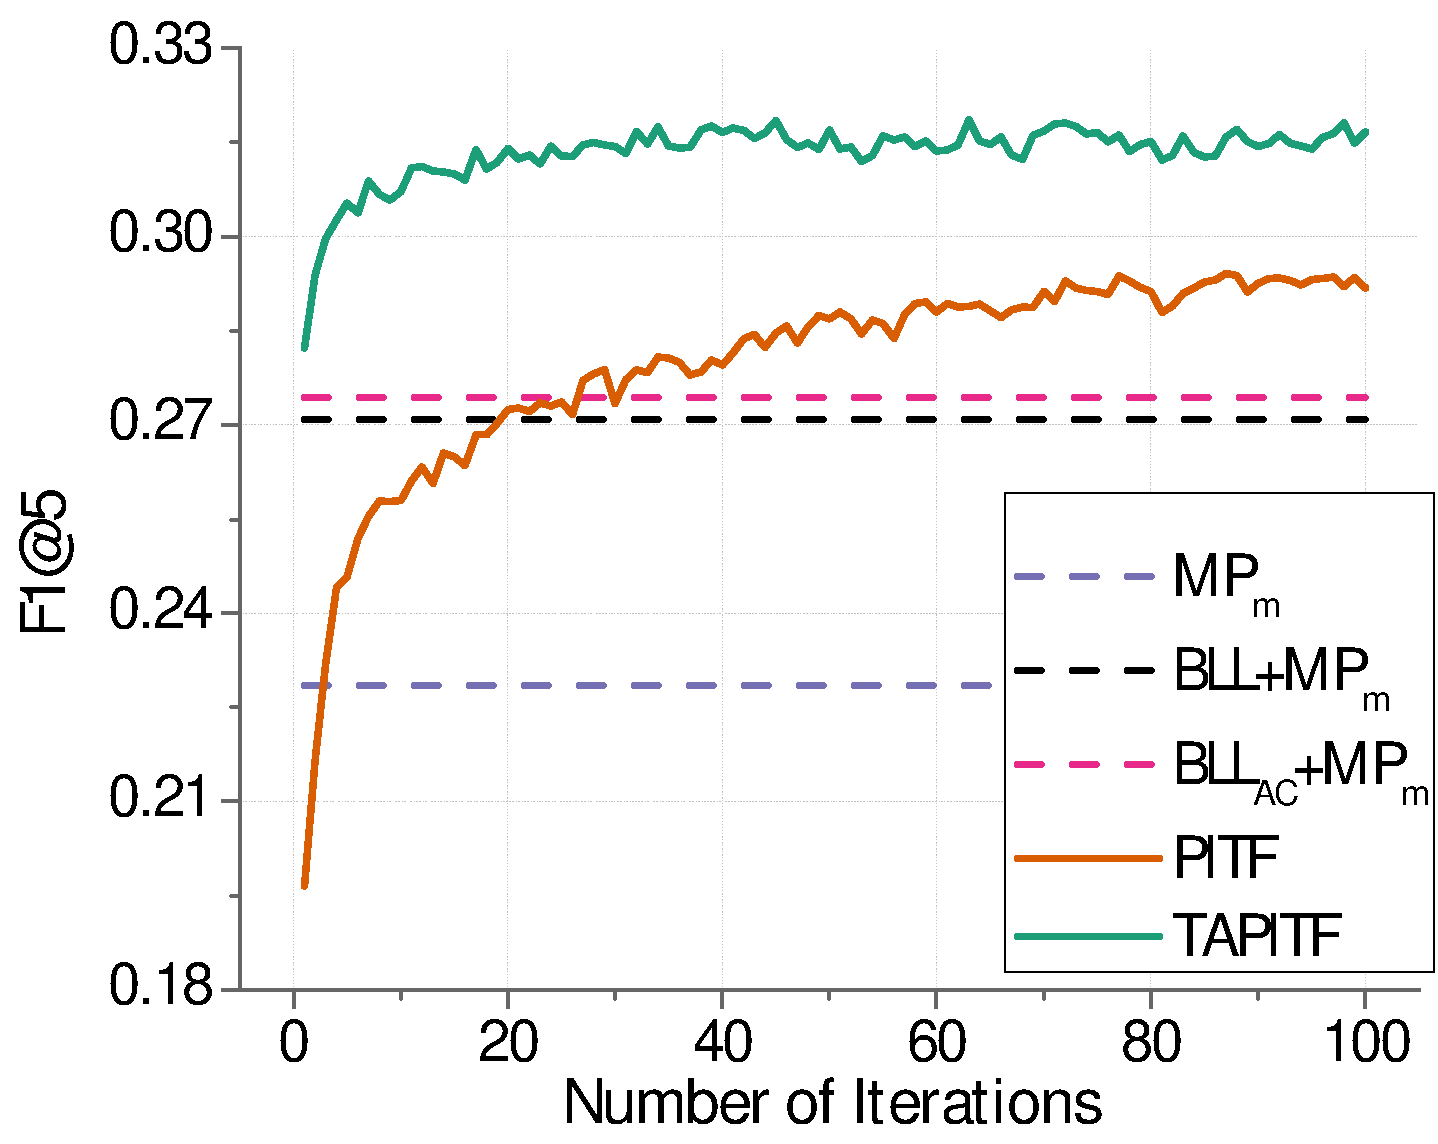
\includegraphics[width=0.45\textwidth]{Fig/wpitf/numberd3}}
	\caption{TAPITF 和 PITF的准确率与收敛速度对比}
	\label{fig-wpitf-number}
\end{figure}

\begin{table}
  \centering
  \caption{TAPITF 与 PITF的参数学习时间对比}
  	 \label{tab-wpitf-effiency}
    \begin{tabular}{|c||c|c|c|}
    \hline
    DataSet  & Core  & PITF  & TAPITF \bigstrut\\
    \hline
    \hline
    \multirow{2}[4]{*}{Movielens } & -     & 10.3  & 31.3  \bigstrut\\
\cline{2-4}          & 3     & 5.8   & 23.2  \bigstrut\\
    \hline
    \multirow{2}[4]{*}{LastFM } & -     & 41.4  & 51.7  \bigstrut\\
\cline{2-4}          & 3     & 32.6  & 44.6  \bigstrut\\
    \hline
    \multirow{2}[4]{*}{Delicious } & -     & 110.7  & 145.0  \bigstrut\\
\cline{2-4}          & 3     & 16.8  & 24.0  \bigstrut\\
    \hline
    \end{tabular}%

\end{table}%


\section{本章小结}
\label{sec-wpitf-conclusion}
本章节综合分析现阶段个性化标签推荐系统的优缺点,提出了时间感知的张量分解模型TAPITF。本章节工作从时间点过程对时间信息建模角度出发,利用指数函数将Hawkes过程从叠加转化为递归形式,使得计算用户当前时间对标签的喜好值只跟上次使用标签的时间有关,极大地减少了计算时间。然后,本章节工作将用户-标签-时间关系信息以及商品-标签关系信息以权重的方式与PITF模型结合,使得本章模型既能考虑用户标注标签行为随时间变化而变化的现象,也能有效地利用相似用户、相似商品、相似标签的信息,从而更好地对用户对商品标注标签的行为进行建模,提高标签推荐的准确度和新颖性。通过在不同场景的真实数据上进行实验,表明TAPITF在准 确性上优于当前流行的个性化标签推荐算法,同时有较好的推荐新颖性。

\clearpage
\phantom{s}
\clearpage
\chapter{总结与展望}

本文重点研究了基于矩阵分解相关理论的个性化推荐系统。本章对全文研究内容和技术模型进行总结归纳,并展望未来的重点研究工作。

\section{研究总结}


互联网发展以来,大量用户和企业产生了海量数据,面临着信息过载的问题。用户需要在大量无用信息中寻找少量自身感兴趣的信息,而企业也需要寻找与企业产品相关的目标用户,进行产品精准营销和推广。针对上述问题,个性化推荐系统应运而生,能够根据用户访问商品的历史行为数据建模,刻画用户和商品之间的交互关系,将可能感兴趣的商品推荐给目标用户。在使用互联网服务时,用户在网上寻找目标商品,遇到满意商品进行消费,然后进行显式评分,并利用标签描述商品的特点,且使用文本评价表达自己使用商品的感受。本文重点研究了上述的推荐场景,旨在解决三个相关问题:(1)\textit{商品推荐};(2)\textit{评分预测};(3)\textit{标签推荐}。\textit{商品推荐}主要是根据用户访问商品的历史行为,根据用户的个人喜好,推荐用户感兴趣的商品。\textit{评分预测}则是根据用户历史评分行为,预测用户对特定商品的满意程度。\textit{标签推荐}则是利用用户的历史使用标签的信息和特定商品的属性信息,个性化地推荐标签给用户来描述商品,方便用户输入。\textit{商品推荐}是推荐系统的主要目标,而好的\textit{评分预测}系统和\textit{标签推荐}系统则是有助于用户体验,并且促进推荐系统的良性循环。具体地,本文的研究问题和技术贡献总结如下。

首先,针对\textit{商品推荐},本文基于隐式反馈数据提出一种加权局部矩阵分解模型。传统加权矩阵分解模型基于全局低秩的假设,不能对隐式反馈数据的局部信息建模。而本文提出的模型设计了高效的子矩阵选择算法建模数据的局部信息,并改进了交替最小二乘算法进行子矩阵加权分解,刻画用户和商品的局部内在特征。并且,该模型带来两个额外好处,缓解了数据稀疏性问题和更好地进行分布式矩阵分解。基于公开的真实数据集的实验验证了该模型的有效性。

其次,针对\textit{评分预测},本文强调了局部矩阵分解模型在显式评分数据上的局部可解释性和目标一致性。近期的工作不能对数据的局部信息进行直观解释,并且分为两个步骤进行局部矩阵分解。基于此,本文结合主题模型和概率矩阵分解,提出多主题矩阵分解模型,该模型确保在同⼀个⽬标函数⾥分别对局部信息和用户、商品局部特征建模。此外,本文还利用狄利克雷分布和高斯-韦斯特分布作为模型参数的先验分布,得到全贝叶斯的多主题矩阵分解模型,使得模型对参数设置不敏感,并且能获得更加准确的评分预测。基于公开的真实数据集的实验验证了该模型在显式评分数据上进行评分预测的有效性,并能够对数据局部信息做出一定的解释。
	
最后,针对\textit{标签推荐},本文强调了标签的时间信息对标签推荐的帮助。现有的基于协同过滤模型的工作没有考虑用户使用标签的时间因素,并且协同过滤模型对新用户冷启动的标签推荐不友好。针对上述问题,本文提出了时间感知的张量分解模型,利用时间点过程对标签时间信息建模,并和逐对排序张量分解模型结合。基于公开数据集的实验表明该模型在准确性上优于当前流行的个性化标签推荐算法,同时具有可接受的推荐新颖性。

\section{研究展望}
本文重点研究了在用户的隐式反馈数据、显式评分数据和显式标签数据上的三个推荐系统相关问题。作者认为还可以从下面三个方面进行扩展。

首先,本文针对隐式反馈数据和显式评分数据进行了局部矩阵分解,需要对局部信息建模,增加了模型训练的时间和空间复杂度,尽管本文提出了一些改进的优化算法,但局部矩阵分解模型时间大于之前的单个全局模型。基于此,未来需要研究更高效的优化算法,加快模型参数学习效率。
	
其次,本文使用了较为规整的用户访问次数数据,评分数据以及标签数据。但推荐数据还包括许多其他数据,类似用户的评论文本数据,描述商品的图片数据以及领域数据(例如签到数据中地点位置信息,音乐中的音频数据等)。一些前人工作~\cite{he2015vbpr,li2016point,wang2017your,zheng2017joint}已经表明这类数据对提高个性化推荐系统的准确率都有极大的帮助。因此,如何融合多源数据也是未来研究的重点方向。
	
最后,本文提出的模型都是基于矩阵分解或者张量分解模型,都属于线性模型。但用户访问、评分、描述商品的行为是非常复杂的,受很多因素影响。因此,使用非线性模型,例如深度学习模型~\cite{wang2015collaborative,he2017neural},来捕捉这类复杂关系,能够更好地刻画用户画像和商品特性,也是未来研究的重点方向。

\clearpage
\phantom{s}
\clearpage



\clearpage

%额外空白页


\addcontentsline{toc}{chapter}{参考文献}
%\input D1-REFRENCE.tex

\begin{spacing}{1.2}
\bibliographystyle{gbt7714-2005}
\bibliography{bib/reference.bib}
\end{spacing}
%额外空白页
\clearpage
\phantom{s}
\clearpage

\pagestyle{plain}\clearpage
\pagestyle{plain}
\clearpage
\phantomsection
\addcontentsline{toc}{chapter}{附录}
\newpage
\chapter*{附录\quad 主要缩写符号对照表}
\vskip 5mm

\begin{tabular}{p{0.15\columnwidth}p{0.85\columnwidth}}
	ALS  & 交替最小二乘法(Alternating Least Square)  \\
	AUC  & ROC曲线下面积(Area under the ROC Curve)  \\
	BPMF  & 贝叶斯概率矩阵分解(Bayesian Probabilistic Matrix Factorization)  \\
	BPR  & 贝叶斯个性化排序(Bayesian Personalized Ranking)  \\
	ERR & 期望排序倒数(Expected Reciprocal Rank)  \\
	LDA  & 潜在狄利克雷分布(Latent Dirichlet Allocation)  \\
	MF  & 矩阵分解 (Matrix Factorization)  \\
	MRR  & 平均排序倒数 (Mean Reciprocal Rank) \\
	NDCG  & 归一化的贴现累计收益 (Normalized Discounted Cumulative Gain)  \\
	PLSA  & 概率潜语义分析 (Probabilistic Latent Semantic Analysis) \\
	PMF & 概率矩阵分解 (Probabilistic Matrix Factorization)  \\
	PITF & 成对相互张量分解(Pairwise Interaction Tensor Factorization)  \\
	RMSE & 均方根误差(Root Mean Square Error)\\
	ROC  & 受试者工作特征曲线 (Receiver Operating Characteristic Curve)  \\
	SGD & 随机梯度下降 (Stochastic Gradient Descent)  \\
	SVD & 奇异值分解 (Singular Value Decomposition)  \\
	TF  & 张量分解 (Tensor Factorization) \\
	WMF  & 加权矩阵分解(Weighted Matrix Factorization)  \\
\end{tabular}


%额外空白页
\clearpage
\phantom{s}
\clearpage
 

%\pagestyle{plain}
%\clearpage
%\phantomsection
%\addcontentsline{toc}{chapter}{致谢}
%{\kaishu
\chapter*{致\qquad 谢}
\begin{spacing}{1.5}

四年本科、五年硕博,回首这九年的华东师大求学时光,历经本科好友、硕士同门的陆续毕业,此刻我也将博士毕业,感慨良多。在此期间,有幸得到老师和亲友们的指导与帮助,在此谨对他们表示衷心的感谢!
	
首先,我要郑重地感谢我的本硕博导师王晓玲教授。每个人生命中都会遇到贵人,我想她就是我的贵人。
她为我们创造了良好的学习环境与氛围,在学习方法上的细心指导,在生活上的关怀支持。我依稀记得刚王老师在我刚读研时为我指明了研究的方向,读博迷茫期时对我的耐心开导和鼓励,以及即将毕业之际传授于我未来需要的宝贵的工作经验。在以后的人生道路上,我都会一直铭记她的教诲。

其次,我十分感谢复旦大学的沙朝锋副教授。沙老师深厚的数学功底和精彩地模型介绍,让我看到了数据挖掘技术的魅力。感谢华东师范大学金澈清教授在关于LBS相关研究中给予的大量帮助和指导,金老师对待问题的严谨性让我印象深刻。然后,我还要感谢中国人民大学的赵鑫老师。赵老师花费许多精力和时间与我讨论研究问题和研究方法,修改学术论文,让我学习了大量的学术论文写作技巧。也特别感谢华东师范大学周傲英副校长、钱卫宁教授、宫学庆教授、何晓丰研究员、张蓉教授、高明副教授和周敏奇副教授在日常学习中与研究生课程中给予的多方面帮助和指导。

另外,感谢所有读研期间陪伴我的同学和朋友,你们是我的美好记忆。感谢已经毕业的林煜明博士、王立博士、徐辰博士、王朝勇、胡颢继等师兄,以及马建松、江俊文、段小艺等师弟师妹,感谢你们在我研究生前期给予的学习上的帮助和生活上的快乐。感谢张凯、彭宏伟、靳远远,你们为我的论文提出了宝贵的修改意见。特别感谢陪我度过研究生时光的朱涛和张新洲,谢谢你们几年来对我的关心和包容。感谢一起毕业的纪文迪博士、房俊华博士、孔超博士、张俍博士和孟丹博士,与你们一起毕业是我的荣幸。也祝尙在奋斗的朱涛博士、庞艳霞博士、毛嘉莉博士、章志刚博士、周欢博士顺利完成学业,早日毕业。感谢在109实验室一起学习的梁磊、赵大鹏、刘志、宋光旋、李财政、夏得伦、张颖、吕晓强、刘小捷、屈稳稳、贺韵宇、周纯依、刘文焱等师弟师妹们。此外,我还想感谢本科室友邱星星、吴超凡、李博,以及硕士同学张磊、李勇峰、董绍婵和顾玲,谢谢你们当年的一起玩耍以及对我找工作时的帮助和关心。

最后,着重感谢我的父母,对我攻读博士学位的大力支持。感谢未婚妻的一直陪伴,你的理解和奉献使我能够无忧地学习,感谢这份许多年来历久弥坚的爱恋。

\end{spacing}
\vspace{0cm} \hspace{10.8cm}  王科强

\hspace{9.8cm}  二零一七年五月 }



\pagestyle{plain}
\clearpage 
\phantomsection


\addcontentsline{toc}{chapter}{发表论文和科研情况}
\newpage
\section*{\centering{\songti{攻读博士学位期间发表论文和科研情况}}}
%\vskip 5mm
{\heiti $\blacksquare$ 已公开发表论文}\vskip 5mm
\begin{spacing}{1}
\begin{enumerate}
	\item 第一作者,IJCAI 2016,CCF A 类会议,长文
	\item 第一作者,DASFAA 2016,CCF B 类会议,长文
	\item 第一作者,APWEB 2014,CCF C 类会议,长文
	\item 第一作者,DSEJ 2016,长文
	\item 第二作者,DASFAA 2014,CCF B 类会议,长文
	\item 第二作者,WAIM 2014,CCF C 类会议,长文
	\item 第二作者,SCC 2014,CCF C 类会议,长文
    \item 第二作者,NDBC 2014,demo
	\item 第二作者,FCS 2016,CCF C 类期刊,长文
	\item 第二作者,ICDE workshop 2016,CCF A 类会议workshop, EI,长文
	\item 第二作者,计算机学报2016,长文
	\item 第三作者,DASFAA workshop 2017,CCF B 类会议workshop,EI,长文
\end{enumerate}
\end{spacing}
%\bigskip\bigskip\bigskip
% \bigskip
% {\heiti $\blacksquare$ 尚未发表论文}\vskip 5mm
% \begin{spacing}{1.2}
% \begin{enumerate}
% 	\item \textbf{Keqiang Wang}, Yuanyuan jin, Hongwei Peng, Xiaoling Wang: Fast Weighted Tensor Factorization for Personality Dishes Recommendation. To be submitted to IJCAI 2017.

% \item \textbf{Keqiang Wang}, Yuanyuan jin, Hongwei Peng, Xiaoling Wang: Personality Tag Recommendation based on Local Time Perception. To be submitted to FCS 2017.
% \end{enumerate}
% \end{spacing}
%{\heiti $\blacksquare$ 攻读学位期间参加的科研项目}\vskip 5mm
%\vskip 3mm



\printindex
\end{document}